%# -*- coding: utf-8-unix -*-
%%==================================================
%% thesis.tex
%%==================================================

% 双面打印
\documentclass[master, fontset=adobe,openany, oneside]{sjtuthesis}
% \documentclass[bachelor, openany, oneside, submit]{sjtuthesis}
% \documentclass[master, review]{sjtuthesis}
% \documentclass[%
%   bachelor|master|doctor, % 必选项
%   fontset=fandol|windows|mac|ubuntu|adobe|founder, % 字体选项
%   oneside|twoside,        % 单面打印,双面打印(奇偶页交换页边距,默认)
%   openany|openright,      % 可以在奇数或者偶数页开新章|只在奇数页开新章(默认)
%   english,                % 启用英文模版
%   review,     % 盲审论文,隐去作者姓名、学号、导师姓名、致谢、发表论文和参与的项目
%   submit      % 定稿提交的论文,插入签名扫描版的原创性声明、授权声明 
% ]

% 逐个导入参考文献数据库
\addbibresource{bib/thesis.bib}
% \addbibresource{bib/chap2.bib}
\setlength{\itemsep}{20ex}
\begin{document}

% 无编号内容:中英文论文封面、授权页
%# -*- coding: utf-8-unix -*-
% !TEX program = xelatex
% !TEX root = ../thesis.tex
% !TEX encoding = UTF-8 Unicode
\title{基于微流控和机器视觉的秀丽隐杆线虫毒理芯片系统研究\footnote{本研究由上海市科委基础重大研发计划(17JC1401001)资助}}
\author{张维军}
\advisor{陈翔\quad{}副教授}
% \coadvisor{某某教授}
\defenddate{2019年1月7日}
\school{上海交通大学}
\institute{电子信息与电气工程学院}
\studentnumber{115039910077}
\major{集成电路工程专业}
\degreetype{工程硕士学位}

\englishtitle{Research on Chip System of C.elegans Toxicology Based on Microfluidic and Machine Vision}
\englishauthor{Weijun Zhang}
\englishadvisor{Prof. Xiang Chen}
\englishschool{Shanghai Jiao Tong University}
\englishinstitute{Dept. of Micro-Nano Electronics}
\englishmajor{Engineering of Integrated Circuits}
\englishdate{Jan, 2019}
\englishdegree{Master of Engineering}


%\maketitle

% \makeatletter
% \ifsjtu@submit\relax
  % 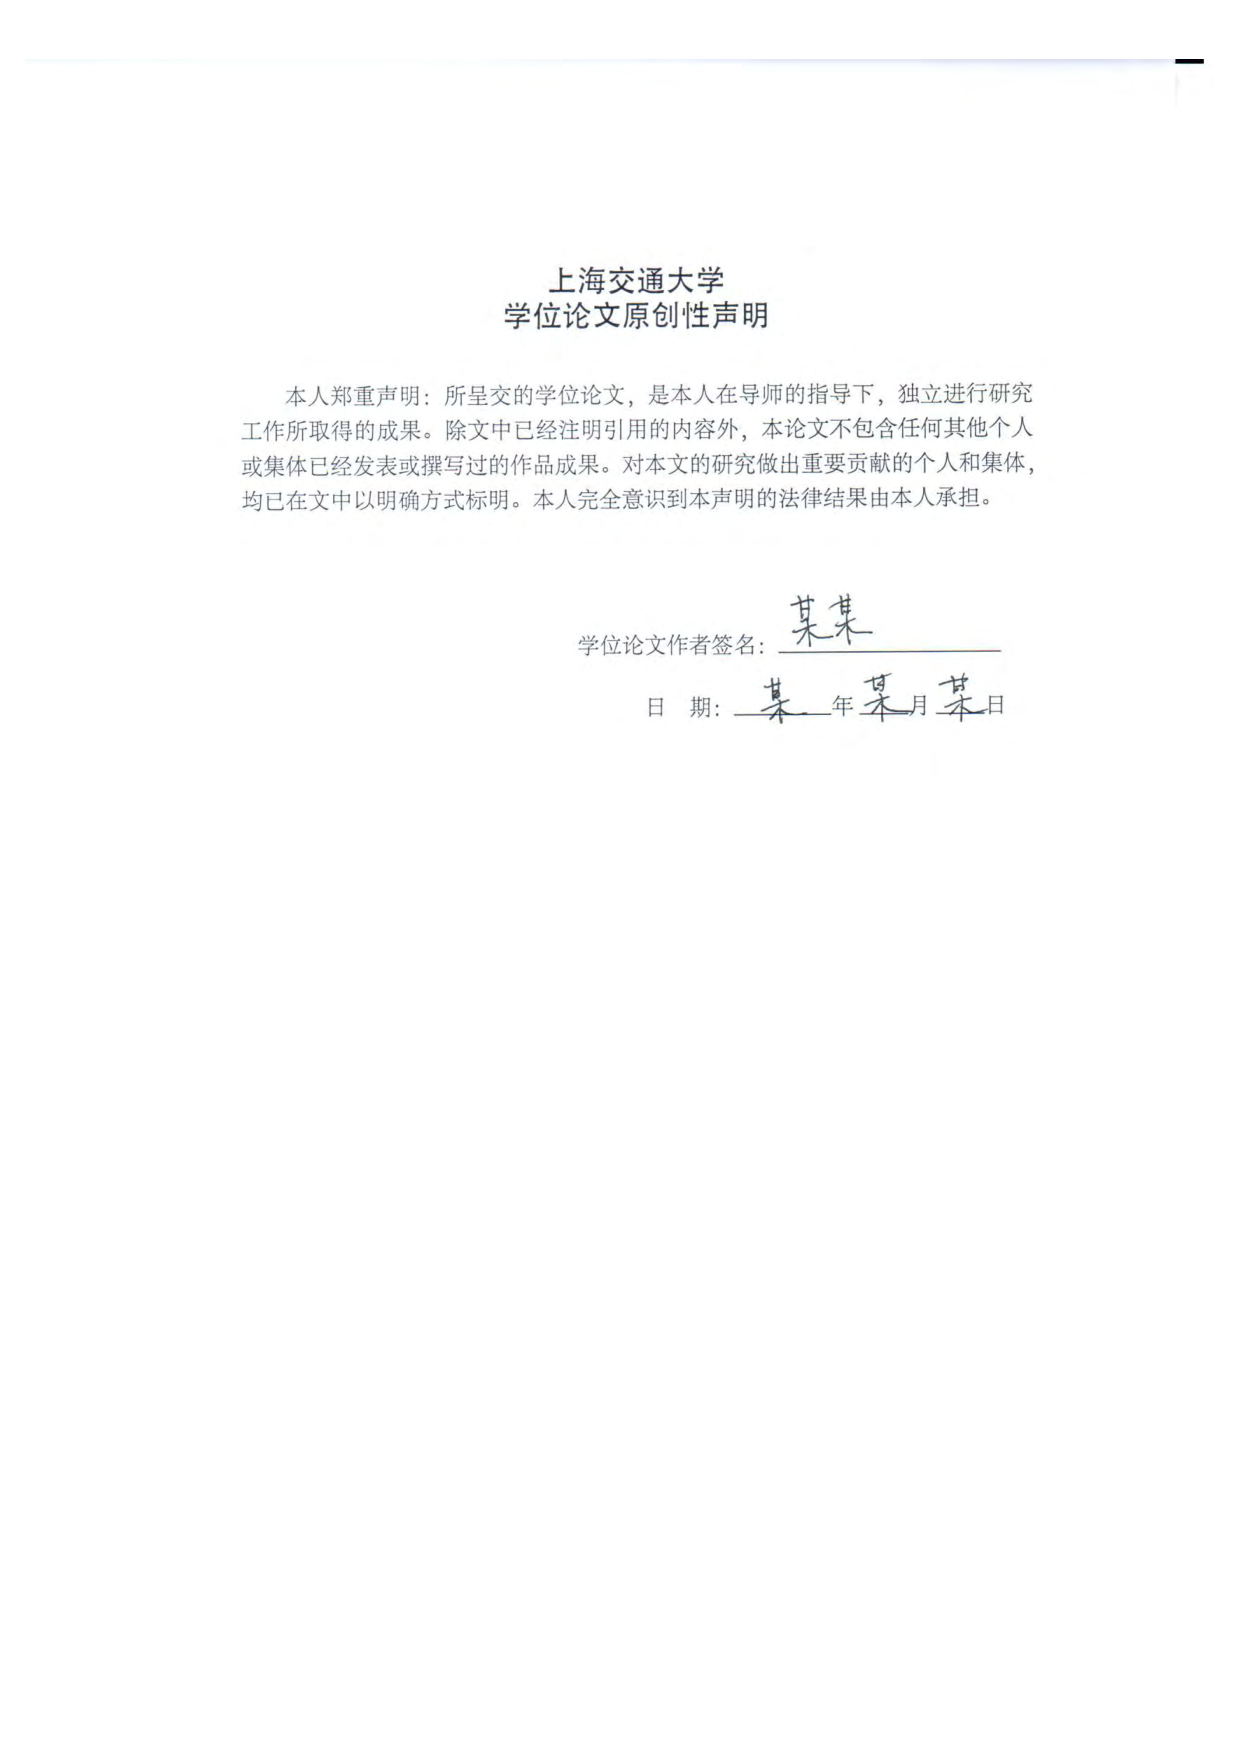
\includepdf{pdf/original.pdf}
  % \cleardoublepage
  % 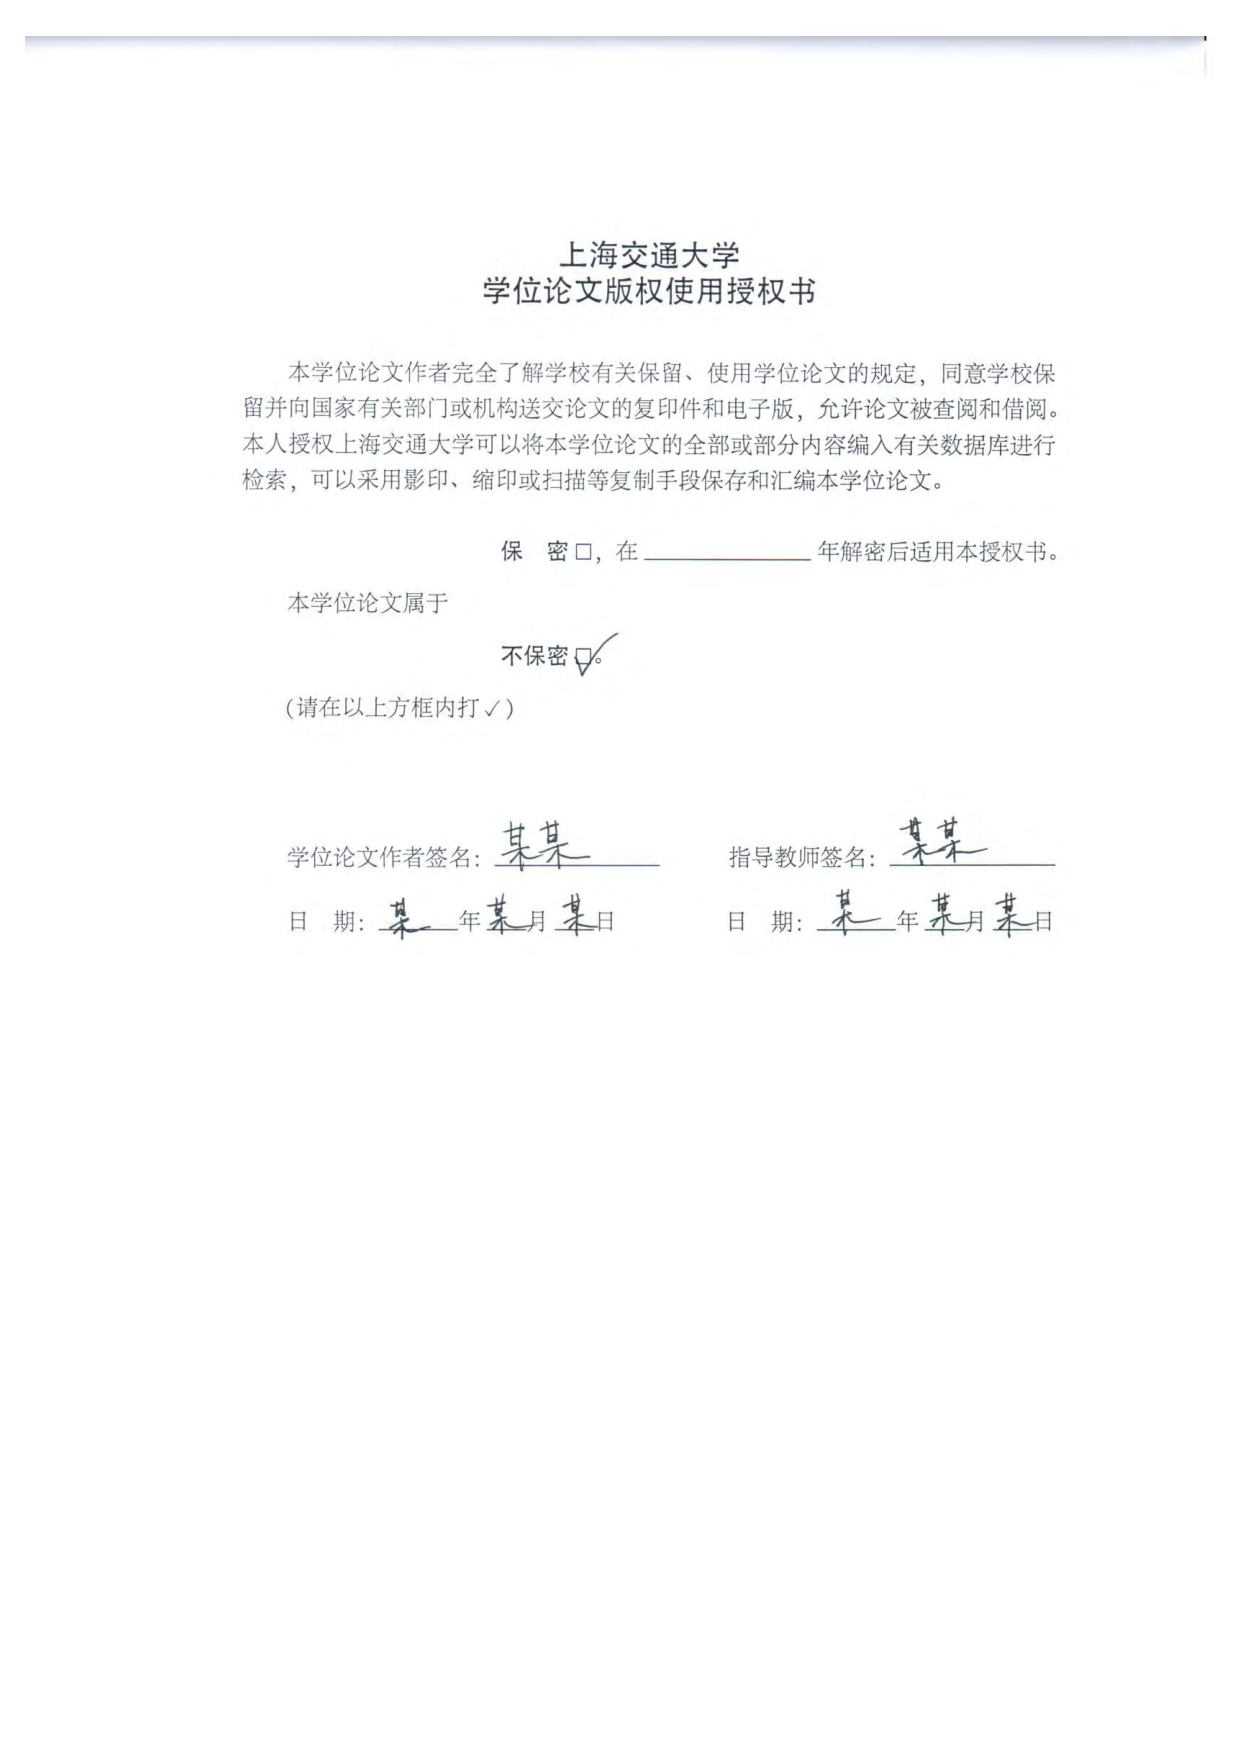
\includepdf{pdf/authorization.pdf}
  % \cleardoublepage
% \else
% \ifsjtu@review\relax
% % exclude the original claim and authorization
% \else
  % \makeDeclareOriginal
  % \makeDeclareAuthorization
% \fi
% \fi
% \makeatother

\frontmatter % 使用罗马数字对前言编号

% 摘要
%# -*- coding: utf-8-unix -*-
% !TEX program = xelatex
% !TEX root = ../thesis.tex
% !TEX encoding = UTF-8 Unicode
%%==================================================
%% abstract.tex for SJTU Master Thesis
%%==================================================

\begin{abstract}
	待完成
	
\keywords{\large 关键词一 \quad 关键词二 \quad 关键词三}
\end{abstract}

\begin{englishabstract}

	todo

\englishkeywords{\large keyword, keyword, keyword}
\end{englishabstract}



% 目录、插图目录、表格目录
\tableofcontents
% \listoffigures
% \addcontentsline{toc}{chapter}{\listfigurename}     % 将插图目录加入全文目录
% \listoftables
% \addcontentsline{toc}{chapter}{\listtablename}      % 将表格目录加入全文目录
% \listofalgorithms
% \addcontentsline{toc}{chapter}{\listalgorithmname}  % 将算法目录加入全文目录

%%# -*- coding: utf-8-unix -*-
% !TEX program = xelatex
% !TEX root = ../thesis.tex
% !TEX encoding = UTF-8 Unicode
\begin{nomenclaturename}
\label{chap:symb}

\begin{longtable}{rl}
$\epsilon$     & 介电常数 \\
 $\mu$ 		& 磁导率 \\
 $\epsilon$     & 介电常数 \\
 $\mu$ 		& 磁导率 \\
 $\epsilon$     & 介电常数 \\
 $\mu$ 		& 磁导率 \\
 $\epsilon$ 	& 介电常数 \\
 $\mu$ 		& 磁导率 \\
 $\epsilon$     & 介电常数 \\
 $\mu$ 		& 磁导率 \\
 $\epsilon$     & 介电常数 \\
 $\mu$ 		& 磁导率 \\
 $\epsilon$     & 介电常数 \\
 $\mu$ 		& 磁导率 \\
 $\epsilon$ 	& 介电常数 \\
 $\mu$ 		& 磁导率 \\
 $\epsilon$     & 介电常数 \\
 $\mu$ 		& 磁导率 \\
 $\epsilon$     & 介电常数 \\
 $\mu$ 		& 磁导率 \\
 $\epsilon$     & 介电常数 \\
 $\mu$ 		& 磁导率 \\
 $\epsilon$ 	& 介电常数 \\
 $\mu$ 		& 磁导率 \\
 $\epsilon$     & 介电常数 \\
 $\mu$ 		& 磁导率 \\
 $\epsilon$     & 介电常数 \\
 $\mu$ 		& 磁导率 \\
 $\epsilon$     & 介电常数 \\
 $\mu$ 		& 磁导率 \\
 $\epsilon$ 	& 介电常数 \\
 $\mu$ 		& 磁导率 \\
 $\epsilon$     & 介电常数 \\
 $\mu$ 		& 磁导率 \\
 $\epsilon$     & 介电常数 \\
 $\mu$ 		& 磁导率 \\
 $\epsilon$     & 介电常数 \\
 $\mu$ 		& 磁导率 \\
 $\epsilon$ 	& 介电常数 \\
 $\mu$ 		& 磁导率 \\
 $\epsilon$     & 介电常数 \\
 $\mu$ 		& 磁导率 \\
 $\epsilon$     & 介电常数 \\
 $\mu$ 		& 磁导率 \\
 $\epsilon$     & 介电常数 \\
 $\mu$ 		& 磁导率 \\
 $\epsilon$ 	& 介电常数 \\
 $\mu$ 		& 磁导率 \\
 $\epsilon$     & 介电常数 \\
 $\mu$ 		& 磁导率 \\
 $\epsilon$     & 介电常数 \\
 $\mu$ 		& 磁导率 \\
 $\epsilon$     & 介电常数 \\
 $\mu$ 		& 磁导率 \\
\end{longtable}

\end{nomenclaturename}
 % 主要符号、缩略词对照表

\mainmatter % 使用阿拉伯数字对正文编号

% 正文内容
%# -*- coding: utf-8-unix -*-
%%==================================================
%% chapter01.tex for SJTU Master Thesis
%%==================================================

\chapter{绪论}
\label{chap:intro}

\section{论文研究的背景及意义}
\label{sec:intro:analog}
	20 世纪以来,人类生存环境中化学品日益增多,对数量巨大且种类复杂的
	化学物进行健康风险的评估是公共健康领域当前重要的研究课题。此外,人类与
	环境化合物的接触方式多为低剂量下的复合暴露,如何实现高通量的毒性评价和
	科学的风险评估成为研究的热点与难点。
	
		自 2005 年起,美国启动了 21 世纪毒理学研究计划(TOX21),主要借助体
	外测试和计算生物信息学等方法进行高通量化学品毒性评估。然而,使用细胞或
	类器官的体外方法虽然可以进行较高通量的毒性测试,但无法代替动物体内实
	验,因为其结果无法反映化合物进入生物体内吸收、分布、代谢与排泄环节对毒
	性的影响。传统的动物体内毒性研究结果具有很大的参考意义,但是实验周期长、
	成本高,并且涉及动物保护与伦理。如果进行待测化合物低剂量复合暴露毒性研
	究,需要不同化合物的多剂量进行配伍,基于上述动物实验的局限性,难以进行
	高通量的毒性测试。秀丽隐杆线虫作为一种模式生物,对环境变化非常敏感;其
	生命周期和寿命较短,身体尺寸较小易操作,以大肠杆菌为食易培养,身体透明
	易观察,染色体和基因组较小易分析,生物学信号通路保守,因此近年来线虫被
	广泛应用于重金属、PM2.5、农药、纳米颗粒和有机污染物等环境毒理学研究领
	域。国际上目前已进展到第三阶段的 TOX21 计划也在使用包括线虫在内的模式生
	物对前期结果进行验证,并计划对更多环境化合物进行毒性筛选。
	
		传统的线虫培养方法在液体或琼脂板上进行,需要的线虫数量多,待测化合
	物所需量较大,此外难以对单个线虫实现精确刺激、操控和追踪。微流控体系与
	线虫大小尺度相匹配,有望实现线虫芯片内培养、成像和数据分析等。自从 2011
	年美国启动“类器官芯片”计划之后,以微流控芯片为平台的毒理测试技术发展
	迅速,相比器官芯片平台,线虫芯片是在动物个体水平上进行毒理学研究,具有
	不可替代的优势。
	
\section{秀丽隐杆线虫概述}
	\begin{figure}[h]
	  \centering
	  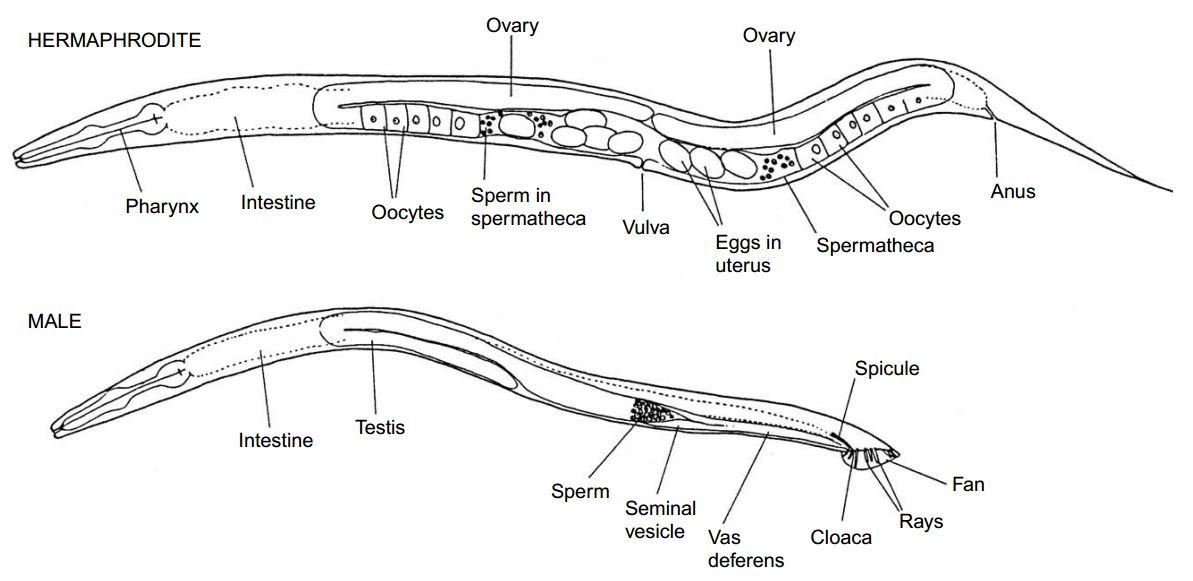
\includegraphics[width=14cm]{figure/chap1/Celegans.jpg}
	  % \hspace{1cm}
	  % 
\includegraphics[width=4cm]{example/sjtulogo.jpg}
	  \bicaption[这里将出现在插图索引中]
		{秀丽隐杆线虫解剖图}
		{Anatomy of adult C.elegans.}
	  \label{fig:Celegans}
	\end{figure}
	秀丽隐杆线虫(简称 C. elegans)是一种微米尺度的无脊椎模式生物,主要生活在土壤中或水中,以大肠杆菌OP50为食,成虫
	体长约为1mm宽度50um,并且从幼虫长到成虫只需要3天。秀丽隐杆线虫是线虫动物门中的一种,包含雌雄同体和雄性两种性别如图\ref{fig:Celegans}。两种性别都是二倍体,都有五对常染色体,
	但雌雄通体的线虫有两个X常染色体(XX)而雄性线虫只有一个X常染色体(XO)。在自然条件下,线虫几乎都为雌雄同体,
	雄性个体只占约五百分之一。线虫的生命周期较为简单如图\ref{fig:lifecycle}所示,成年雌雄同体线虫同时含有精子和卵母细胞,因此能够自体受精。
	每一个自体受精的雌雄同体线虫大约可以产生330多个蛋。如果雄性体线虫交配产蛋量将会提高,并且有利于
	基因的重新组合。在25$^。C$下孵化12个小时即可得到L1期的线虫幼虫,
	长度约为0.15mm。L1期幼虫基本上具备了和成虫一样的器官结构,除了还没有形成生殖器结构,从L1期线虫
	长到L4期只需要3天。
	线虫作为一种现代动物模型被广泛地用于细胞生物学、神经科学、衰老与发育和毒理学等研究中。在2002年
	,研究秀丽线虫的研究团体就已经扩展到300多个实验室,分布在20多个国家和地区。1998年,构成整个基因组的9700万个碱基对DNA的测序基本完成,
	这是第一个经过完整基因组测序的多细胞生物。与其他模式生物相比线虫具有如下技术优势:
	
	\begin{itemize}
	  \item 由于线虫通体透明,可以通过荧光蛋白标记的表达观察细胞的分裂等许多重要的生理过程,
	  还可以用于对神经元成像,研究外部刺激与神经元活动之间的关联。
	  \item 线虫的生命周期短、培养简单以及繁殖能力强,这些特性都有助于加快实验周期,提高实验的并行性。
	  \item 线虫身体构造简单,遗传模式保守,有利于减小实验中由于个体差异而引起实验结果的扰动。
	  \item 对线虫基因的测序已经完成,使得线虫可以在基因筛查分析和其他遗传学实验中发挥重要作用。
	  \item 线虫基因与人类的基因有约40\%的同源性,许多的研究者将线虫作为疾病模型研究疾病机制。
	\end{itemize}
	

	\begin{figure}[h]
	  \centering
	  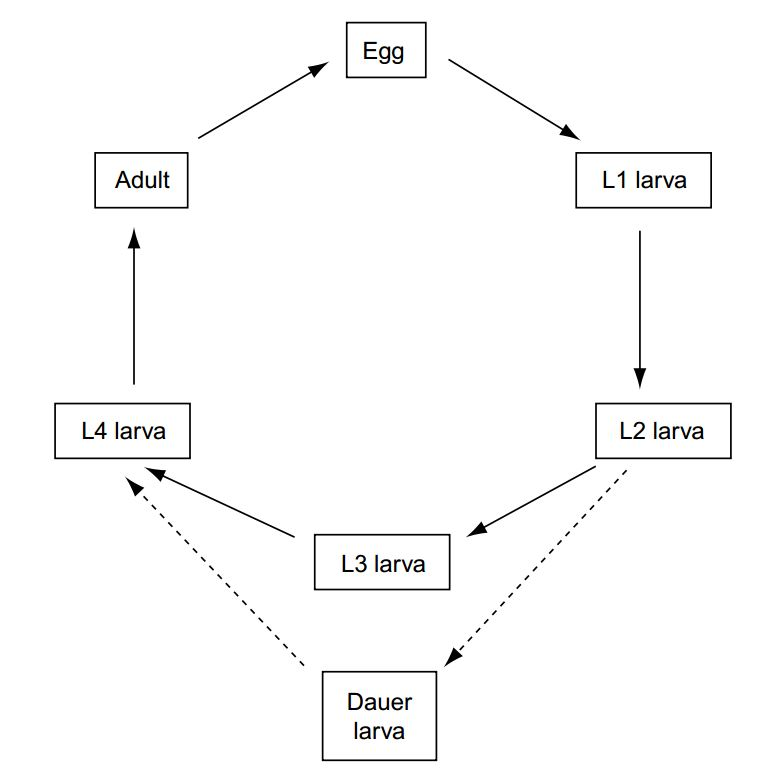
\includegraphics[width=8cm]{figure/chap1/lifecycle.jpg}
	  % \hspace{1cm}
	  % 
\includegraphics[width=4cm]{example/sjtulogo.jpg}
	  \bicaption[这里将出现在插图索引中]
		{秀丽隐杆线虫生命周期}
		{The life cycle of C.elegans.}
	  \label{fig:lifecycle}
	\end{figure}
	
\section{国内外研究现状}
\label{sec:intro:analog}
	微流控是一种在微米尺度操纵流体的技术,具有反应体系小、通量高、自动化且操作灵活等优势,被越来越多的应用于细胞和微米尺度生物的研究中。
	微流控技术在线虫研究中的应用为研究者们提供了一个全新的研究平台,极大的促进了相关领域的研究进展。利用微流控技术研究线虫具有的
	优势有:\begin{enumerate*}[label=\itshape\alph*)\upshape]
	\item 利用微流控芯片可以实现在细胞尺度上对线虫的操纵。\quad
	\item 利用微流控芯片可以实现对线虫的快速固定与成像,与使用药物麻醉的方法相比,这种固定
		方式不会对线虫产生任何损害,线虫可以在后续步骤中恢复。\quad
	\item 利用微流芯片可以快速的从上千只线虫中的筛选出需要的表型,实现线虫的分选。\quad
	\item 微流控芯片可以为线虫的培养提供精确的微环境,为线虫的感知实验提供精确的刺激传达。\quad
\end{enumerate*}
	本文将从以下几个方面对近年来国内外相关领域的发展状况进行回顾,包括线虫的分选、线虫固定与成像以及介绍微流控在毒理学实验中的研究进展。
	最后介绍近年来线虫图像处理的研究进展。
	
\subsection{微流控芯片线虫操控方法}
	在线虫的实验中,经常涉及一些对线虫的日常操纵。如线虫的片上培养、线虫分选、线虫的固定与成像等。
	为了避免复杂的人工操作,研究者们提出了许多不同用途的芯片,这些芯片能够将不同的操作集成在一起,极大的
	提高了实验的并行性和自动化程度。
	
\subsubsection{线虫的培养}
\label{sec:intro:analog}
	线虫的长期培养是研究线虫的衰老和发育的基础,在许多需要对线虫进行长期观察的实验中也需要解决线虫的长期培养问题。
	线虫的长期培养需要与外部环境进行物质交换,包括氧气和食物的供应以及将废物排出。微流控芯片的制作材料一般为聚二甲基硅氧烷
	(ploydimethylsiloxane, PDMS),这种材料具有很好的透气性,因此微流控芯片可以为线虫提供氧气。其中一个早期的工作是由Kim等人\cite{Kim2007Automated}
	完成的,他们设计了一款类似于CD形状的微流控芯片可以实现线虫的片上培养长达数天。食物会在离心力的作用下进入到线虫的培养腔室。
	线虫腔室中的废物会在离心力的作用下被甩出,从而实现了物质的交换。这款芯片可以将线虫培养到三代并且不会影响到线虫的
	生长和行为。然而,由于其芯片结构设计较为简单,所以无法区分不同代之间的线虫且不能实现对单个线虫的跟踪和
	成像。
	\begin{figure}[h]
	  \centering
	  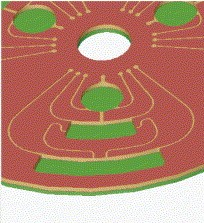
\includegraphics[width=8cm]{figure/chap1/cd.jpg}
	  \bicaption[这里将出现在插图索引中]
		{CD状线虫培养芯片}
		{The life cycle of C.elegans.}
	  \label{fig:cd}
	\end{figure}
	
	由于以上的局限,Hulme等\cite{Hulme2010Lifespan}设计了一款新的芯片。由一排平行的腔室组成,可以实现线虫
	的长期培养及研究其运动行为。利用侧边的楔形通道来固定线虫可以实现线虫的固定与成像以及监测其体长的变化。
	可以同时培养16条成虫,极大的加快了衰老相关的研究,并发现线虫的摆动频率会随着线虫发育日渐成熟而出现下降。
	另一方面,研究者们将液滴和可逆凝胶运用在线虫的长期培养中\cite{Aubry2015Hydrogel,Krajniak2010Long,Wen2015A,Cornaglia2016Automated}。
	Krajniak 和 Lu\cite{Krajniak2010Long}开发了一款集成微流控芯片,该芯片由8个微腔室构成,通过周围的微管道和阀门控制。成功地
	展示了在一块芯片上进行线虫地培养、固定与成像等操作。线虫由一个入口通道进入到8个线虫培养腔室,并将PF127
	可逆凝胶经入口通道注入到线虫培养腔室。这种聚合物在低温(大约15$^\circ$C)下呈现较高地粘性,
	在高温下(大约21$^\circ$C)呈现胶状。运用这款芯片,成功实现了从L1期线虫到成虫过程的生理监测。
\subsubsection{线虫的固定}
\label{sec:intro:analog}
	线虫的固定对于线虫神经元成像与显微手术\cite{Gokce2014A}等需要固定线虫的实验是至关重要的。传统的线虫固定方法经常使用胶水或者麻醉剂
	来固定线虫,使用胶水固定线虫往往很难在短时间内恢复,而使用麻醉剂对线虫神经元可能产生潜在的影响。因此,为了
	实现可逆的无损伤的固定线虫,研究者提出很多基于微流控固定线虫的方法。Chokshi等人\cite{Chokshi2009CO2}开发了一款简单的
	微流控芯片可以有效的固定线虫,并运用这款芯片研究了线虫的运动行为。作者比较了两种不同的固定方法,第一种方法是在上层
	PDMS通道中通入二氧化碳,利用PDMS材料的透气性,上层二氧化碳会向下层扩散从而达到固定线虫的目的;第二种方法是在上层通道
	中施加一个大的气压,从而使中间的PDMS模形变,从而可以将线虫固定。作者还通过评估线虫的运动速度来量化两种不同的固定方式
	对线虫产生的影响,他们发现通过二氧化碳方法固定线虫比用机械的方法固定对线虫的影响较小。
	
	以上的方法虽然能够对成虫进行固定,但由于幼虫的尺寸比成虫小且L1期的幼虫很容易
	将微通道阻塞,因此幼虫的固定是个难点。Aubry等人\cite{Aubry2015Hydrogel}运用FP127凝胶液滴将L1的幼虫包裹,当液滴进入到存储单元
	时可以调整温度从而固定线虫,成功实现对L1期幼虫的操纵及成像。为了研究线虫胚胎发育及其分子机制,Cornaglia
	等人\cite{Cornaglia2015An}设计了一款可以固定线虫胚胎并对其成像的微流控芯片。其由一个线虫培养腔室和许多个微小的胚胎腔室阵列组成,
	研究者可以在胚胎腔室中固定线虫胚胎并且实时观察胚胎发育的整个过程,这种阵列式的腔室结构支持同时对多个线虫
	胚胎进行观察,具有高通量的优势。还有一些研究者利用狭窄的微通道来固定线虫\cite{Lee2014A,Hulme2007A},通过对线虫的存活率和子代的数目
	进行统计发现这种固定方式对线虫没有产生明显影响。
\subsubsection{线虫的分选}
\label{sec:intro:analog}
	目前,使用正向和反向基因筛查的方式筛选新的基因是理解分子通路和蛋白功能的一种非常有效的方法。而在成百上千
	的线虫中筛选出特定表型的线虫是一件耗时且工作量很大的事情,运用微流控器件可以极大的缩短筛查的时间并可以很快
	对观察到的基因变种进行分选。线虫分选芯片的操作往往是基于线虫某种表型的特性如趋电性、行为表型、尺寸、
	运动能力以及电生理学特性的不同等。Rezai\cite{Rezai2012Electrical}等人利用线虫的趋电性设计了一种单层微流控芯片,可以有效的分选出不同
	发育阶段的线虫以及具有神经缺陷的变种。Casadevall\cite{Casadevall2011High}等人设计了一款芯片可以对不同尺寸的线虫同步化,并且可以实现
	每分钟200-1200条线虫的分选速率。Dong\cite{dong2016versatile}等人设计了一种双层的基于PDMS膜形变的线虫分选芯片。通过控制上层气压使
	下层流道层的尺寸发生改变从而只允许特定尺寸的线虫通过这些通道进入另一个腔室。这种方法需要对特定尺寸的线虫
	精确控制施加气压的大小,这款芯片可以以每秒3.5个线虫的速率进行分选。
	% \label{sec:intro:analog}
	% 
	% 可从以下角度分类。
	% \begin{itemize}
	  % \item 有许多文献基于线虫的大小从而对幼虫和成虫进行分选。
	  % \item 线虫的趋电性的不同导致线虫向不同的电极靠近从而达到分选的目的,文献若干。
	  % \item 基于神经元活动和电生理特性的筛选。
	  % \item 区别于物理固定和可逆凝胶固定线虫,研究者提出了一种将液滴捕获用于线虫的分选。
	% \end{itemize}

\subsection{药物筛选与毒理实验}
\label{sec:intro:analog}
	线虫作为一种重要的模式生物与人类的疾病基因具有约65\%的相似性\cite{Baumeister2002The,Sonnhammer1997Analysis},
	因此线虫在药物筛选和毒理学研究领域经常作为一种重要的研究对象。近年来,研究者们设计了很多用于实时药物
	识别、筛选和毒性测试的微流控芯片。Chung等人\cite{Chung2011Microfluidic}开发了一款包含48个平行阵列腔室的微流控芯片,每一个腔室单元的
	直径为1.5mm,并且还设计了一条宽500um的管道用于将线虫和化合物送到每个腔室。所有的腔室在视野种都是可见的,因此
	便于观察每个腔室中单个线虫暴露在某种化合物下的反应。Yang等人\cite{Yang2013An}开发了一款双层的可以评估体内抗菌活性的微流控芯片,
	芯片呈现放射状四周分布着32个腔室,中心有一个存储的腔室,有四个“圣诞树”结构的片上浓度梯度生成器\cite{Dertinger2001Generation,Jeon2000Generation}。利用
	这款芯片可以同时研究4种药物32种浓度梯度对线虫的影响。中科院大连化学物理研究所设计制作了一种三夹层的芯片,
	该芯片由上层液路层、中间气路控制层和底层玻璃组成。液路层有30个长2mm$\times$宽1mm$\times$厚70um的线虫
	培养腔室用于线虫培养何成像,中间有一个废液池用于收集线虫培养腔室中的废液。并应用该芯片探究了高糖对线虫
	寿命的影响\cite{zhuliguo2016}。
	% 很多的线虫芯片被开发,用于药物识别,筛选、以及研究毒性对线虫行为、生理电信号衰老。抗菌和代谢
% 活动身体毒性的影响。
	% \begin{itemize}
	  % \item 多种复合药物浓度梯度的药物筛选。
	  % \item 将线虫暴露在细菌病原体环境中。
	  % \item 将线虫暴露在重金属环境中
	% \end{itemize}
	
\subsection{机器视觉在线虫研究中的应用}
\label{sec:intro:analog}
	研究线虫的运动行为并对其量化在许多线虫研究中(如:神经学、遗传学和毒理学等研究中)起着十分重要的作用,
	通过人工观察不仅效率低下而且还会引入人为误差,如在基因筛查中需要在成百上千的线虫发现行为异常的线虫往往
	需要分析几百个小时的视频,因此应用机器视觉的方法量化运动相关的表型具有重要的意义。近年来,研究者们提出
	很多自动化线虫图像处理的方法。Dhawan等人\cite{De1998Natural}设计一个可以在较低的倍率同时跟踪多个线虫的系统,
	但是该系统只能得到线虫运动方向等信息,无法得到线虫形态和姿势等相关特征(如体长、运动速度等)。
	Baek等人\cite{Baek2002Using}开发了一个可以在较高倍率下跟踪单个线虫的系统,通过控制载物台的移动可以
	保证线虫始终出现在视野中,通过提取94种不同的特征并利用决策树对特征向量进行分类可以区分出行为异常的线虫变种。
	在2011年,剑桥大学分子生物学实验室研究人员设计了一款名为Wormtracker的系统,该软件可以包含一套定制的软硬件
	系统\cite{yemini2013high}。与之前的单线虫跟踪系统相比,可以将成本下降四分之一,该系统另一个优点是能够实现对所有发育阶段的幼虫
	的跟踪以及游动状态下单线虫的跟踪。Swierczek等人\cite{swierczek2011high}设计了一款名为
	Multi-Worm Tracker(MWT)的软件,最多可以实现对120条线虫的跟踪,但只能以离线的方式对采集到的
	视频数据进行特征提取无法实现特征的实时提取。另外,当多个线虫的相遇并相互遮挡时,系统只会识别到一个轮廓,
	这样会导致跟踪的失败。
	
	为了解决线虫跟踪过程中线虫轮廓的重叠与遮挡的问题,研究者们提出了一些基于模型的跟踪算法。Restif等人\cite{restif2008tracking}
	提出一种针对游动线虫的跟踪算法。其将线虫的跟踪分成两个阶段:第一个阶段是通过线虫轮廓运动的历史状态预测下个状态
	线虫轮廓运动的速度,结合当前状态下线虫轮廓的位置可以计算出下个时刻线虫轮廓出现的位置;第二个阶段主要是
	调整上个阶段得到的线虫轮廓使其与图片上线虫的轮廓重合。 Fontaine和Roussel等人\cite{fontaine2007model,roussel2014robust}提出了一种
	可以对线虫和斑马鱼进行跟踪的算法,其主要思想是通过对线虫轮廓进行参数化建模得到状态空间并通过
	迭代卡尔曼滤波器来预测模型参数从而实现线虫的跟踪。针对单个线虫发生自身卷曲时其轮廓识别的困难,Nagy等人
	\cite{nagy2015generative}提出一种基于统计生成式方法可以识别复杂的姿态。
	
	线虫的图像处理一般分为两个模块,分别是线虫的跟踪(包括线虫轮廓的分割)和线虫的特征提取。线虫的跟踪模块
	主要是得到线虫的轮廓,线虫的特征提取模块是利用跟踪到的线虫轮廓进行特征计算。Yemini等人\cite{yemini2013database}
	对线虫相关的行为表型进行了综述并将其分为四大类:分别为形态特征(如:体长、体宽和面积等)、姿势特征(如:
	线虫脊线的水平投影长度、波长以及弯曲的数量等)、运动特征(如:运动速度和运动状态等)、轨迹特征(如:线虫重心
	移动轨迹的范围和轨迹图等)。线虫姿态的描述一般是通过在线虫的中间脊线上等距的采样固定数量的点来定义的。
	这样得到线虫姿势的状态空间通常是很大的,Stephens等人\cite{Stephens2008Dimensionality}提出一种降维的方法
	从而可以在较低的维度空间描述线虫的姿势状态。其主要的思想是计算线虫中间脊线的曲率从而得到一个曲率向量,
	并对其归一化然后计算这个向量的协方差矩阵,发现其大部分的特征值为零。作者取了四个最大的特征值对应的
	特征向量作为四个本征向量,这四个本征向量将构成一个状态空间,任何线虫脊线曲率向量都可以投影到这个空间。
	由此得到四个投影长度即可描述线虫的姿势。即可以在一个四维空间中描述线虫的姿势。Restif等人\cite{Restif2014CeleST}提出了一种新的
	计算特征的方法。通过将计算同一个线虫的脊线曲率向量并将其按照时间顺序排列,由此即可得到一个矩阵。通过
	对这个矩阵做二维离散傅里叶变换。最后基于傅里叶变换的结果计算线虫相关的特征。为了实现线虫行为数据的
	共享,Javer等人\cite{Javer2018An}提出统一的数据格式支持对视频数据以及对应的特征数据的读取以存储。
	并定义了一种中间数据格式表示Worm tracker Commons Object Notation (WCON)这样可以方便研究者组合使用不同
	线虫跟踪模块和特征提取模块。
\section{存在的问题}
\label{sec:intro:analog}
	\begin{itemize}
	  \item 片上梯度的形成
	  \item 游动线虫轮廓的分割
	  \item 一个集成微流控芯片和多线虫实时图像处理的平台还报道的比较少
	\end{itemize}
\section{研究内容}
\label{sec:intro:org}
	\begin{itemize}
	  \item 首先搭建了一个基于微流控芯片的硬件平台
	  \item 设计了一款及线虫轮廓分割、跟踪及特征提取等功能的自动化图像处理软件。
	  并针对线虫分割的鲁棒性与实时性的要求,还提出了一种基于深度学习的线虫轮廓分割的网络。
	  \item 在搭建的硬件平台上,并通过双氧水实验验证 系统的优势。
	\end{itemize}
\section{论文章节安排}
\label{sec:intro:org}

\chapter{微流控线虫芯片的设计及硬件平台的搭建}
\section{引言}
	
	在传统的药物筛选过程中,往往是通过人工的方式在96孔板上配置不同浓度的化合物。
	然后将线虫暴露在不同浓度的化合物下,观察并记录线虫在不同浓度化合物下的变化。
	这种人工稀释的方法不仅存在样品消耗大、通量低和操作繁琐等缺点,而且也不利于
	观察。近年来,随着微流控技术的发展,一些研究者们提出了基于微流控技术的片上浓度稀释的方法。
	片上浓度梯度稀释的方法不仅使反应体系减小十倍甚至百倍,
	而且极大的减少了试剂的消耗,节约了实验成本。虽然已经有“圣诞树”结构的被动式梯度
	形成芯片的报道,但存在样品消耗大以及需要精确的流阻设计和流速调节。
	为了研究多种化合物的复合对线虫活性的影响,
	本文设计了一种基于振荡的线性梯度稀释的微流控芯片。且只需要一个气源即可通过振荡的方式
	完整样品的快速稀释,并通过染料实验和荧光实验验证本文提出的线性浓度梯度芯片的可行性。
	
\section{双层线虫梯度芯片的设计及制作}
\subsection{线虫梯度芯片的设计}
\label{arch-design}
\begin{figure}[htbp]
	  \centering
	  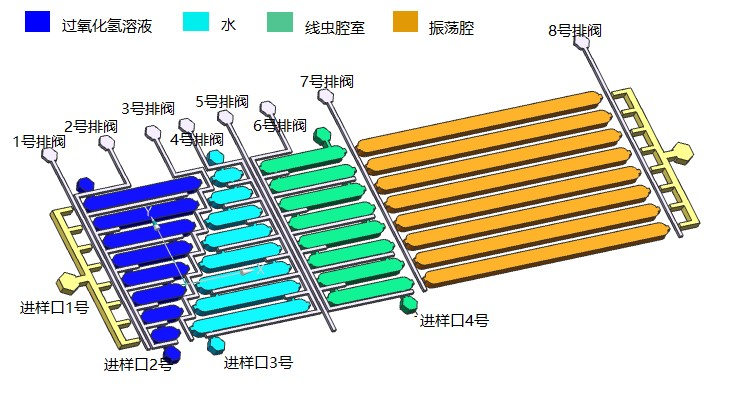
\includegraphics[width=13cm]{figure/chap2/chip-arch.jpg}
	  \bicaption[这里将出现在插图索引中]
		{线性梯度稀释芯片结构}
		{Structure of Linear gradient dilution chip}
	  \label{fig:chap2:chip-arch}
	\end{figure}
线虫梯度芯片的设计如图\ref{fig:chap2:chip-arch}所示,由两层PDMS管道组成。上层为流道层,下层为阀门层。
芯片包含八个阀门和四个进样口。阀门分别控制每列之间的隔绝和开启以及每列腔室之间的相互隔绝和开启。
其中3、5、7号阀门控制4列每列之间的隔绝,而2、4、6号阀门分别控制1、2、3列里9排腔室之间的隔绝,8个阀门将整个芯片分为$9\times4$个独立的腔室。
4列腔室中第一列腔室的长度依次线性递减,第二列腔室的长度依次线性增加,前两列腔室的长度总和为2mm (两腔室长度的比例从上到下依次为$9:1,8:2,\dots,1:9$)。
第三列和第四列腔室的长度保持恒定分别为1mm和3mm。所有腔室的宽度和高度分别为200um和80um。

\subsection{实验材料与仪器}
	\begin{table}[htbp]
	\centering
	\bicaption[指向一个表格的表目录索引]
    {实验试剂与耗材}
    {Experimental reagents and consumables}
	\begin{tabular}{p{150pt}p{230pt}}
	\toprule
		光刻胶SU-83050 & 美国Microchem公司\\
		光刻胶AZ4903 & 德国Merck Performance Materials公司\\
		聚二甲基硅氧烷PDMS( polydimethylsiloxame, RTV 615) &美国 Momentive Performance Materials 公司\\
		氟化液FC-40 & 北京伊诺凯科技有限公司\\
		FA1004分析电子天平 & 上海良平仪器仪表有限公司\\
		RC8型匀胶机 & 美国 Karl Suss公司\\
		DZF-6020型真空干燥箱& 上海新苗医疗器械制造有限公司\\
		ZXZ-2型旋片式真空泵 & 浙江谭氏真空设备有限公司\\
		SMZ-168型体式显微镜& 中国麦克奥迪公司 \\
	\bottomrule
	\end{tabular}
	\end{table}
\subsection{芯片模具加工工艺}
\subsubsection{阀门层模具制作}
	
	\begin{enumerate}[label={\alph*)},font={\color{black!50!black}\bfseries}]
	\item 按照\ref{arch-design}小节的结构设计使用AutoCAD绘图软件绘制阀门层的结构图案并制作掩模版。
	\item 在涂胶之前,需先将3英寸的单抛硅片放在180$^\circ C$的烘箱中2小时,然后用氧等离子体去胶机处理60秒。
	\item 旋涂光刻胶AZ4903并用200rpm的转速预转8秒,然后再用1000rpm的转速甩胶25秒得到22um厚的胶。
	\item 将硅片放入烘箱中,逐渐升温至$50^\circ C$,30分钟后再将温度升高至$90^\circ C$,90分钟后再将其取出。
	\item 经过紫外曝光后再显影。
	\item 为了去除硅片表面的水汽,将其放入$80^\circ C$的烘箱中1小时,最后使用甲基三氯硅烷处理硅片表面5分钟。
	\end{enumerate}
	
\subsubsection{流道层模具制作}
	由于本文中芯片的管道和腔室的高度被设计成不同的尺寸,且腔室的高度要比管道的高度要高,
	所以需要经过两次光刻才能完成流道层模具的制作,第一次光刻采用正胶制作管道结构,第二次光刻采用负胶制作腔室结构。
	\begin{enumerate}[label={\alph*)},font={\color{black!50!black}\bfseries}]
	\item 使用AutoCAD绘图软件分别绘制芯片管道和芯片腔室的结构并打印制作掩模。
	\item 在涂胶之前,需先将3英寸的单抛硅片放在180$^\circ C$的烘箱中2小时,然后用氧等离子体去胶机处理60秒。
	\item 旋涂光刻胶AZ4903并用200rpm的转速预转8秒,然后再用1000rpm的转速旋涂25秒得到22um厚的胶。
	\item 将硅片放入烘箱中,逐渐升温至$50^\circ C$,30分钟后再将温度升高至$90^\circ C$,90分钟后再将其取出。
	\item 经过紫外曝光后再显影。
	\item 将硅片放在热板上分别升高温度分别在$65^\circ C$、$95^\circ C$、$120^\circ C$和$190^\circ C$分别停留
	5min、5min、40min和60min。
	\item 旋涂负胶SU-8 3050并用500rpm的转速预转8秒,然后再用1500rpm的转速旋涂30秒得到80um厚的胶。
	\item 将硅片放在$95^\circ C$的烘箱中恒温40min。
	\item 经紫外曝光后将硅片放入$95^\circ C$的烘箱中恒温60min。
	\item 用对应的显影液对硅片显影,并用异丙酮溶液漂洗,以除去残留的显影液和试剂残留并用氮气将硅片吹干。
	\item 为了除去水汽,将硅片放入$80^\circ C$的烘箱中恒温60min,再用甲基硅氧烷处理5min。
	\end{enumerate}
\subsection{线虫梯度芯片的制作}
	制作好芯片模具后,就可以利用芯片模具进行微流控芯片的制作,下面将介绍双层微流控芯片的制作流程。经过以下流程
	最终完成的芯片其实物图如图\ref{fig:chap2:chip-fabric}所示,为了更好的显示芯片结构,芯片的四列腔室
	都被打入不同颜色的染料。
	\begin{enumerate}[label={\alph*)},font={\color{black!50!black}\bfseries}]
	\item 将流道层硅片的背面用胶粘在一次性培养皿的底部,起到一个固定的作用。
	\item 配制PDMS:按照20:1的比例,取20克RTV 615(A液)和1克固化剂(B液)混合搅拌均与,按照5:1的比例,
	取20克RTV 615(A液)和4克固化剂(B液)混合搅拌均匀,并将两种比例的混合液放入真空皿中抽真空以排出液体中的气泡,
	不断地抽气放气直到液体呈现澄清状。
	\item 将5:1的PDMS混合液倒入流道层培养皿中,PDMS混合液的厚度大约5mm左右。
	\item 将阀门层硅片放在甩胶机吸盘的中心位置,并用真空吸住硅片使其固定,将20:1的PDMS混合液倾倒在硅片上,
	用400rpm的转速预转20秒后再用1800rpm的转速转60秒即可得到厚约40um的PDMS层。
	\item 将阀门层模具和流道层模具一起放入$80^\circ C$的烘箱中恒温30min。
	\item 用手术刀将培养皿中的PDMS层沿着硅片的边沿切下并取出。再用铲刀沿着芯片上的图案将其切成长方形。
	\item 在显微镜下将上一步切下的流道层芯片与阀门层对准并粘合在一起。
	\item 将其放入$75^\circ C$的烘箱中恒温5个小时进行高温键合,然后将其取出放在无尘纸上进行常温冷却。
	\item 再用打孔器将芯片的进样口、出样口和阀门入口位置打孔。
	\item 将芯片和干净的玻璃片一起放入氧等离子体去胶机中处理40秒后,将芯片和玻璃贴合在一起并放入$80^\circ C$的烘箱中
	恒温2小时。
	\end{enumerate}
	\begin{figure}[htbp]
	  \centering
	  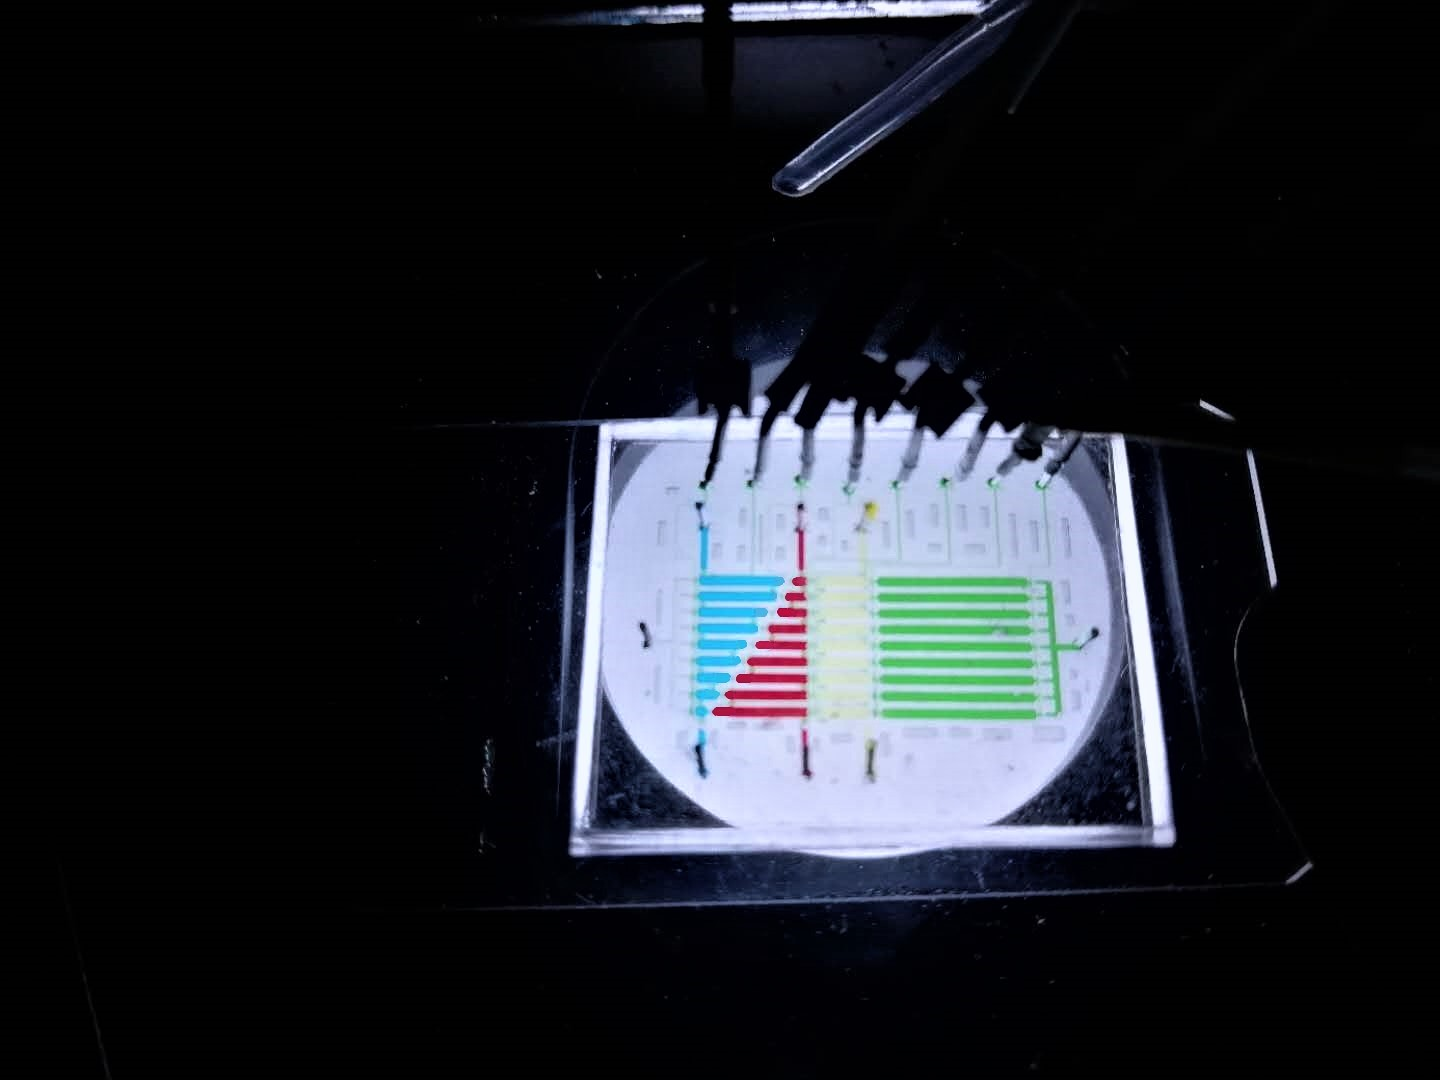
\includegraphics[width=9cm]{figure/chap2/fabric-chip.jpg}
	  \bicaption[这里将出现在插图索引中]
		{线性梯度稀释芯片实物图}
		{fabricated linear gradient dilution chip}
	  \label{fig:chap2:chip-fabric}
	\end{figure}
\subsection{振荡的理论机制}
	在微流控芯片中,流体的雷诺系数Re变得很小,流体以层流的方法流动,
	这使得微管道中的不同液体的混合变得非常缓慢。我们课题组提出了一种只需一个压力源的基于流体振荡的混合器\cite{cheng2018simple},
	振荡的时候需要在管道的一端构造一个封闭的空腔环境。当需要混合前两列腔室中的液体时,需要将第三列作为储气腔,
	将第三列腔室右边的阀门关闭即可形成封闭的储气腔。当需要混合前三列腔室中的液体时可以将第四列腔室作为储气腔。
	振荡的时候将九排腔室之间的阀门关闭,对其中一排腔室的受力分析可等效为图\ref{fig:force},
	其中$P_{atm}$、$P_{push}$和$P_{air}$分别表示大气压、外部施加的压强与大气压的差和储气腔中的气压。
	储气腔由于封闭了一段空气,当开始施加外部压力时,此时外部气压大于储气腔内的气压,
	会推动液体往储气腔运动,储气腔内的气体由于受到液体的挤压,体积会收缩且内部压强开始增大;
	当外部压力撤掉时,由于储气腔中的压强大于外部的压强,液体会向反方向运动,
	这时储气腔的体积会增大压强会变小。当压强下降到等于外部压强时,液体会停止向前运动,继续施加压力,
	液体又会重复上述运动,这样液体会在周期性气压的作用下来回振荡,类似于宏观的混合吹打从而完成不同溶质的混合。
	\begin{figure}[!htp]    
	\begin{minipage}[t]{0.5\linewidth}%设定图片下字的宽度,在此基础尽量满足图片的长宽    
		\centering    
		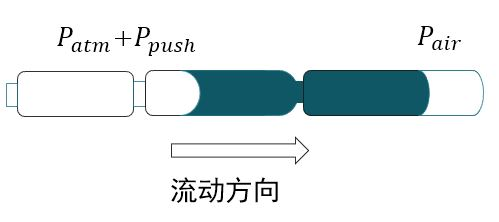
\includegraphics[width=1\linewidth]{figure/chap2/force2.jpg}    
		\caption*{(a) 压缩过程受力分析}%加*可以去掉默认前缀,作为图片单独的说明    
		\label{fig:compress}    
	\end{minipage}    
	\begin{minipage}[t]{0.5\linewidth}%需要几张添加即可,注意设定合适的linewidth    
		\centering    
		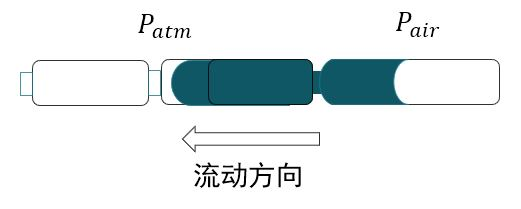
\includegraphics[width=1\linewidth]{figure/chap2/force1.jpg}    
		\caption*{(b) 解压缩过程受力分析}
		\label{fig:decompress}
	\end{minipage}
	\bicaption{液体振荡过程受力分析}{ Stress analysis of liquid oscillation process}%n张图片共享的说明
	\label{fig:force}
	\end{figure}
	
\subsection{染料与荧光实验}
为验证振荡混合效果,我们使用染料及荧光进行验证。如图\ref{fig:before}所示,将第一列腔室打入红色染料,
第二列腔室打入水,将第三列腔室作为振荡腔。在1号进样口施加一个周期为250ms压力值为0.05Mpa的气压,
经过7分钟的振荡,染料已经充分的混合均匀。染料和水完全混合后的效果如图\ref{fig:after}所示,从上到下染料的颜色依次变淡。
如不加振荡,两列液体以自由扩散方式混合,需要2~3个小时,可以看出,振荡方法对快速混合形成梯度有较好的效果,
大大加快了不同液体的混合速率。
为了定量的验证梯度形成的准确性,我们将第一列腔室中的染料替代为浓度为0.1g/L 的荧光素钠溶液(pH=7),
最终得到0.01~0.09g/L的线性浓度梯度。图\ref{fig:chap2:fluence}为荧光素钠浓度与荧光强度之间的关系。
图中蓝色的线表示线性拟合的结果,可以看出拟合结果的线性度较好。
从而验证了基于微振荡原理的大规模梯度稀释是可行的,
这种方式能够显著加快混合的速度并且只需要一个压力源即可完成振荡混合。
为了验证这种振荡对线虫并无不良后果,我们将线虫打入第三列腔室,并在该参数下振荡,
观察2个小时发现线虫的摆动频率并没有出现太大波动。

	\begin{figure}[!htp]
	\centering
	  \begin{subfigure}{0.45\textwidth}
		\centering
		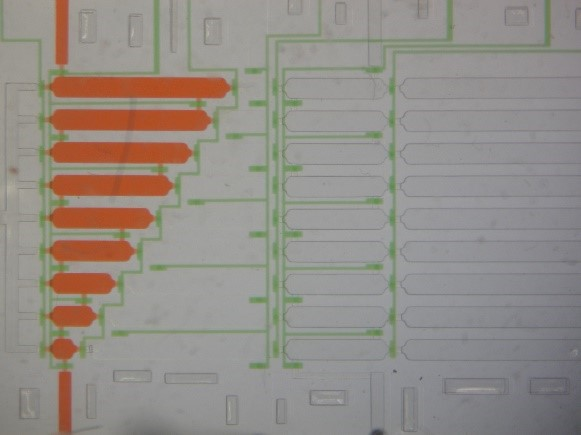
\includegraphics[width=1\linewidth]{figure/chap2/before.jpg}
		\caption{振荡前的芯片图 }
		\label{fig:before}   
	  \end{subfigure}
		\hspace{1em}
	  \begin{subfigure}{0.45\textwidth}
		\centering
		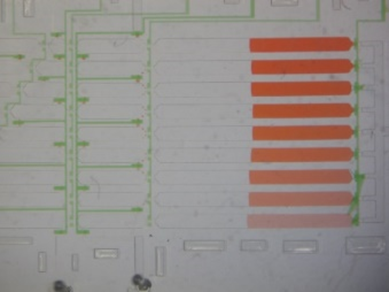
\includegraphics[width=1\linewidth]{figure/chap2/after.png}
		\caption{振荡结束后的芯片图}
		\label{fig:after}
	  \end{subfigure}
	  \bicaption{染料实验结果}{Dye experiment results}
	  \label{fig:oscillation}
	\end{figure}

	\begin{figure}[htbp]
	  \centering
	  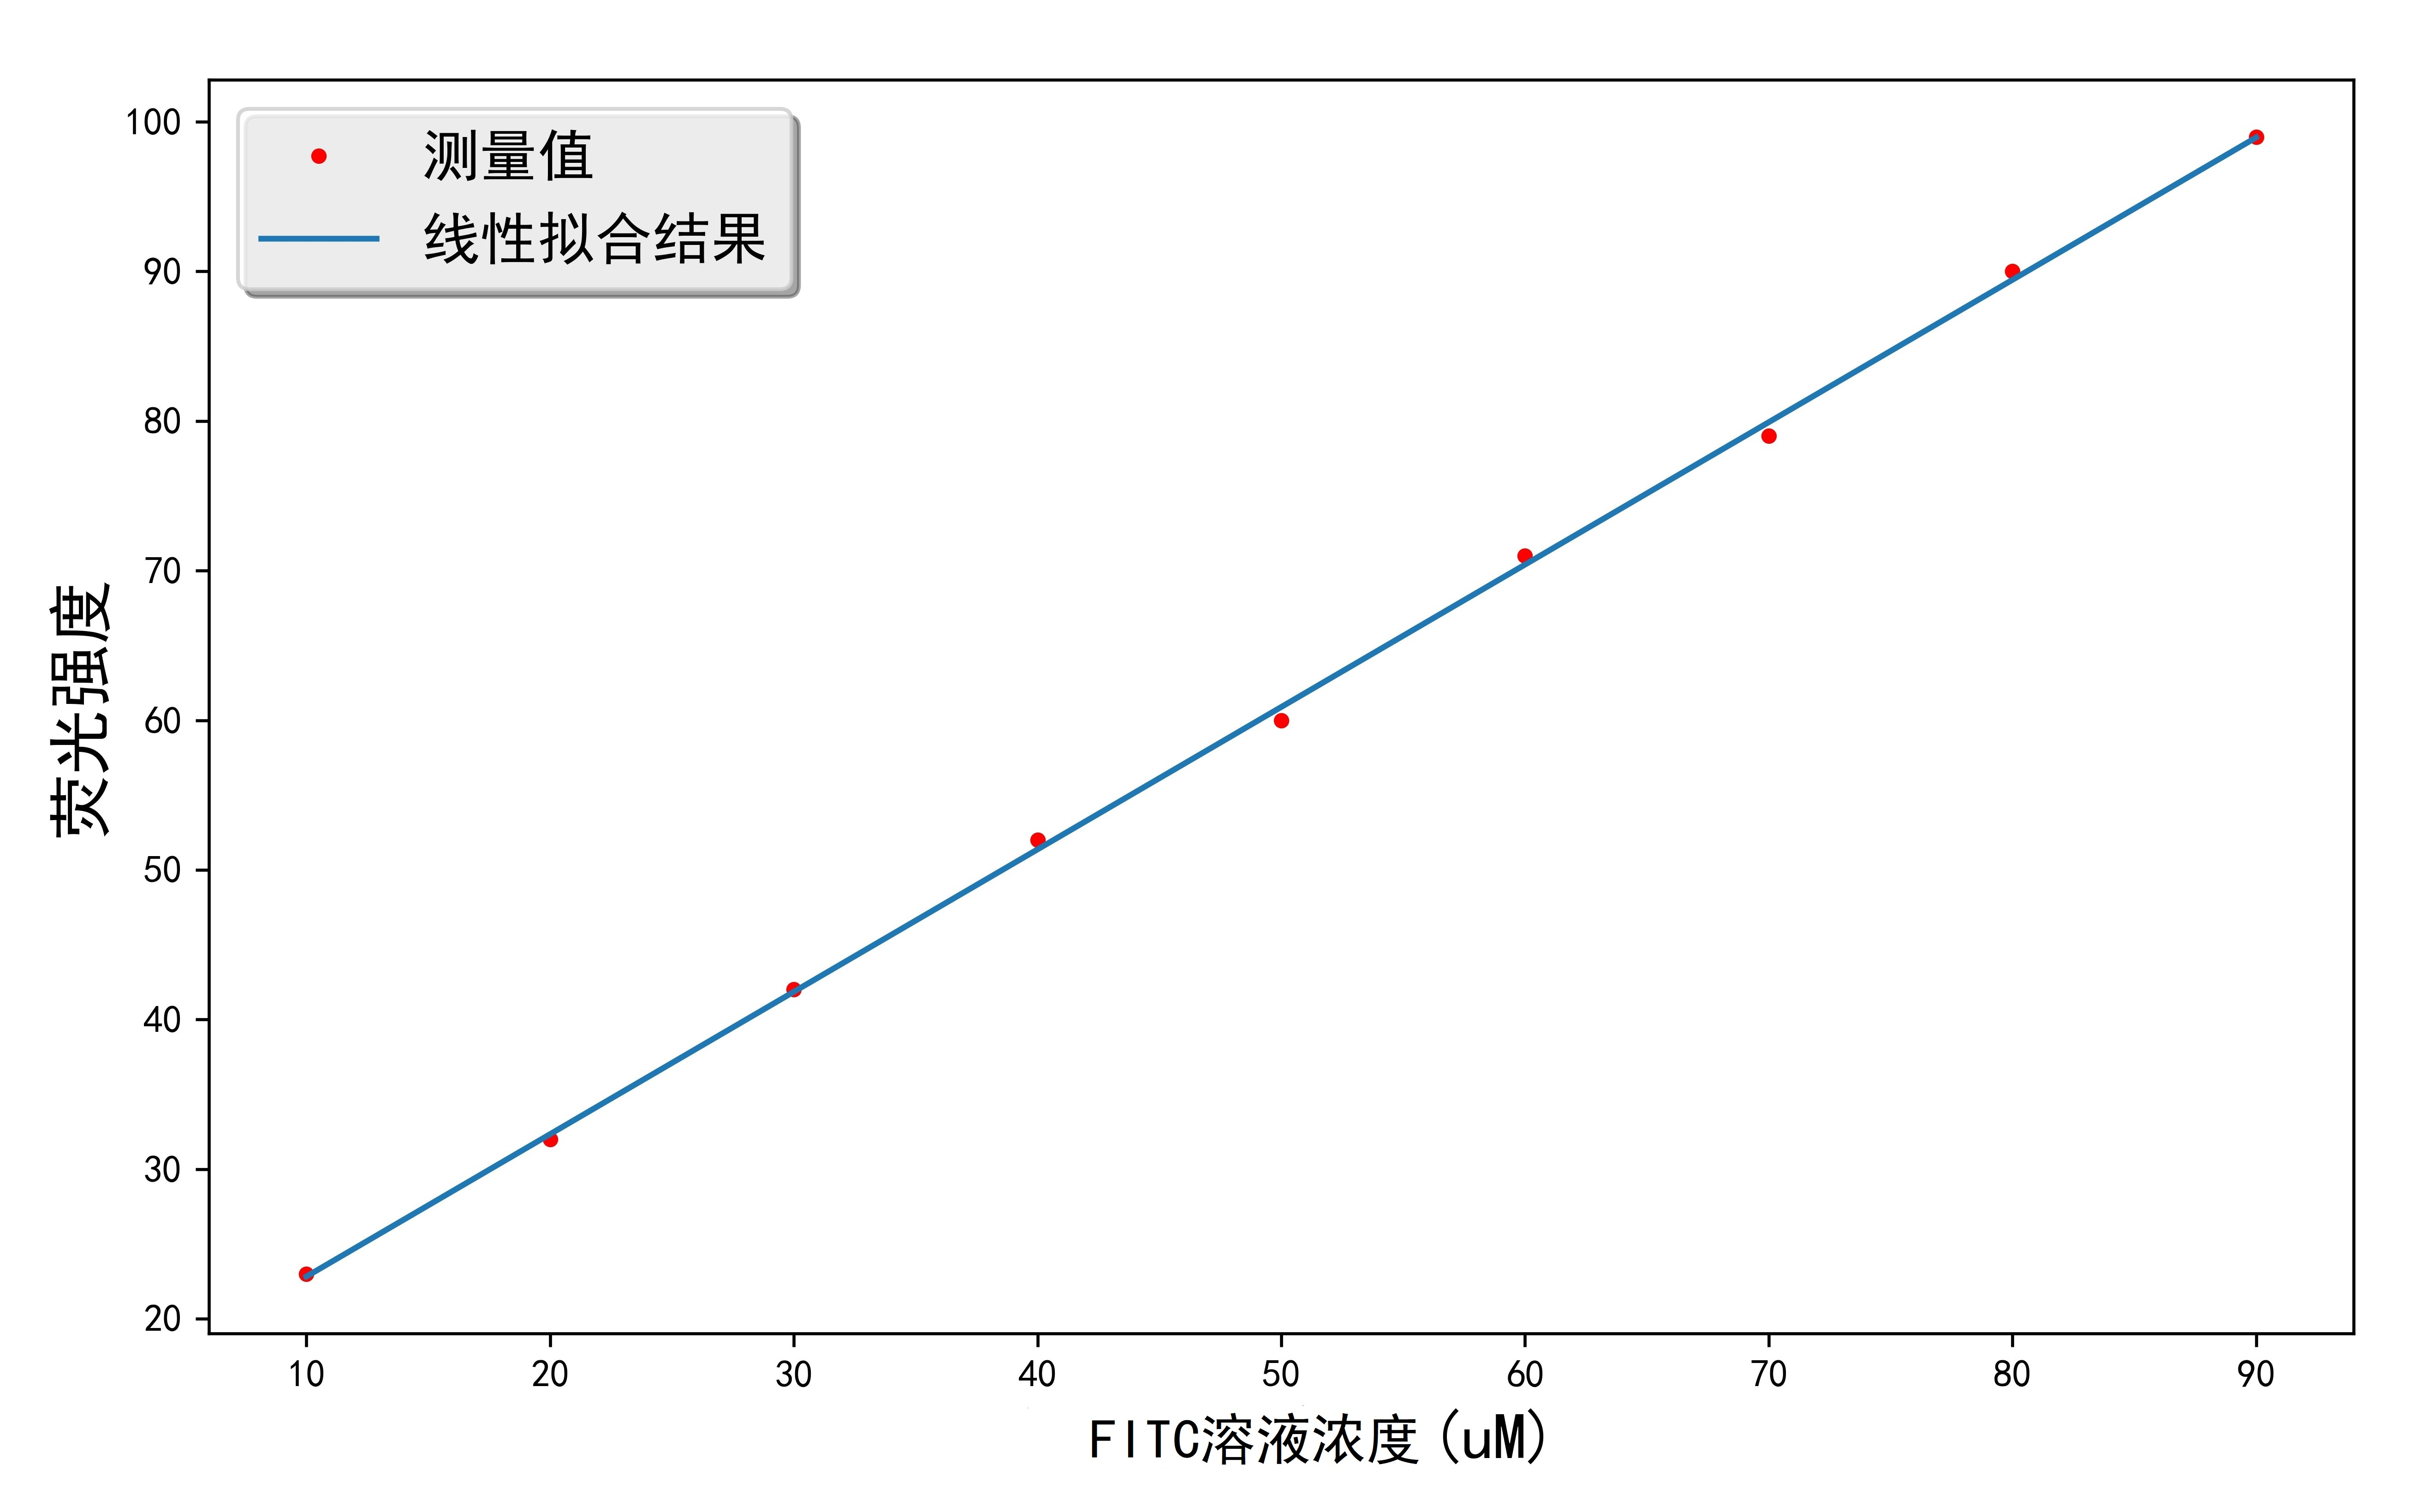
\includegraphics[width=9cm]{figure/chap2/fluence.jpg}
	  \bicaption[这里将出现在插图索引中]
		{荧光实验结果}
		{Fluorescence experiment results}
	  \label{fig:chap2:fluence}
	\end{figure}
\section{单层侧向阀门线虫培养芯片的设计及制作}
\subsection{单层阀门线虫培养芯片的设计}
\label{subsec:chipdesign}
	\begin{figure}[htbp]
	  \centering
	  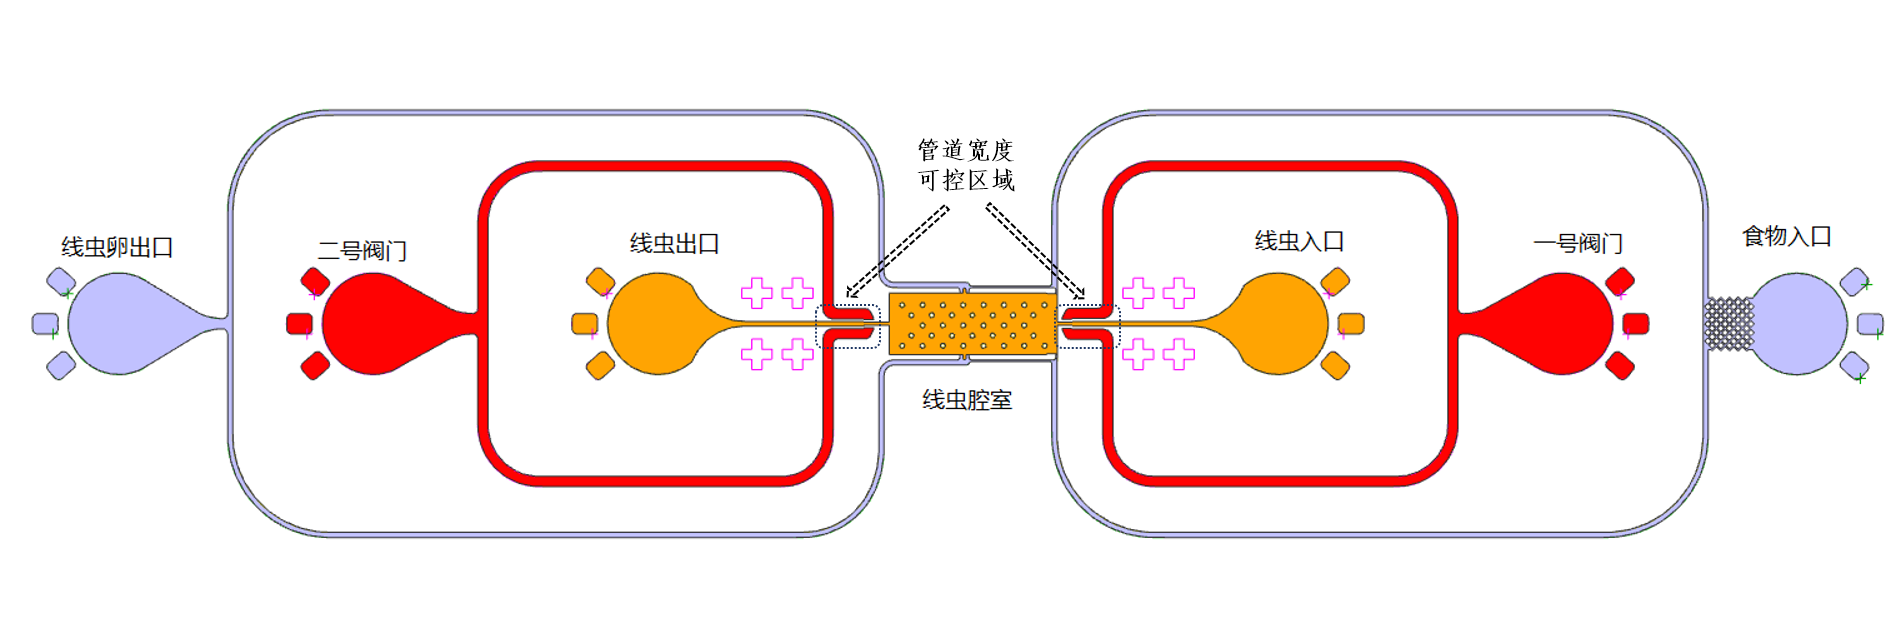
\includegraphics[width=9cm]{figure/chap2/arch-chip.png}
	  \bicaption[这里将出现在插图索引中]
		{单层阀门线虫培养芯片}
		{Single layer lateral valve chip for  worm culture}
	  \label{fig:chap2:fluence}
	\end{figure}
\subsection{单层阀门芯片模具的制作}
	下面开始介绍单层阀门芯片模具的制作工艺流程。
	\begin{enumerate}[label={\alph*)},font={\color{black!50!black}\bfseries}]
	\item 根据芯片结构的尺寸设计运用AutoCAD绘图软件绘制芯片的二维结构并制作掩模版。
	\item 为了使光刻胶和硅片更容易结合,必须充分去除硅片的水分。将单面抛光的3寸硅片放进
	$180^\circ C$烘箱中恒温$2\sim3$个小时。
	\item 将硅片从烘箱中取出,待其恢复到室温后,用氮气将硅片表面的杂质吹掉使硅片表面保持干净。
	用光刻胶AZ-4903倒在硅片的中心出,使其自然铺开慢慢覆盖硅片表面。然后5000rpm的转速旋涂30s得到胶层厚度
	大约为1um。
	\item 为了去除光刻胶中的有机溶剂并使光刻胶固定需要经过前烘,将涂有光刻胶的硅片放入烘箱中。将烘箱的温度
	缓慢升至$65^\circ C$,恒温30min。然后继续将温度升至$90^\circ C$,再恒温30min,最后慢慢将烘箱温度降至
	室温。
	\item 将硅片放入光刻机中,曝光前,先打开光刻机汞灯预热10min分钟。将掩模版放在硅片上面并中心对齐,根据
	光刻机的厚度调整好曝光时间,经过曝光处理后,将可掩模上的图案转移到光刻胶上。
	\item 将经过曝光处理的硅片放入烘箱中逐渐升温至$65^\circ C$并恒温15min,然后再逐渐升温至$95^\circ C$
	恒温40min,最后慢慢将温度降到室温。
	\item 经过后烘步骤,再用对应的显影液对硅片进行显影,得到清晰的图形后再用氮气将硅片表面吹干。
	\item 将硅片放入深硅刻蚀机中,进行干法刻蚀。光刻胶覆盖的区域将不会被刻蚀,从而可以将掩模板上的芯片
	图案转移到硅片表面。注意根据腔室的高度,控制好刻蚀的厚度。
	\item 为了使PDMS芯片的制作过程中,PDMS层容易从模具上揭下来,需要对硅片表面进行硅烷化处理。
	将硅片放入一次性的培养皿中,在硅片旁的滤纸上滴一滴硅烷化试剂,通过蒸发沉淀的方式完成硅烷化处理。
	\end{enumerate}
\subsection{单层阀门芯片的制作}
	将PDMS浇筑在芯片的模具上待其固化,即可完成
	\begin{enumerate}[label={\alph*)},font={\color{black!50!black}\bfseries}]
	\item 将硅片模具固定在一次性的培养皿的底部。
	\item 配置PDMS混合液:按照10:1的比例,取20克的PDMS(Sylgard 184)A液和2克的固化剂(B液)混合搅拌均匀,
	并将两种比例的混合液放入真空皿中抽真空以排出液体中的气泡,不断地抽气放气直到液体呈现澄清状。
	\item 将PDMS浇筑在放有硅片模具的培养皿中,浇筑厚度约为5mm,重新放回真空皿中抽出芯片表面的气泡。
	\item 将培养皿放入$75^\circ C$的烘箱中恒温一个小时使PDMS得以固化。
	\item 从烘箱中取出芯片模具,待其自然冷却,用手术刀将PDMS层从模具上揭下来。按照芯片上的图案用PDMS切成方形,
	并在所有进口、出口处打孔。
	\item 将芯片和干净的玻璃片一起放入氧等离子体去胶机中处理40 秒后,将芯
片和玻璃贴合在一起并放入$80^\circ C$的烘箱中恒温2小时,加强键合效果。
	\end{enumerate}
\subsection{单层侧向阀门线虫固定芯片的测试}

\section{阀门控制系统搭建}
	目前,双层的微流控芯片一般由下层的阀门层和上层的流道层组成。阀门层的PDMS薄膜通常很薄,当向气阀通道施加一定的
	气压(大约30psig),阀门层的薄膜会向上顶起。由于上层的流道和下层的气阀通道是上下交叉的,通过控制向气阀通道施加
	气压,便可以控制上层流道的通断。另一方面,线虫的压力进样和芯片的振荡都需要对进样口进行气压控制。基于以上需求
	,本课题组开发了自动化阀门控制系统,图\ref{fig:flow_chart}为该系统的连接示意图。整个系统由五个模块构成,
	我们采用了750W-18L小型空压机作为气泵模块为整个系统提供气压输出,将Arduino作为微控制器控制电磁阀的输出。
	Arduino由运行在电脑上的上位机程序控制。

	\begin{figure}[!htp]
    \centering
	
    \begin{tikzpicture}[node distance=2.5cm,auto]
	\tikzstyle{process} = [rectangle,rounded corners,thick,minimum width = 3cm,text width=3cm,inner sep=2pt,minimum height =1.7cm, text centered, draw = black]
    \node (pc) [process] {电脑};
    \node (mcu) [process, below of=pc] {微控制器及运算放大器};
    \node (valves) [process, below of=mcu] {电磁阀};
    \node (pump) [process, right of=valves,node distance=4cm] {气泵};
    \node (chip) [process, left of=valves,node distance=4cm] {微流控芯片};
    %连接具体形状
    \draw [arrow](pc) -- (mcu);
    \draw [arrow](mcu) -- (valves);
    \draw [arrow](valves) -- (chip);
    \draw [arrow](pump) -- (valves);
	\end{tikzpicture}
    \bicaption{自动化阀门控制系统}{Automated valve control system}
    \label{fig:flow_chart}
	\end{figure}
\section{高速视频采集程序的设计}
	线虫视频的高速采集对线虫摆动频率的估计是至关重要的一步。根据采样定理,采集的视频帧率至少是线虫摆动频率的两倍。
	除了采样频率的要求外,视频的分辨率等因素同样影响后续线虫图像处理的难度。基于以上考虑,本文选取鑫图公司的DigiRetina 16
	 COMS相机作为线虫视频的采集模块。其可以通过USB3.0高速传输接口与电脑进行高速图像数据传输,同时该相机在放大倍率20
	 倍以下的显微成像中,也可以获得分辨率优异的显微图像,另外其内置两个FPGA双核处理器分别用于高清图像处理和
	 图像输出控制。该相机较好满足了本文对线虫视频采集模块的要求。为了提高视频采集的帧率,本文基于该相机的SDK,开发基于多线程
	 的视频采集程序。
	 
	对DigiRetina 16相机设备的操作通常分为7个步骤,其操作流程如图\ref{fig:flow_chart1}所示。
	第一步为设备初始化,设备初始化使用TUCAM_Api_Init函数进行初始操作,该函数初始化帧采集和控制相机。
	第二步为相机初始化,相机初始化使用TUCAM_Dev_Open函数。该函数获取必要的相机句柄来做为其他函数的
输入参数。在调用TUCAM_Dev_Open函数打开相机之后,可以通过相机句柄获取相机的产品信息。
	在图像采集之前,需要在内存中开辟内存空间用于保存采集的图像数据,所需内存的大小与图像的分辨率有关。
	DigiRetina 16相机支持多种分辨率的图像采集,分辨率可以在打开设备后进行设置。在结束采集后,需要关闭设备并
	释放内存空间。
	\begin{figure}[!htp]
    \centering
    \begin{tikzpicture}[node distance=2.5cm,auto]
	\tikzstyle{process} = [rectangle,rounded corners,thick,minimum width = 3cm,text width=3cm,inner sep=2pt,minimum height =1.5cm, text centered, draw = black]
    \node (init) [process] {设备初始化};
    \node (allocate) [process, right of=init,node distance=4cm] {分配内存空间};
    \node (open) [process, right of=allocate,node distance=4cm] {打开设备};
    \node (op) [process, below of=open,yshift=0.5cm] {图像采集};
    \node (close) [process, below of=op,yshift=0.5cm] {关闭设备};
	\node (free) [process, left of=close,node distance=4cm] {释放内存空间};
	\node (exit) [process, left of=free,node distance=4cm] {释放驱动};
    %连接具体形状
    \draw [arrow](init) -- (allocate);
    \draw [arrow](allocate) -- (open);
    \draw [arrow](open) -- (op);
    \draw [arrow](op) -- (close);
	\draw [arrow](close) -- (free);
	\draw [arrow](free) -- (exit);
	\end{tikzpicture}
    \bicaption{相机设备的操作流程}
	{Camera device operation flow}
    \label{fig:flow_chart1}
	\end{figure}
	\begin{figure}[!htp]
    \centering
    \begin{tikzpicture}[node distance=2.5cm,auto]
	\tikzstyle{rect1} = [rectangle,rounded corners,thick,minimum width = 3cm,fill=green!30,
	text width=3cm,inner sep=2pt,minimum height =2cm, text centered, draw = black]
    \tikzstyle{rect2} = [rectangle,rounded corners,thick,minimum width = 3cm,fill=orange!30,
	text width=3cm,inner sep=2pt,minimum height =2cm, text centered, draw = black]
	\tikzstyle{label} = [rectangle,rounded corners,minimum width = 7cm,text width=7cm,inner sep=2pt,minimum height =1.5cm, text centered, draw = black]
	\tikzstyle{arrow1} = [->, >=latex', shorten >=1pt, thick]
	\tikzstyle{arrow2} = [->, >=latex', shorten >=1pt]
	\node (node1) [rect1] {等待一帧图像,时间开销T1};
    \node (node2) [rect1, right of=node1,node distance=4cm] {从相机设备内存到电脑内存的复制,时间开销T2};
    \node (node3) [rect2, right of=node2,node distance=4cm] {图像处理程序从电脑内存中读取图像,时间开销T3};
    \node (node4) [rect2, right of=node3,node distance=4cm] {处理一帧图像,时间开销T4};
    %连接具体形状
    \draw [arrow1](node1) -- (node2);
    \draw [arrow1](node2) -- (node3);
    \draw [arrow1](node3) -- (node4);
    % \draw [arrow2](node1) -- (label1);
	% \draw [arrow2](node2) -- (label2);
	% \draw [arrow2](node3) -- (label3);
	% \draw [arrow2](node4) -- (label4);
	\end{tikzpicture}
    \bicaption{从图像采集到图像处理过程的时间开销分析}
	{Time consumption analysis from image acquisition to image processing}
    \label{fig:image_process_flow}
	\end{figure}
	
	一帧图像从采集到被处理共分为4步骤,如图\ref{fig:image_process_flow}所示,各部分的时间开销
	分别用$T_1,T_2,T_3,T_4$表示,下面分别对各部分时间开销进行详细分析:
	\begin{description}
    \item[时间开销T1:] 曝光时间和图像分辨率影响这部分的时间开销,增加曝光时间或提高图像采集的分辨率
	都会使这部分的时间开销变大。
    \item[时间开销T2:] 相机驱动程序负责将相机缓存中的图像数据传送到电脑上的一块内存区域。
	这个内存块在相机初始化时开辟,释放相机设备时自动释放,图像采集的分辨率、USB线的长度会影响时间开销。
    \item[时间开销T3:] 图像处理程序从上一步的内存区域读取图像数据。
					图像分辨率、内存拷贝数据的速度等会影响这部分的时间开销。
	\item[时间开销T4:] 处理一帧图像的时间对不同的图像处理程序而言是不同,这部分的时间开销与具体的图像处理算法
	有关。对于高速视频采集任务而言,这里的时间开销指的是写入硬盘时间。
	\end{description}
	从一帧图像的采集到处理也可以分成图像采集阶段(对应图\ref{fig:image_process_flow}前两个部分)和图像处理阶段
	(对应图\ref{fig:image_process_flow}后两个部分)。如图\ref{fig:comparison} (b)所示,
	为了加速视频采集的帧率,本文采用了两个独立的线程分别负责
	图像的采集和将图像写入硬盘,这样可以将这两个任务并行,一帧图像从采集到写入硬盘平均所消耗的时间取决于
	图像采集和硬盘写入两者所消耗时间的最小值,公式\ref{eq:paparell}表示多线程模式下视频采集帧率。而在单线程模式下,这两个任务是顺序执行的,一帧图像从采集到写入
	硬盘平均所消耗的时间取决于图像采集和硬盘写入两者消耗时间之和,公式\ref{eq:squential}表示单线程模式下视频采集
	帧率。多线程视频采集相较于单线程视频采集的加速比由公式\ref{eq:ratio}表示。
	\begin{align}
		&\text{多线程下视频采集帧率}=\frac{1}{\min(T_1+T_2,T_3+T_4)} \label{eq:paparell}\\
		&\text{单线程下视频采集帧率}=\frac{1}{T_1+T_2+T_3+T_4} \label{eq:squential}\\
		&\text{加速比}=\frac{T_1+T_2+T_3+T_4}{\min(T_1+T_2,T_3+T_4)} \label{eq:ratio}
	\end{align}
	\begin{figure}[h]
    \centering
	\begin{minipage}{14cm}
	\centering
    \begin{tikzpicture}[node distance=2.5cm,auto]
	\tikzstyle{rect1} = [rectangle,rounded corners,thick,minimum width =1cm,fill=green!30,
	text width=1cm,inner sep=2pt,minimum height =2cm, text centered, draw = black]
    \tikzstyle{rect2} = [rectangle,rounded corners,thick,minimum width =2cm,fill=orange!30,
	text width=1cm,inner sep=2pt,minimum height =2cm, text centered, draw = black]
	\node (node1) [rect1] {图像采集};
    \node (node2) [rect2, right of=node1,node distance=1.68cm] {图像处理};
    \node (node3) [rect1, right of=node2,node distance=1.68cm] {图像采集};
    \node (node4) [rect2, right of=node3,node distance=1.68cm] {图像处理};
	\node (node5) [rect1, right of=node4,node distance=1.68cm] {图像采集};
    \node (node6) [rect2, right of=node5,node distance=1.68cm] {图像处理};
	\node (node7) [rect1, right of=node6,node distance=1.68cm] {图像采集};
    \node (node8) [rect2, right of=node7,node distance=1.68cm] {图像处理};
	\end{tikzpicture}
	\caption*{(a) 单线程下任务顺序执行}
	\end{minipage}
	\begin{minipage}{14cm}
	\centering
    \begin{tikzpicture}[node distance=2.5cm,auto]
	\tikzstyle{rect1} = [rectangle,rounded corners,thick,minimum width =1cm,fill=green!30,
	text width=1cm,inner sep=2pt,minimum height =2cm, text centered, draw = black]
    \tikzstyle{rect2} = [rectangle,rounded corners,thick,minimum width =2cm,fill=orange!30,
	text width=1cm,inner sep=2pt,minimum height =2cm, text centered, draw = black]

    \node (node2) [rect2] {图像处理};
    \node (node4) [rect2, right of=node2,node distance=2.05cm] {图像处理};
    \node (node6) [rect2, right of=node4,node distance=2.05cm] {图像处理};
    \node (node8) [rect2, right of=node6,node distance=2.05cm] {图像处理};
	\node (node3) [rect1, below of=node2,node distance=2.cm,xshift=-0.45cm] {图像采集};
	\node (node9) [rect1, below of=node2,node distance=2.cm,xshift=-1.6cm] {图像采集};
	\node (node5) [rect1, below of=node4,node distance=2.cm,xshift=-0.45cm] {图像采集};
	\node (node7) [rect1, below of=node6,node distance=2.cm,xshift=-0.45cm] {图像采集};
	\node (node1) [rect1, below of=node8,node distance=2.cm,xshift=-0.45cm] {图像采集};
	\end{tikzpicture}
	\caption*{(b) 多线程下任务并行}
	\end{minipage}
    \bicaption{单线程和多线程模式下时间开销对比}
	{Time overhead comparison in single-threaded and multi-threaded mode}
    \label{fig:comparison}
	\end{figure}
	
	为研究不同采集分辨率对视频采集帧率的影响,本文测试在不同采集分辨率情况下,各部分时间开销的变化,
	表\ref{tab:resolutions}显示了本文的测试结果。结果显示分辨率提高对各部分的时间开销均有显著影响,在
	同一分辨率下,多线程视频采集相较于单线程视频采集其帧率均有大幅提高。且随着采集分辨率的提高,加速效果越明显。
	\begin{table}[thbp]
	\centering
	\bicaption[指向一个表格的表目录索引]
    {不同分辨率对视频采集帧率的影响}
    {The effect of different resolutions on the video capture frame rate}
	\label{tab:resolutions}
	\begin{tabular}{p{80pt}p{80pt}p{80pt}p{80pt}}
	\toprule
	分辨率 & $4608\times3456$ & $2304\times1728$ & $1600\times1200$ \\
	\midrule
	T1     & 192ms & 38.07ms & 39.12ms  \\
	T2     & 7.7ms & 1.84ms & 0.772ms \\
	T3		& 7.9ms & 2.28ms & 0.773ms \\
	T4 		& 272.4ms & 22.89ms & 16.81ms \\
	多线程帧率 & 3.5frames/sec & 25.0frames/sec & 25.0frames/sec \\
	单线程帧率 & 2.0frames/sec  &15.0frames/sec &  17.4frames/sec \\
	加速比		&  1.75		  &   1.67        &  1.44 \\
	\bottomrule
	\end{tabular}
	\end{table}
\section{本章小结}
	本章的主要工作是为本文提出的药物筛选平台搭建了一个硬件平台。首先,介绍了基于振荡原理的线性梯度稀释芯片的结构设计。
	本章还介绍了微流控芯片的制作工艺。然后介绍了振荡混合的理论机制,并在最后通过染料实验和荧光实验证明了线性
	梯度稀释芯片设计的合理性,实验结果显示基于振荡的混合方式能够有效的缩短不同液体的混合时间。
\chapter{线虫轮廓的分割、跟踪及特征提取}
	本章将介绍线虫图像处理的流程,包括线虫轮廓的分割、跟踪和特征提取等多个步骤。本章介绍 一种基于背景减除的
	线虫轮廓分割方法,但这种前景提取的方法存在一定的局限性(如:如鲁棒性不足且只能针对静止背景的图像等)。本文将在
	第三章提出一种基于神经网络的前景分割方法,线虫轮廓的解析将在第四章进行介绍。基于轮廓解析的结果,本章提出
	一种基于二分图匹配的跟踪方法。最后,本章将介绍一些在药物筛选和毒理学研究中用于量化线虫行为的特征(如:体长、摆动频率
	和运动速度等)。
\section{线虫图像处理总体方案介绍}
	线虫图像处理的总体流程如图\ref{fig:flow}所示,共分成4个阶段。第一个阶段是从采集到的视频中读取一帧图像,并将
	线虫轮廓覆盖的区域定义为前景,剩下的区域视为背景。这一阶段的输出为一幅二值化的图像,其中1表示前景0表示
	背景。如果是单线虫的跟踪,则第一个阶段的输出则为线虫的轮廓。但考虑到多线虫跟踪过程中多个线虫的轮廓会出现
	相交甚至纠缠在一起,导致因无法区分单个线虫从而跟踪丢失。第二个阶段的任务主要是对多个线虫相交的轮廓进行解析,
	从而得到单个线虫的轮廓。第三个阶段的线虫跟踪是利用线虫轮廓的重心面积等信息找出相邻两帧图像之间线虫轮廓的对应
	关系。第四个阶段主要是利用跟踪到的线虫轮廓计算出线虫体长、运动速度等信息。

		\begin{figure}[h]
	  \centering
	  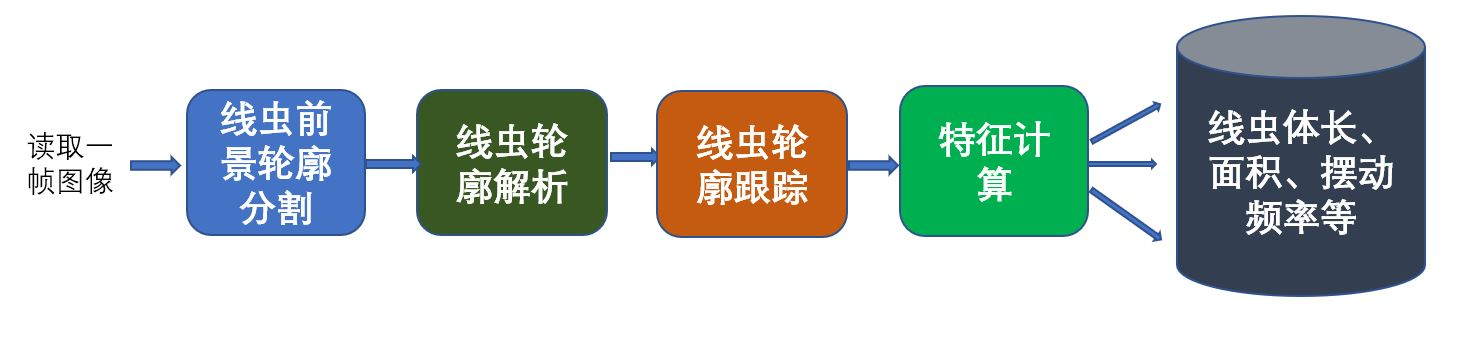
\includegraphics[width=14cm]{figure/chap3/flow.jpg}
	  % \hspace{1cm}
	  % 
\includegraphics[width=4cm]{example/sjtulogo.jpg}
	  \bicaption[这里将出现在插图索引中]
		{线虫图像处理总体流程图}
		{The flow chart of C.elegans image processing}
	  \label{fig:flow}
	\end{figure}
\section{基于背景减除方法的线虫轮廓分割}
	通过背景减除方法实现前景轮廓提取需要对背景进行建模,假设在一幅图像中每个像素的取值具有空间独立性
	,只与最近的T个历史像素取值相关。在时间$t$历史像素可以表示为$h_T=\{x^{(t)},\dots,x^{(t-T)}\}$,
	则每个像素的取值用一个包含M个高斯的混合高斯概率函数来建模,公式\ref{eq:gmm}中$FG$表示像素属于前景,$BG$表示
	该像素属于背景。$\hat{u}_1,\dots,\hat{u}_M$和$\hat{\sigma}_1^2,\dots,\hat{\sigma}_M^2$分别表示混合高斯模型中的待估参数均值和方差。
	$\hat{\pi}_m$表示高斯权重且所有权重相加等于1。
	\begin{equation}
		p(\vec{x}|h_T,BG+FG)= \sum_{m=1}^{M} \hat{\pi}_{m}N(\vec{x};\hat{u}_m,\hat{\sigma}_m^2I)\label{eq:gmm}
	\end{equation}
	当在时刻t得到一个新像素值$\vec{x}^{(t)}$时,模型参数将如下方式更新,其中$\vec{\delta}_m=\vec{x}^{(t)}-\hat{u}_m$,
	$a=1/T$。并将与新像素值$\vec{x}^{(t)}$最近的高斯分量对应的$o_m^{(t)}$设置为1其他设置为0。
	\begin{equation}
		\hat{\pi}_m \leftarrow \hat{\pi}_m +a(o_m^{(t)}-\hat{\pi}_m) \label{eq:updata}
	\end{equation}
	\begin{equation}
		\hat{u}_m \leftarrow \hat{u}_m +o_m^{(t)}(a/\hat{\pi}_m)\vec{\delta}_m \label{eq:updata1}
	\end{equation}
	\begin{equation}
		\hat{\sigma}_m^2 \leftarrow \hat{\sigma}_m^2 +o_m^{(t)}(a/\hat{\pi}_m)(\vec{\delta}_m^T\vec{\delta}_m-\hat{\sigma}_m^2) \label{eq:updata2}
	\end{equation}
	将M个高斯分量按照权重从大到小排序,则背景模型可以通过前B个最大的高斯分量来近似。
	\begin{equation}
		p(\vec{x}|h_T,BG) \sim \sum_{m=1}^{B} \hat{\pi}_{m}N(\vec{x};\hat{u}_m,\hat{\sigma}_m^2I)\label{eq:bg}
	\end{equation}
	如图\ref{fig:bgsub}所示基于混合高斯
	模型的背景减除方法与简单的帧间差分法相比,背景减除的方法能够显著的减少前景轮廓提取的不连续分割的性能
	更好。用一个$5\times5$的核对提取到的前景轮廓进行形态学闭运算得到的结果如图\ref{fig:bgsub:close}所示。
	最后,运用OTSU二值化算法就可以得到最终的线虫前景轮廓如图\ref{fig:bgsub:bin}所示。

	
% \begin{figure*}
% \centering
% \subfigure[Input]{
% \begin{minipage}[b]{0.23\linewidth}
% 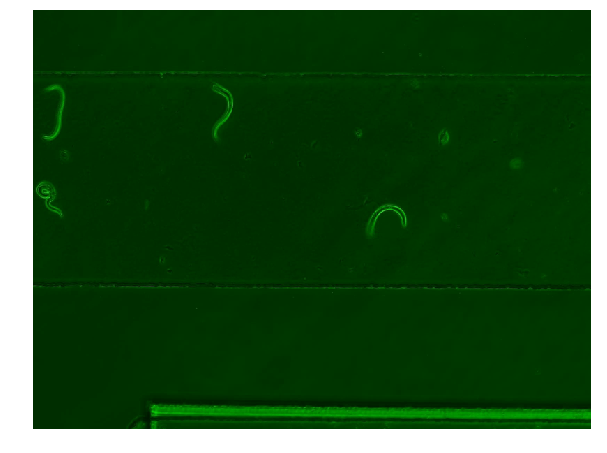
\includegraphics[width=1\linewidth]{figure/chap3/worm.png}\vspace{4pt}
% 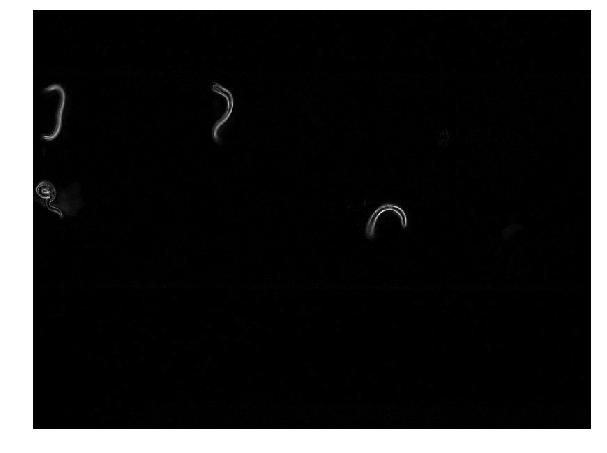
\includegraphics[width=1\linewidth]{figure/chap3/bgsub.png}\vspace{4pt}
% 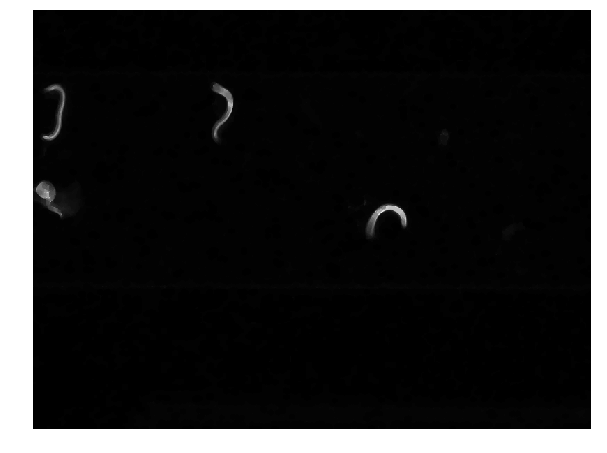
\includegraphics[width=1\linewidth]{figure/chap3/close.png}
% \end{minipage}}
% \subfigure[CE]{
% \begin{minipage}[b]{0.23\linewidth}
% 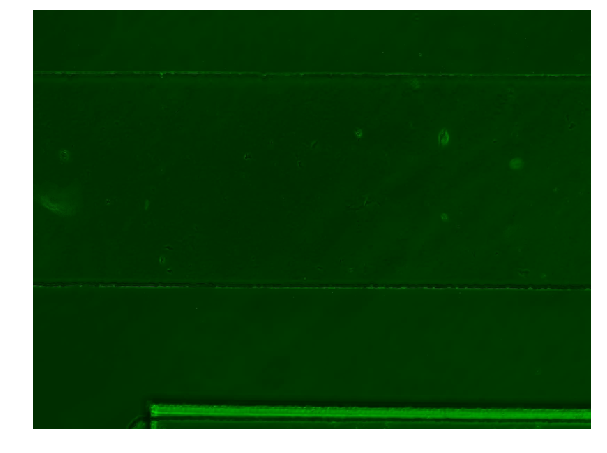
\includegraphics[width=1\linewidth]{figure/chap3/bg.png}\vspace{4pt}
% 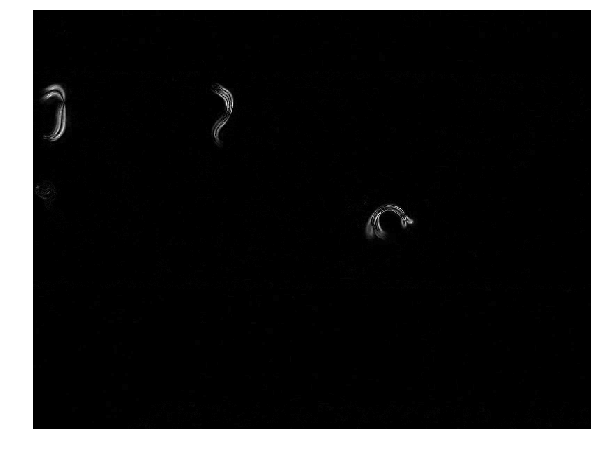
\includegraphics[width=1\linewidth]{figure/chap3/difffra.png}\vspace{4pt}
% 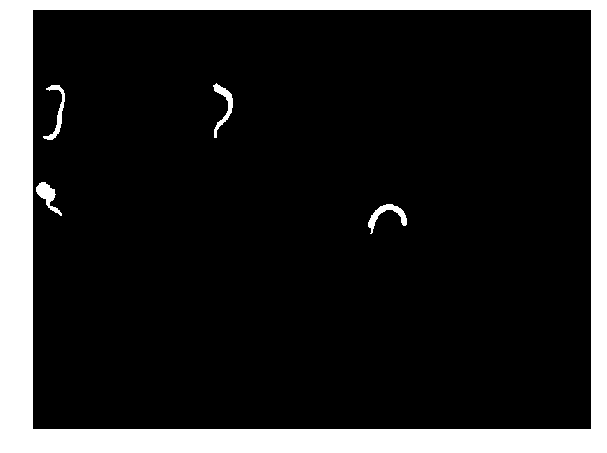
\includegraphics[width=1\linewidth]{figure/chap3/otsu.png}
% \end{minipage}}
% \caption{description of figure}
% \end{figure*}
\begin{figure}[h]
  \centering
  \begin{subfigure}{0.4\textwidth}
    \centering
    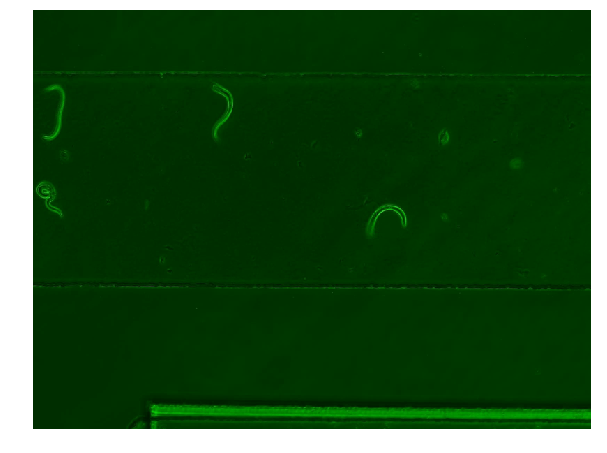
\includegraphics[width=1\linewidth]{figure/chap3/worm.png}
    \caption{待处理线虫图像}
	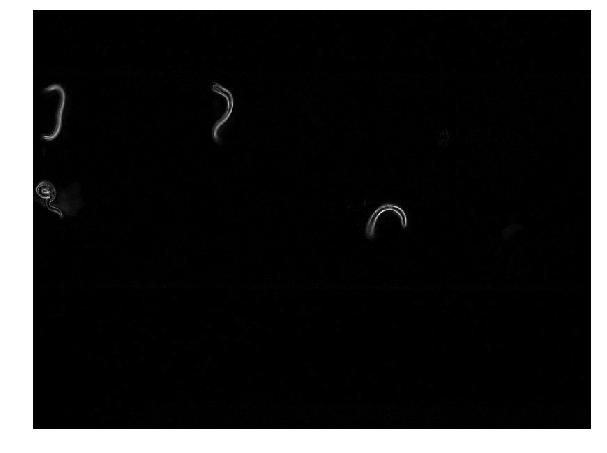
\includegraphics[width=1\linewidth]{figure/chap3/bgsub.png}
	\caption{基于混合高斯模型背景减除图片}
	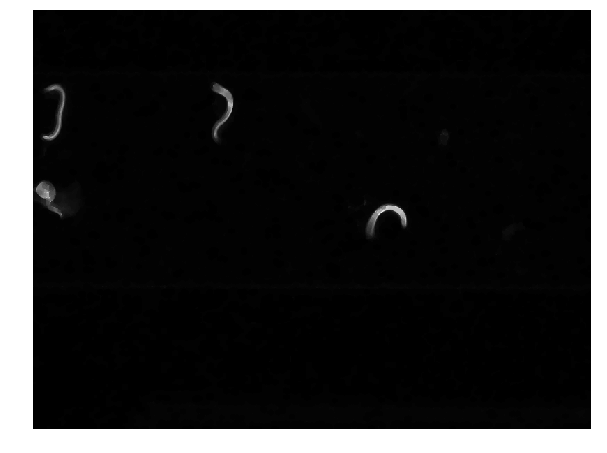
\includegraphics[width=1\linewidth]{figure/chap3/close.png}
	\caption{对背景减除得到的图像闭运算}\label{fig:bgsub:close}
  \end{subfigure}
  \hspace{4em}
  \begin{subfigure}{0.4\textwidth}
    \centering
    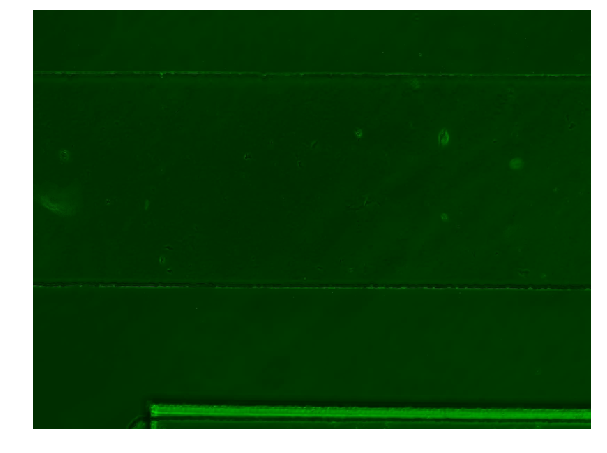
\includegraphics[width=1\linewidth]{figure/chap3/bg.png}
    \caption{基于混合高斯模型建模的背景图}
	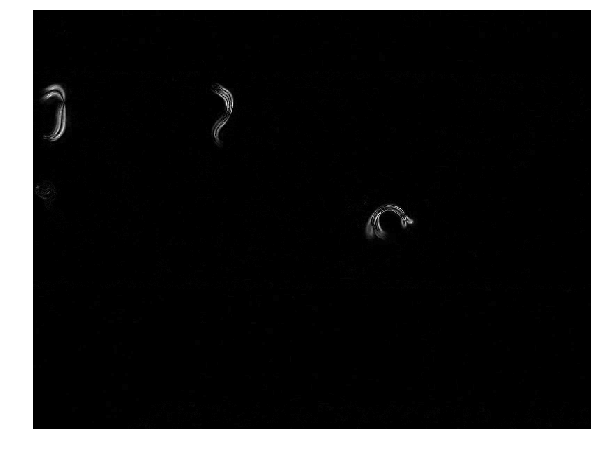
\includegraphics[width=1\linewidth]{figure/chap3/difffra.png}
	\caption{帧间差分法结果图}
	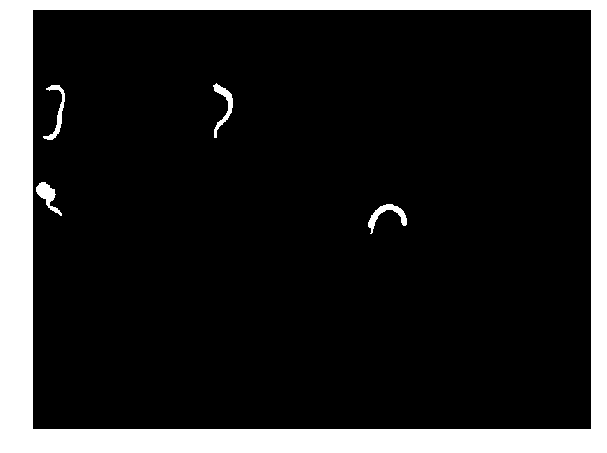
\includegraphics[width=1\linewidth]{figure/chap3/otsu.png}
	\caption{OTSU阈值处理后的二值图}\label{fig:bgsub:bin}
  \end{subfigure}
  \bicaption{前景提取过程中的图片}{The images in the foreground object extraction}
  \label{fig:bgsub}
\end{figure}
\section{线虫轮廓的跟踪}
	由于线虫通体透明,跟踪起来比较困难,本文采用了一种简单有效的跟踪策略。首先经过
	线虫前景轮廓提取和线虫轮廓解析等步骤后,可以得到每一帧图像里所有线虫的轮廓。由
	公式\ref{eq:m}和公式\ref{eq:xy}可以计算出轮廓的重心坐标。
	\begin{equation}
		m_{ji}=\sum_{x,y}I_{x,y}x^iy^j \label{eq:m}
	\end{equation}
	\begin{equation}
		\vec{x}=\frac{m_{10}}{m_{00}},\quad \vec{y}=\frac{m_{01}}{m_{00}}\label{eq:xy}
	\end{equation}
	假设当前帧有n个轮廓,上一帧
	图像有m个轮廓,由每个轮廓的重心坐标可以得到一个$n\times m$的距离矩阵用公式\ref{eq:matrix}
	表示。
		\begin{equation}
                        D=\left[
                \begin{matrix}
                 d_{11}      & d_{12}      & \cdots & d_{1m}      \\
                 d_{21}      & d_{22}      & \cdots & d_{2m}      \\
                 \vdots & \vdots & \ddots & \vdots \\
                 d_{n1}      & d_{n2}      & \cdots & d_{nm}      \\
                \end{matrix}
                \right]\label{eq:matrix}
    \end{equation}
	矩阵中$d_{ij}$表示当前帧中的第i个轮廓的重心到上一帧中第j个轮廓的重心之间的距离。通过
	公式\ref{eq:min}可以得到相邻两帧图像中线虫轮廓之间的对应关系。即如果相邻两帧图像中两个
	轮廓重心之间的距离最短,则可以认为是同一个线虫。
		\begin{equation}
        index(i)=\mathop{\arg\min}_{j} d_{ij}\label{eq:min}
		\end{equation}
	但事实上由于轮廓分割的不完美以及图像噪声的影响
	,这一策略往往会失效。因此,通过最近邻搜索的方式来实现线虫的跟踪要满足以下的约束条件,当这两个
	条件之一不满足时,则认为跟踪丢失,此时应该分配一个新的trackID给当前的轮廓。算法\ref{algo:worm_track}
	是描述了线虫跟踪算法的实现思路。
	
	\begin{itemize}
	  \item 相邻两帧图像中同一只线虫的轮廓面积的相对变化应该小于一个阈值。
	  \item 根据线虫运动的最大速度,同一只线虫在相邻两帧图像中轮廓的重心之间的距离应该小于一个阈值。
	\end{itemize}

\begin{algorithm}
\caption{跟踪初始化程序}
\label{algo:initial_track}
\begin{algorithmic}[1]
	\Require $Worm\_data$双重列表,$Worm\_data[i][j]$表示第$i$帧图像中第$j$只线虫。
	\Ensure 输出$trackID$
	\Function {Initiate\_tracking}{$Worm\_data$}
		\State $FirstFrame\_WormData \gets Worm\_data[0]$
		\For{$i = 0 \to FirstFrame\_WormData.length-1$}
			\State $cur\_worm \gets FirstFrame\_WormData[i]$
			\State $cur\_worm.trackID \gets GetNewTrackID()$
		\EndFor
\EndFunction
\end{algorithmic}
\end{algorithm}

\begin{algorithm}[H]
\caption{线虫跟踪程序}
\label{algo:worm_track}
\begin{algorithmic}[1]
	\Require $Worm\_data$双重列表,$Worm\_data[i][j]$表示第$i$帧图像中第$j$只线虫。
	\Ensure 输出$trackID$
	\Function {Worm\_tracking}{$Worm\_data$}
		\State $Initiate\_tracking(Worm\_data)$
		\For{$frame_index = 1 \to Worm\_Data.length-1$}
			\State $PreFrame\_WormData \gets Worm\_Data[frame_index-1] $
			\For{$worm\_index =0 \to Worm\_Data[frame_index].length-1$}
\algstore{WormTracking}
\end{algorithmic}
\end{algorithm}
\begin{algorithm}[H]
\begin{algorithmic}[1]
\algrestore{WormTracking}
		
				\State $cur\_worm \gets Worm\_Data[frame\_index][worm\_index]$
				\State $dist\_array \gets Compute\_distance(cur\_worm,PreFrame\_WormData)$
				\State $min\_index \gets Get\_min\_index(dist\_array)$
				\State $Nearest\_worm \gets PreFrame\_WormData[min\_index]$
				\If{$\small{\frac{|Nearest\_worm.Area-cur\_worm.Area|}{Nearest\_worm.Area}<\delta \quad \text{and}  \quad dist\_array[min\_index]< \sigma}$}
					\State $cur\_worm.trackID \gets Nearest\_worm.trackID$
				\Else
					\State $cur\_worm.trackID \gets GetNewTrackID( )$
				\EndIf
			\EndFor
		\EndFor
\EndFunction
\end{algorithmic}
\end{algorithm}
\section{线虫的特征提取}
\subsection{线虫轮廓中间脊线提取}


\section{本章小结}



\chapter{基于深度卷积网络的线虫轮廓解析}

\section{线虫轮廓解析方法介绍}

\section{Singleout 网络设计及模型评估}


\section{论文研究的背景及意义}

\section{论文研究的背景及意义}
\chapter{线虫的特征提取和急性氧化应激实验}
\section{引言}
	在前面的章节中,本文已经介绍了线性梯度稀释芯片的设计以及线虫前景轮廓的分割与单线虫轮廓的解析。
	本章我们将首先介绍线虫轮廓的跟踪,然后介绍基于线虫轮廓跟踪的结果计算线虫的摆动频率特征。最后,通过运用
	本文提出的软硬件系统研究不同线性浓度双氧水对线虫摆动频率的影响,从而验证了本文提出的软硬件平台在高通量自动化药物筛选
	方面具有一定的优势。
\section{线虫轮廓的跟踪}
	由于线虫通体透明,跟踪起来比较困难,本文采用了一种简单有效的跟踪策略。首先经过
	线虫前景轮廓提取和线虫轮廓解析等步骤后,可以得到每一帧图像里所有线虫的轮廓。由
	公式\ref{eq:m}和公式\ref{eq:xy}可以计算出轮廓的重心坐标。
	\begin{equation}
		m_{ji}=\sum_{x,y}I_{x,y}x^iy^j \label{eq:m}
	\end{equation}
	\begin{equation}
		\vec{x}=\frac{m_{10}}{m_{00}},\quad \vec{y}=\frac{m_{01}}{m_{00}}\label{eq:xy}
	\end{equation}
	假设当前帧有n个轮廓,上一帧
	图像有m个轮廓,由每个轮廓的重心坐标可以得到一个$n\times m$的距离矩阵用公式\ref{eq:matrix}
	表示。
		\begin{equation}
                        D=\left[
                \begin{matrix}
                 d_{11}      & d_{12}      & \cdots & d_{1m}      \\
                 d_{21}      & d_{22}      & \cdots & d_{2m}      \\
                 \vdots & \vdots & \ddots & \vdots \\
                 d_{n1}      & d_{n2}      & \cdots & d_{nm}      \\
                \end{matrix}
                \right]\label{eq:matrix}
    \end{equation}
	\begin{figure}[t]
	  \centering
	  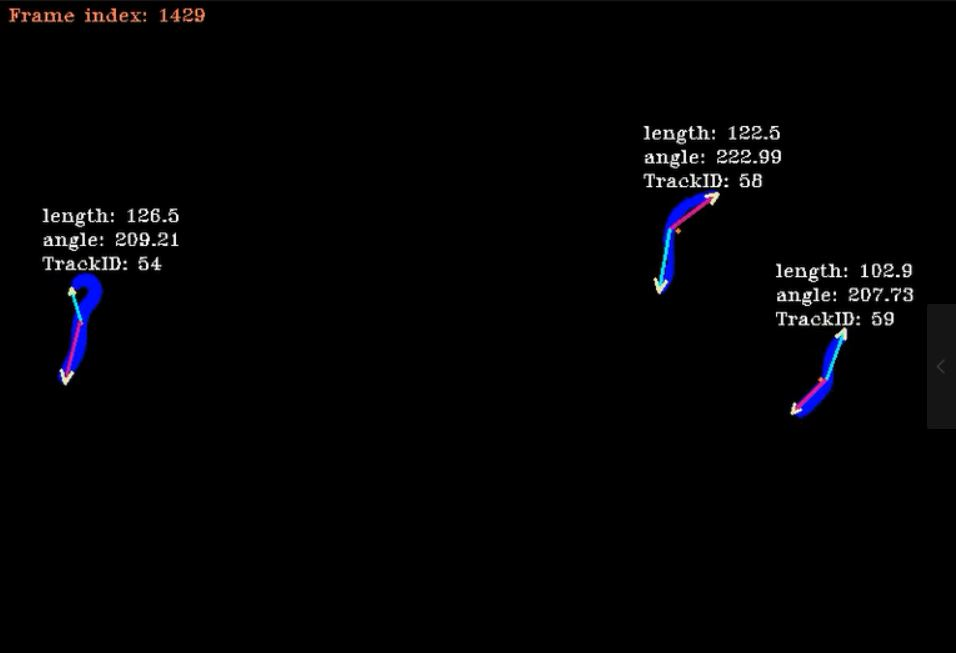
\includegraphics[width=9cm]{figure/chap5/tracking.jpg}
	  \bicaption[这里将出现在插图索引中]
		{跟踪的结果}
		{The tracking result}
	  \label{fig:track}
	\end{figure}
	矩阵中$d_{ij}$表示当前帧中的第i个轮廓的重心到上一帧中第j个轮廓的重心之间的距离。通过
	公式\ref{eq:min}可以得到相邻两帧图像中线虫轮廓之间的对应关系。即如果相邻两帧图像中两个
	轮廓重心之间的距离最短,则可以认为是同一个线虫。
		\begin{equation}
        index(i)=\mathop{\arg\min}_{j} d_{ij}\label{eq:min}
		\end{equation}
	但事实上由于轮廓分割的不完美以及图像噪声的影响
	,这一策略往往会失效。因此,通过最近邻搜索的方式来实现线虫的跟踪要满足以下的约束条件,当这两个
	条件之一不满足时,则认为跟踪丢失,此时应该分配一个新的trackID给当前的轮廓。算法\ref{algo:worm_track}
	是描述了线虫跟踪算法的实现思路。图\ref{fig:track}表示跟踪的结果。
	
	\begin{itemize}
	  \item 相邻两帧图像中同一只线虫的轮廓面积的相对变化应该小于一个阈值。
	  \item 根据线虫运动的最大速度,同一只线虫在相邻两帧图像中轮廓的重心之间的距离应该小于一个阈值。
	\end{itemize}

\begin{algorithm}
\caption{跟踪初始化程序}
\label{algo:initial_track}
\begin{algorithmic}[1]
	\Require $Worm\_data$双重列表,$Worm\_data[i][j]$表示第$i$帧图像中第$j$只线虫。
	\Ensure 输出$trackID$
	\Function {Initiate\_tracking}{$Worm\_data$}
		\State $FirstFrame\_WormData \gets Worm\_data[0]$
		\For{$i = 0 \to FirstFrame\_WormData.length-1$}
			\State $cur\_worm \gets FirstFrame\_WormData[i]$
			\State $cur\_worm.trackID \gets GetNewTrackID()$
		\EndFor
\EndFunction
\end{algorithmic}
\end{algorithm}

\begin{algorithm}[H]
\caption{线虫跟踪程序}
\label{algo:worm_track}
\begin{algorithmic}[1]
	\Require $Worm\_data$双重列表,$Worm\_data[i][j]$表示第$i$帧图像中第$j$只线虫。
	\Ensure 输出$trackID$
	\Function {Worm\_tracking}{$Worm\_data$}
		\State $Initiate\_tracking(Worm\_data)$
		\For{$frame_index = 1 \to Worm\_Data.length-1$}
			\State $PreFrame\_WormData \gets Worm\_Data[frame_index-1] $
			\For{$worm\_index =0 \to Worm\_Data[frame_index].length-1$}
% \algstore{WormTracking}
% \end{algorithmic}
% \end{algorithm}
% \begin{algorithm}[H]
% \begin{algorithmic}[1]
% \algrestore{WormTracking}
		
				\State $cur\_worm \gets Worm\_Data[frame\_index][worm\_index]$
				\State $dist\_array \gets Compute\_distance(cur\_worm,PreFrame\_WormData)$
				\State $min\_index \gets Get\_min\_index(dist\_array)$
				\State $Nearest\_worm \gets PreFrame\_WormData[min\_index]$
				\If{$\small{\frac{|Nearest\_worm.Area-cur\_worm.Area|}{Nearest\_worm.Area}<\delta \quad \text{and}  \quad dist\_array[min\_index]< \sigma}$}
					\State $cur\_worm.trackID \gets Nearest\_worm.trackID$
				\Else
					\State $cur\_worm.trackID \gets GetNewTrackID( )$
				\EndIf
			\EndFor
		\EndFor
\EndFunction
\end{algorithmic}
\end{algorithm}
\section{线虫的特征提取}
	线虫从头部到尾部两边近似等距的分布着23-24块肌肉,其头部和尾部各占其总长度的$1/6$。因此线虫
	身体的自由度为24。当用轮廓来描述线虫的形态时,在其轮廓上采样49个点足以描述线虫所有形态。
	当对线虫进行特征计算时(如:计算线虫摆动频率和运动速度等),通常是利用线虫轮廓中间的脊线进行计算。
	因此需要提取线虫轮廓的中线然后采样24个点用于特征计算。下面将首先对线虫轮廓中间脊线提取算法进行介绍,
	然后介绍线虫摆动频率的估计以及运动速度的计算。
\subsection{线虫轮廓中间脊线提取}
	在得到线虫的轮廓后,将轮廓上的坐标按顺时针排列即可得到一个坐标点的循环列表。将轮廓周长的$1/48$作为一个单位边,
	在轮廓上的任意一点其两边都可以找到一个单位边长度的相邻点,这三点所成角的补角的倒数与该点的曲率成正比,因此
	可以用于近似曲率的计算。由于其头部和尾部的变换往往比身体的其他部分要尖锐,所以如果将像素索引作为横坐标曲率作为
	纵坐标,则这条曲线上将会出现两个波峰如图\ref{fig:qulv}所示,分别对应线虫的头部和尾部。由此便可定位到线虫的头部和尾部,另外线虫的头部
	曲率一般小于尾部的曲率,两个波峰中比较低的波峰对应的横坐标为线虫头部的坐标,另一个波峰对应线虫尾部的坐标。
	线虫头部和尾部将线虫轮廓分为两边。在其中一条边上找到所有距离另一条边最近的对应点。两条边上两对应点的中点构成线虫的
	中间脊线,线虫轮廓中间脊线的长度定义为线虫的体长。
	\begin{figure}[h]
	  \centering
	  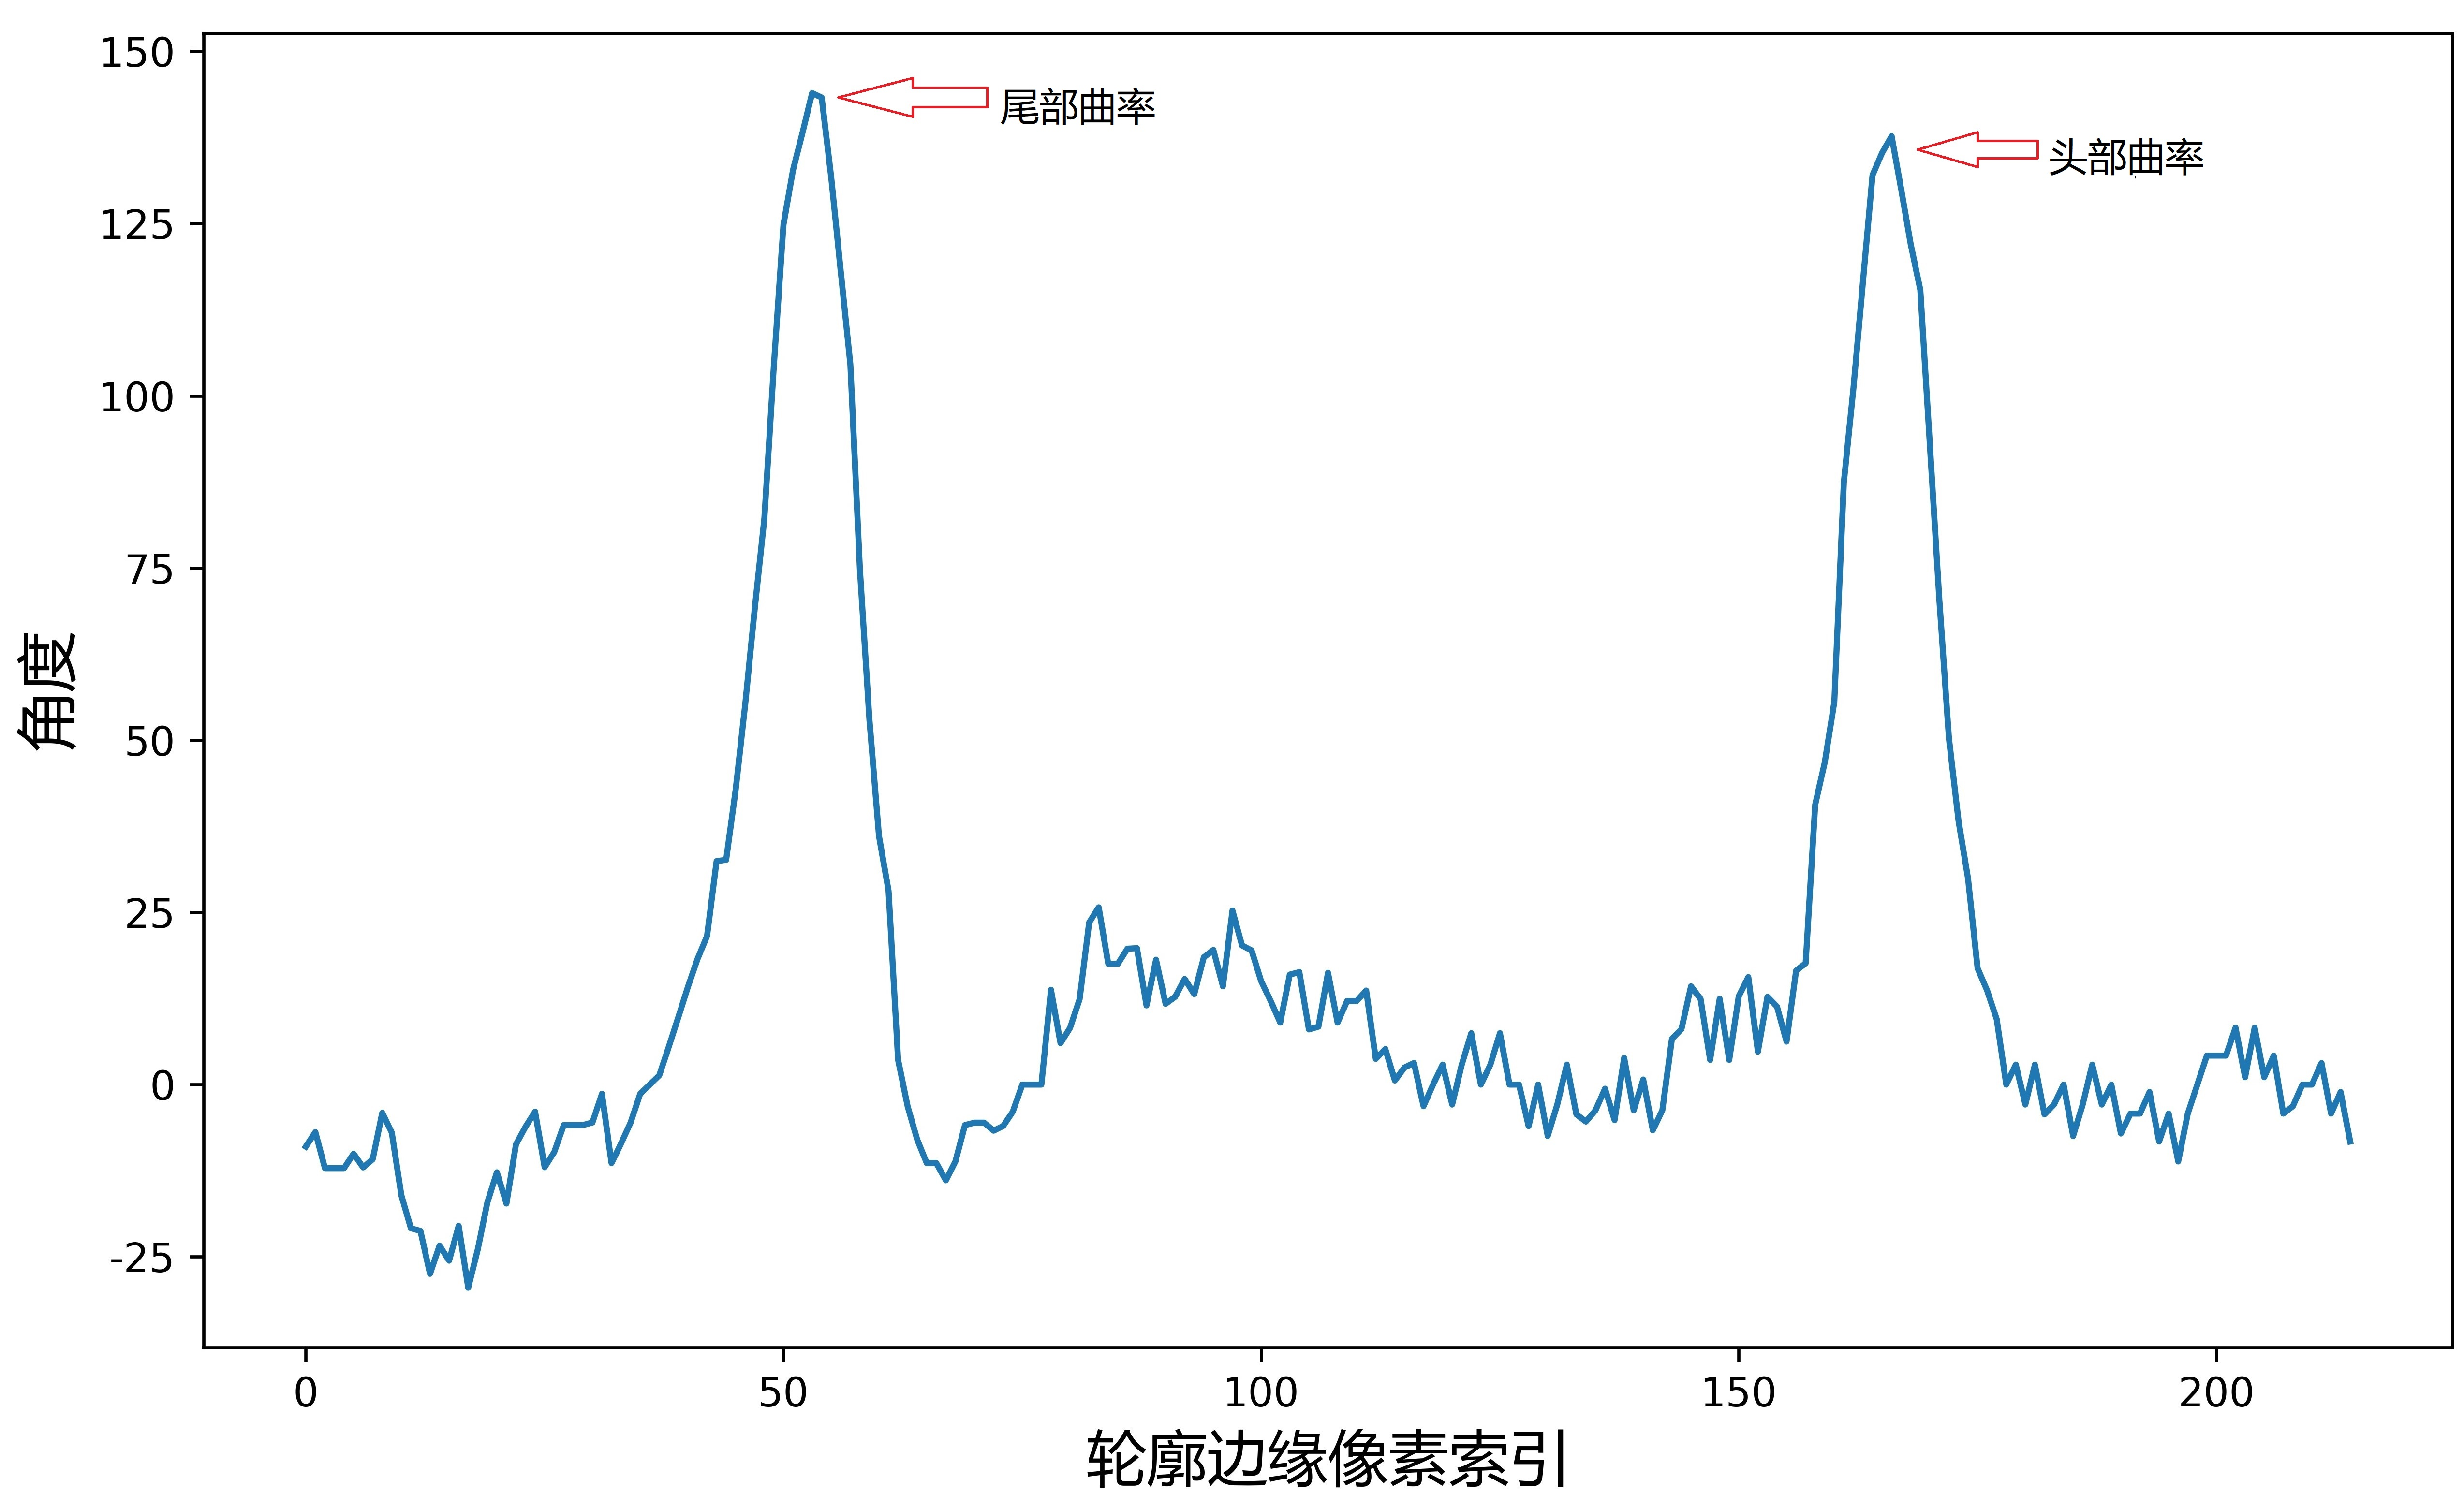
\includegraphics[width=14cm]{figure/chap5/cuvature.jpg}
	  \bicaption[这里将出现在插图索引中]
		{轮廓曲率的变化}
		{Change in contour curvature}
	  \label{fig:qulv}
	\end{figure}
\subsection{身体弯曲角度的计算以及摆动频率的估计}
	在很多毒理实验中,线虫的摆动频率经常作为一个重要的生理指标用于表征线虫的活跃程度\cite{Wang2008Assessment}。
	为了计算线虫的摆动频率, 我们定义一个衡量身体弯曲程度的夹角,由线虫头部、尾部和轮廓脊线的中点三点所成角定义为
	身体弯曲角如图\ref{fig:track}所示。线虫在爬行和游动的过程中,身体弯曲角会在$180^\circ$C左右振荡如图\ref{fig:angle},
	振荡的频率定义为线虫摆动的频率。在时刻$t_0$,对区间$(t_0-\Delta t,t_0+\Delta t)$中弯曲角信号做FFT变换,假设其幅度最大值对应的横坐标
	为n,则线虫在$t$时刻的瞬时摆动频率由公式\ref{eq:freq}得出,图\ref{fig:freq}表示线虫摆动频率随时间的变换。
	\begin{equation}
        f=\frac{frame\_rate*n}{2*\Delta t} \label{eq:freq}
	\end{equation}
		
\begin{figure}[!htp]    
% \begin{minipage}[t]{0.5\linewidth}%设定图片下字的宽度,在此基础尽量满足图片的长宽    
	\centering    
	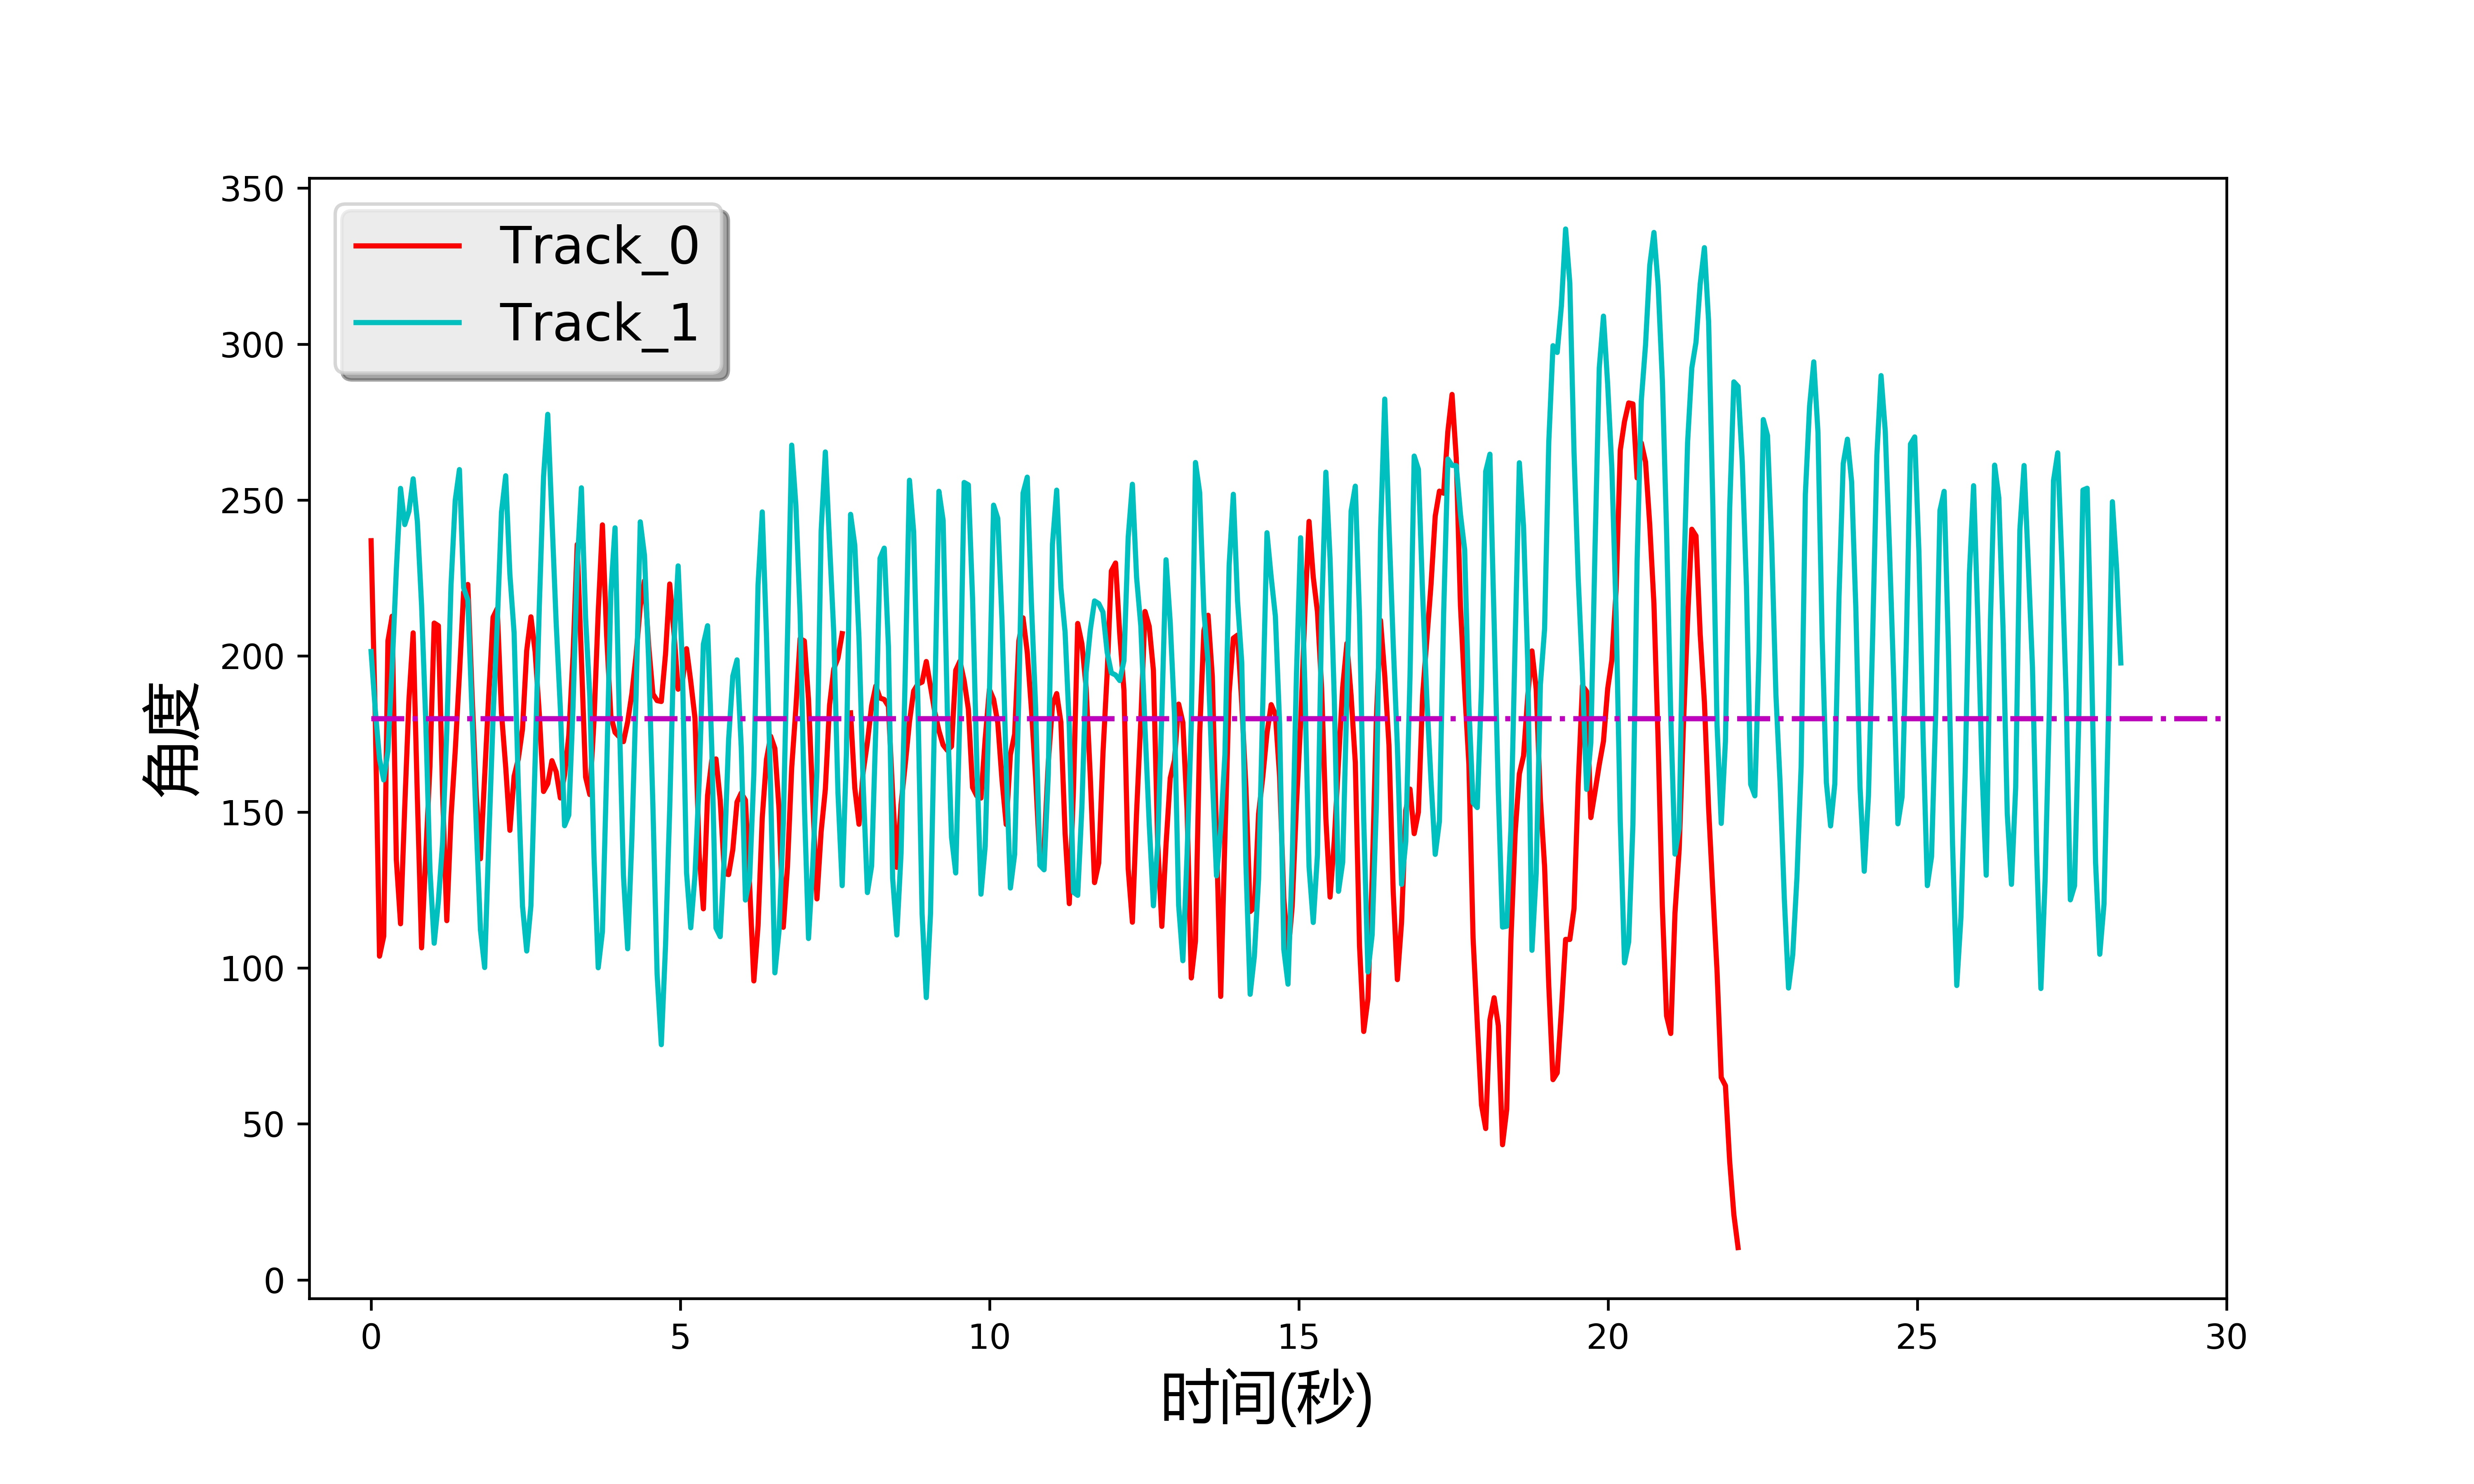
\includegraphics[width=1\linewidth]{figure/chap3/angle.jpg}    
	% \caption*{(a) 弯曲角的变化}%加*可以去掉默认前缀,作为图片单独的说明    
	% \label{fig:angle}    
% \end{minipage}    
% \begin{minipage}[t]{0.5\linewidth}%需要几张添加即可,注意设定合适的linewidth    
	% \centering    
	% 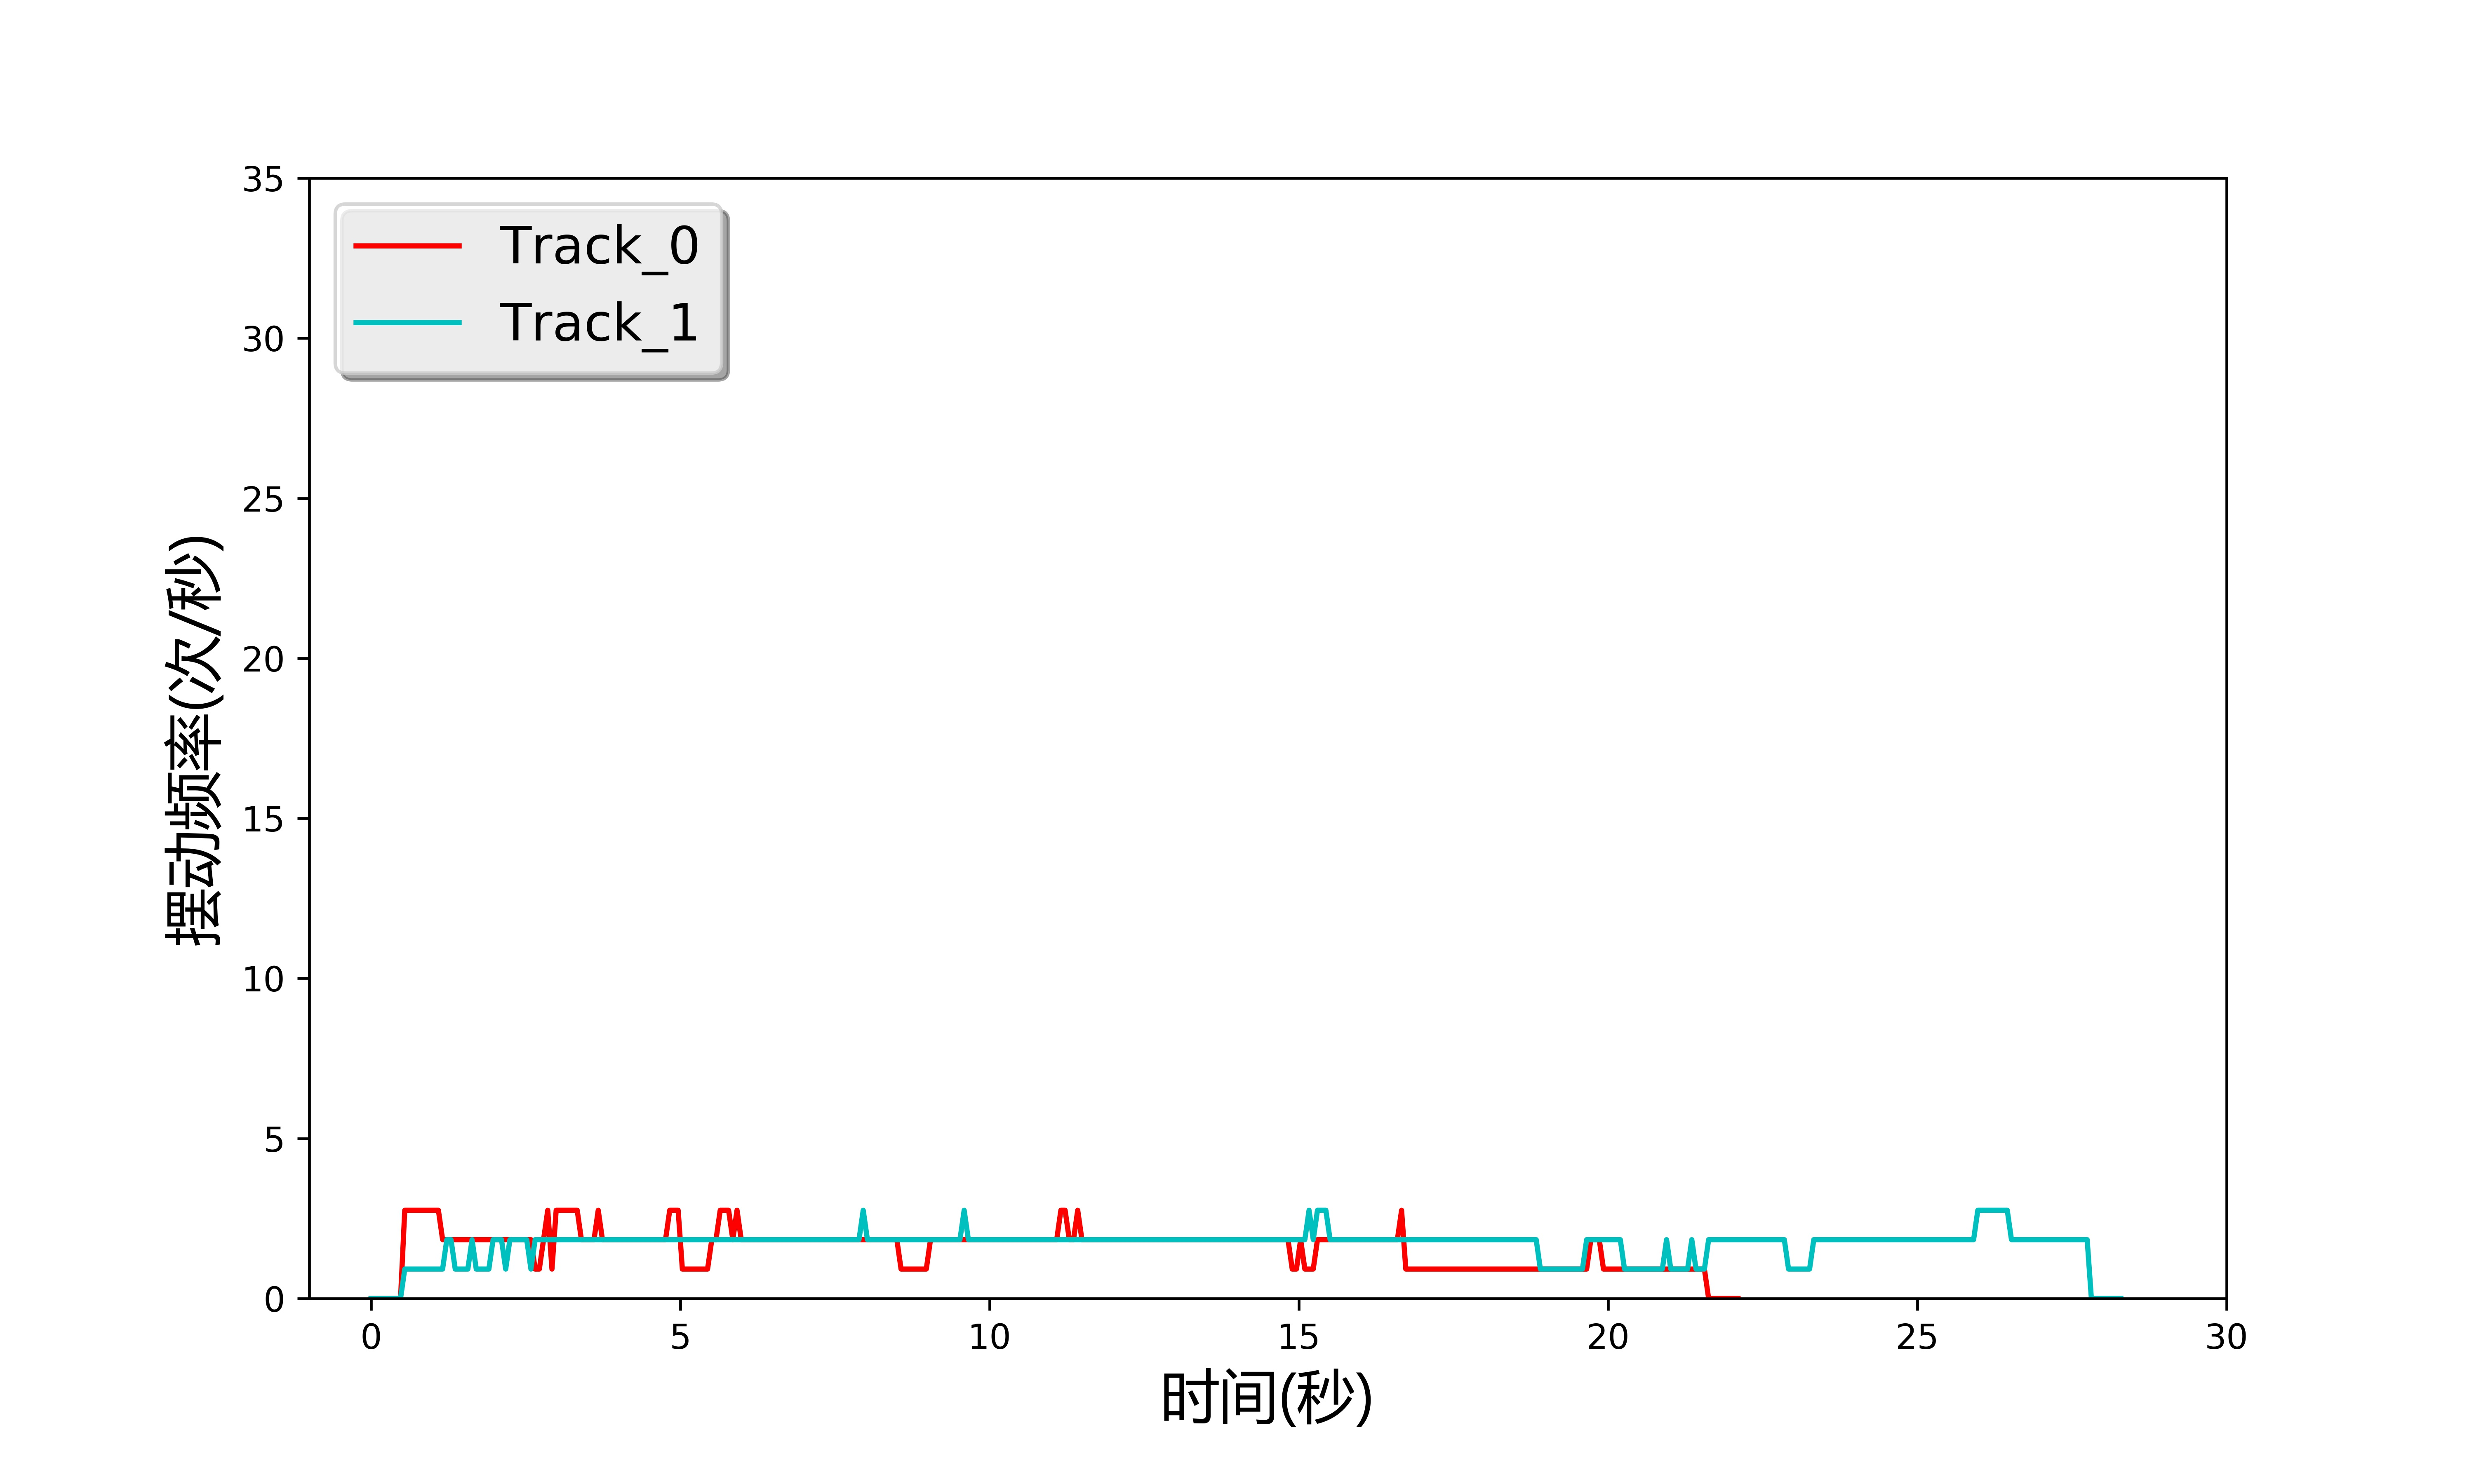
\includegraphics[width=1\linewidth]{figure/chap3/freq.jpg}    
	% \caption*{(b) 摆动频率的变化}
	% \label{fig:freq}
% \end{minipage}
\bicaption{线虫弯曲角度和摆动频率的变换}{An EPS and PDF demo with subcaptionbox}%n张图片共享的说明
\end{figure}
\section{线虫的氧化急性应激实验}
	氧化应激(Oxidative Stress,OS)指生物体氧化与抗氧化作用的失衡,当生物体被内外环境中
	存在有害化合物刺激时,其体内所产生的活性氮自由基和活性氧自由基将会导致细胞或者组织发生生理和
	病理反应。过氧化氢($H_2O_2$)溶液作为一种强氧化剂经常被用于线虫的氧化应激实验中。本文
	将野生型N2秀丽隐杆线虫的L1期幼虫作为研究对象,通过本文前面介绍的软硬件平台,研究不同线性
	浓度梯度的双氧水溶液对L1期幼虫活性的影响。
\subsection{线虫的同步化}
	为了得到处于同一发育阶段的幼虫需要对线虫进行同步化处理,首先用经过高压灭菌的M9缓冲液将NGM平板上
	混合发育期的线虫冲洗到1.5ml的离心管中,离心后去掉上清液,加入碱裂解液(体积比为1:2的5N NaOH溶液和
	5\%NaClO溶液,现配),当线虫全被腐蚀时,液体将变得清澈。再经过离心处理,去掉上层碱裂解液加入M9
	缓冲液,离心洗涤1到2次。去掉上层缓冲液并用吸管将线虫卵接种到NGM平板上,至此便完成了同步化操作,等
	线虫卵孵化便得到同步化的个体。
\subsection{线性梯度稀释芯片的操作}
	图\ref{fig:sysdevice}是实验硬件部分连接示意图,芯片上所有的阀门控制和进样控制均由Arduino单片机
	通过uln2803集成芯片控制多路电磁阀实现。将含有L1期线虫的溶液离心去上清得到线虫浓缩液,
	然后用移液枪加入0.25\%的琼脂糖溶液作为线虫助悬剂。打开6号阀门,
	采用压力进样的方式将线虫溶液从4号进样口打入第三列腔室。
	打开4号阀门用压力进样的方式将水从3号进样口打入第二列腔室。
	然后打开2号阀门用压力进样的方式将30mM的过氧化氢溶液从2号进样口打入第一列腔室。
	然后关闭2号、4号和6号阀门,打开1号、3号、5号和7号阀门,
	并在一号进样口施加一个周期性的气压。通过振荡的方式使前三列腔室中的液体充分混合。
	最后通过进样口1将混合好的液体打入第四列腔室,根据芯片腔室的尺寸设计,可以计算出混合后各腔室的过氧化氢溶液的浓度从上至小依次为:
	18mM、16mM、14mM、12mM、10mM、8mM、6mM、4mM、2mM。并用CCD相机每隔10分钟采集线虫在9个腔室中的运动视频。
	\begin{figure}[h]
	  \centering
	  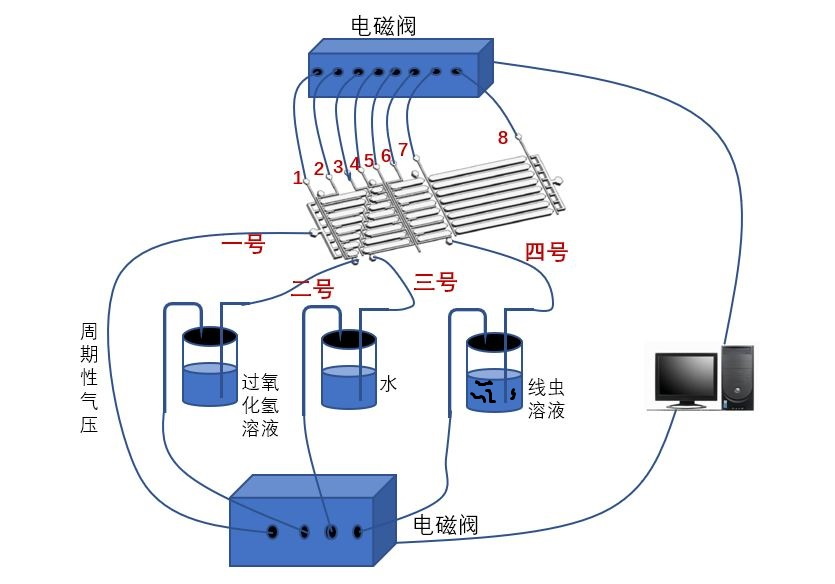
\includegraphics[width=12cm]{figure/chap5/hardware.jpg}
	  \bicaption[这里将出现在插图索引中]
		{实验系统装置示意图}
		{Change in contour curvature}
	  \label{fig:sysdevice}
	\end{figure}
\subsection{秀丽隐杆线虫急性氧化应激实验结果}
	通过本文提出的线虫轮廓分割、解析、跟踪及特征提取算法对每个腔室的各个时刻的视频进行分析并提取摆动频率特征,
	图\ref{fig:res}为了各腔室中线虫的平均摆动频率随时间的变化,可以看出随着过氧化氢溶液浓度的升高,线虫的摆动频率下降,
	且在同一浓度下,线虫的摆动频率随着时间而下降。为验证芯片实验的准确性,我们也在96孔板上手动稀释形成上述浓度后,
	通过对各个时间点线虫平均摆动频率的统计,实验结果表明96孔板实验和微流控芯片结果一致。但是相比96孔板实验,
	我们的微流控芯片平台在试剂消耗、自动分析等上面都体现了较大的优势。
	
	\begin{figure}[h]
	  \centering
	  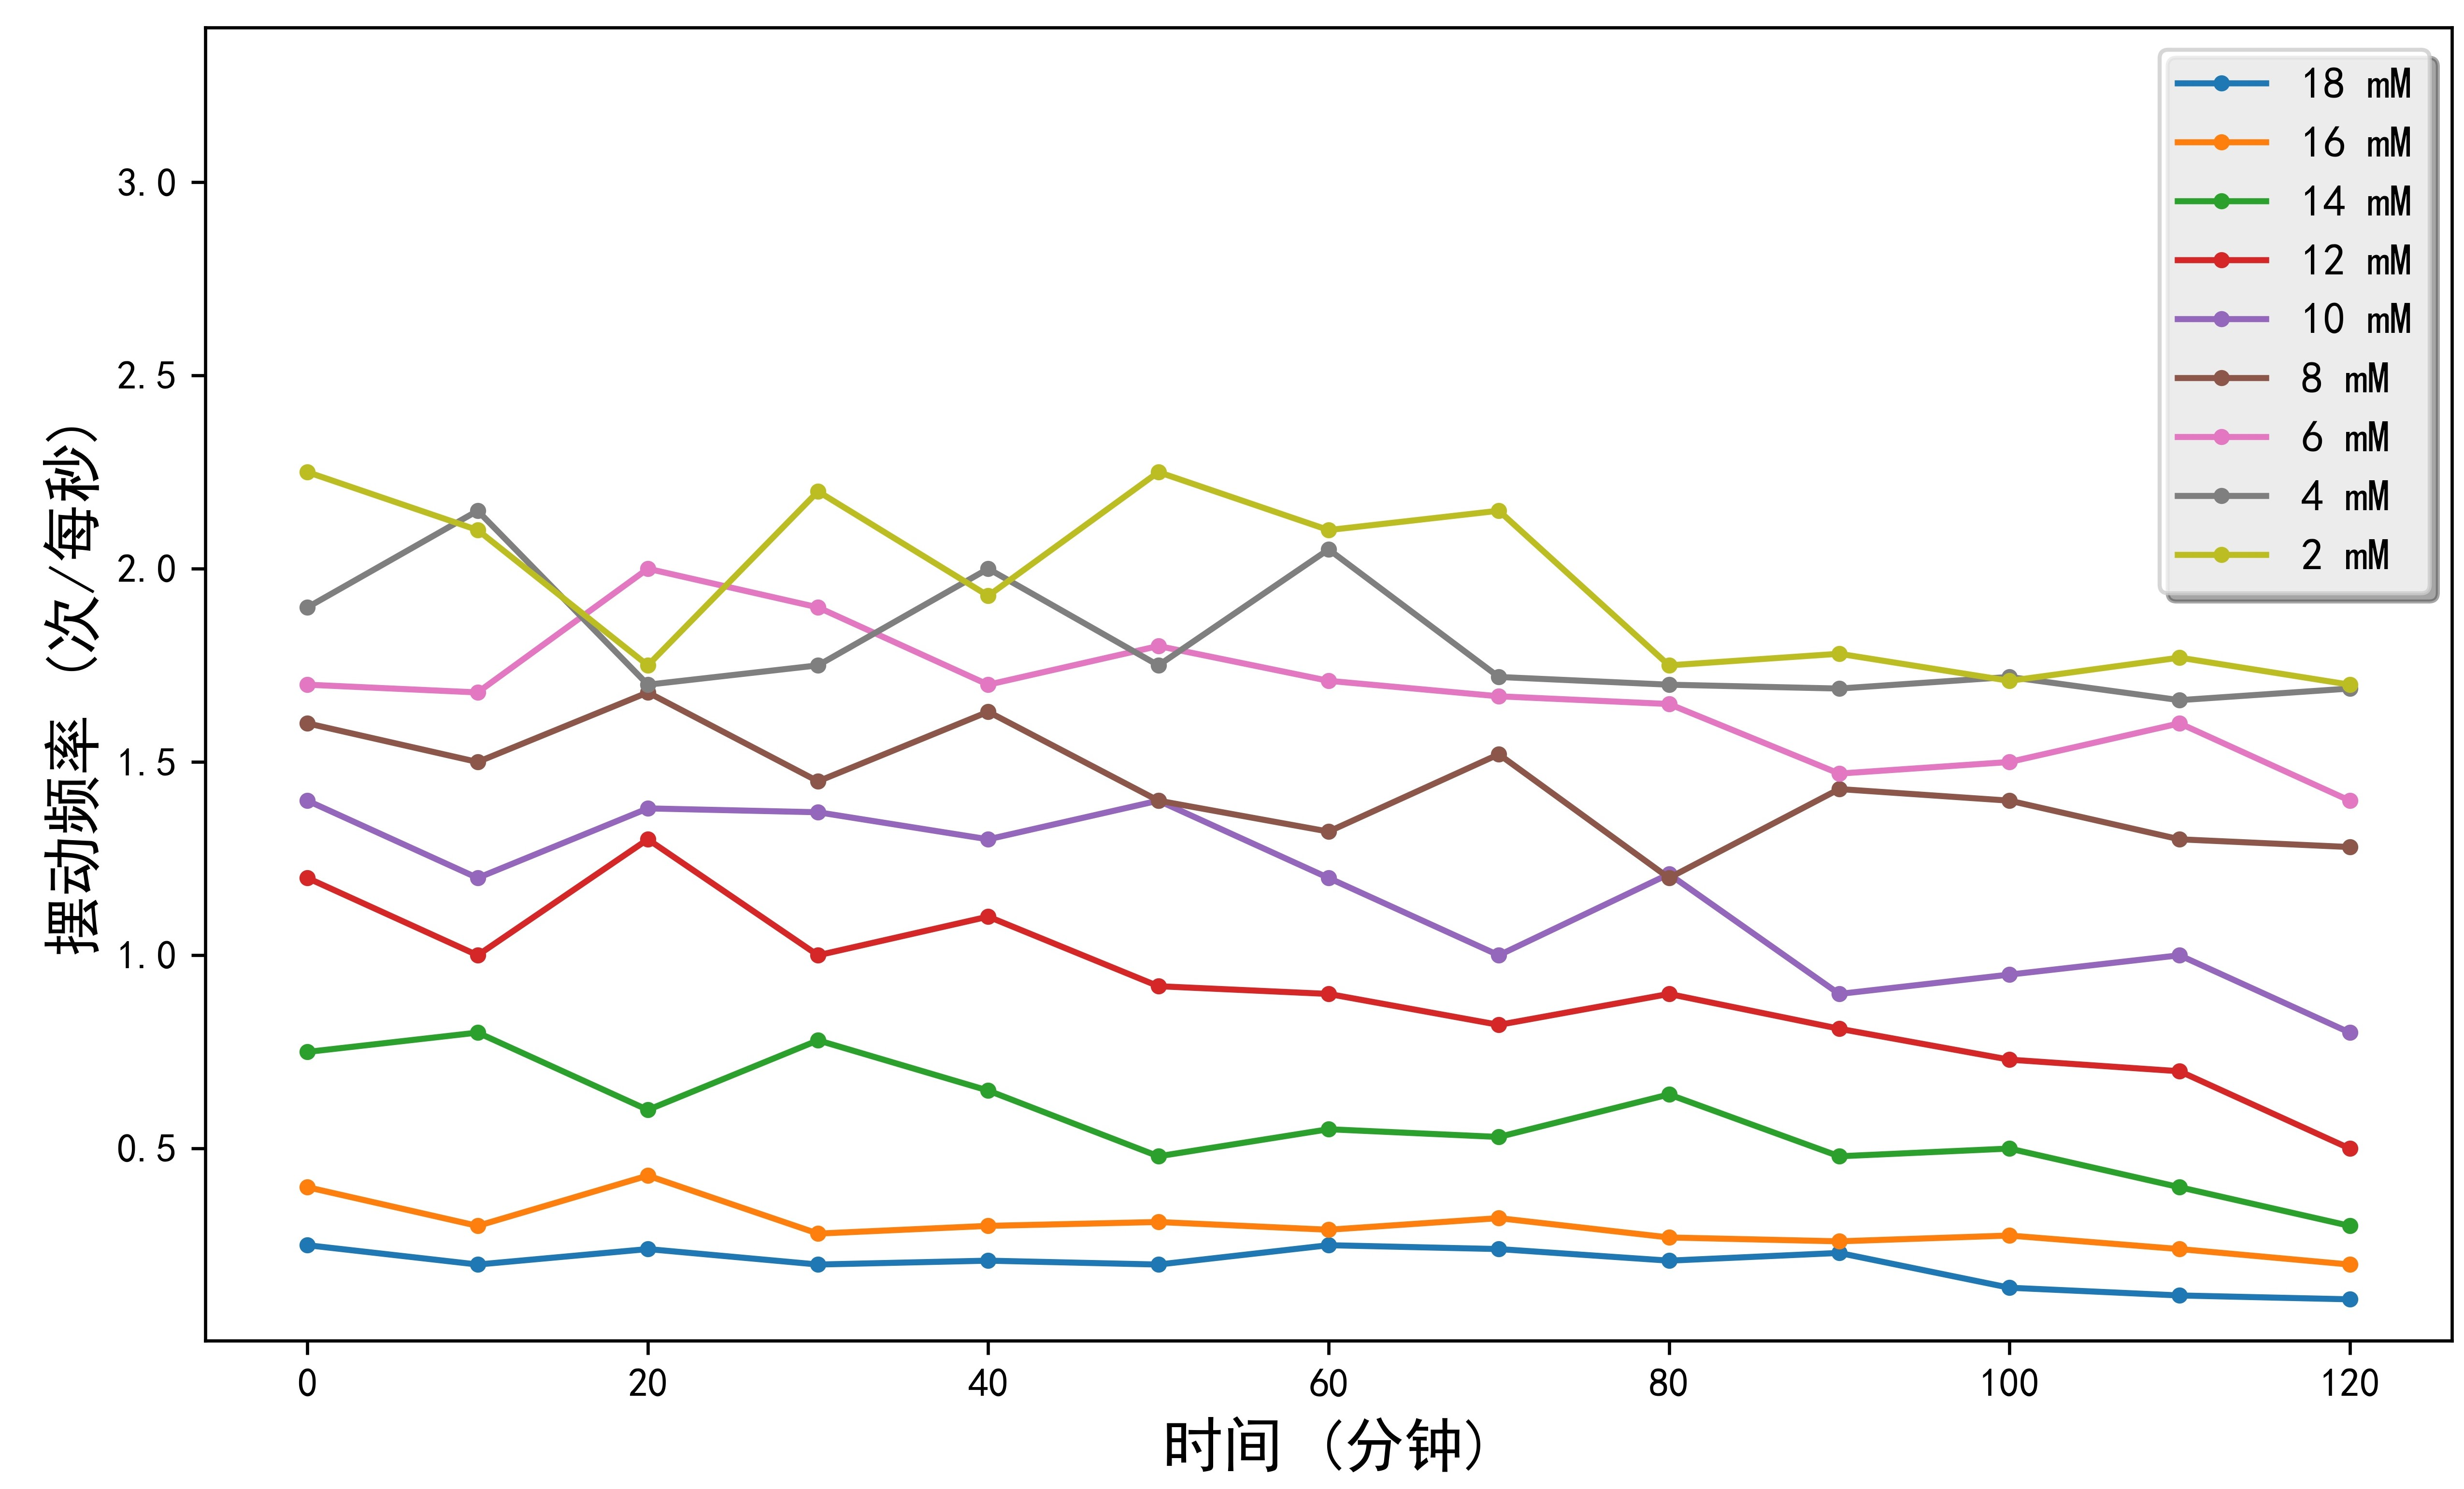
\includegraphics[width=10cm]{figure/chap5/res.jpg}
	  \bicaption[这里将出现在插图索引中]
		{各腔室中线虫平均摆动频率随时间的变化}
		{Change in contour curvature}
	  \label{fig:res}
	\end{figure}
\section{本章小结}
\chapter{总结与展望}
\section{工作总结}
	目前环境中大量的化合物对人类的健康造成了很大的威胁,如何高效快速地评估这些化合物对人类
	健康的影响是目前毒理学研究面临的一个巨大挑战。秀丽隐杆线虫作为一种重要的模式生物,
	在现在毒理学测试中发挥着重要作用。而传统的线虫实验通常在96孔板上完成,需要大量
	的人工操作,不仅操作复杂而且通量低。另一方面,在实验过程中,通过人工观察的方式对线虫相关生理特征
	(如:摆动频率、体长等)的统计,不仅效率低下,而且还会引入人为误差。这些都大大地限制了大规模
	毒理实验的研究进展。本文的工作为基于秀丽隐杆线虫的毒理学测试
	提供了一个集成微流控芯片和自动化视频特征提取的软硬件平台。本文的主要工作如下:
	\begin{enumerate}[label={(\arabic*)},font={\color{black!50!black}\bfseries}]
	\item 本文设计了两款线虫微流控芯片,分别用于线虫急性毒理实验和可以控制线虫
	进样的长期培养芯片。针对用于急性毒理实验的线性浓度梯度稀释芯片,介绍了芯片
	结构设计和双层微流控芯片的制作工艺 (包括芯片模具的制作、微流控芯片的制作等
	工艺步骤),通过染料和荧光实验验证了线性梯度稀释芯片设计的合理性。线性梯度稀释芯
	片虽然在自动化片上梯度形成方面具有优势,但由于没有设计食物供应的通道,因此并
	不适合线虫的长期培养观察,比较适合线虫的急性毒理实验。基于此,本文又设计了一款
	单层带侧向阀门的线虫培养芯片。侧向阀门的设计可以控制腔室中线虫的数量,食物可以
	通过网状结构过滤后流向线虫腔室,为线虫提供食物,虫卵可以通过侧向的管道排出线虫
	培养腔室。从而可以对同一代的线虫进行长期地培养观察。
	\item 基于相机厂商提供的 SDK,开发了一个高速的线虫视频采集程序。
	由于相机的SDK是以动态链接库的形式提供的,而本文将python作为开发语言。
	为了调用相机的API,本文用python的ctypes库对动态链接库中的函数进行了封装以供
	python调用。通过分析了从图像采集到视频写入过
	程中的时间开销,提出了一种多线程的方法将图像采集和视频写入这两个任务并行。
	与单线程的视频采集相比,多线程的方式能够显著提高视频采集的帧率。
	最后测试了不同采集分辨率对视频帧率的影响。
	\item 针对线虫视频特征提取任务的特点,本文采用了“前景轮廓分割——轮廓解析——轮廓跟踪——特征提取”
	的技术路线。针对传统的图像处理方法在线虫前景轮廓分割任务中存在的不足 
	(如:鲁棒性不足、线虫轮廓出现断裂和依赖超参数的选择等),
	本文提出了一种基于条件随机场的深度卷积分割算法,通过与传统的图像分割方法相比,
	本文提出的前景分割算法显著地改善了线虫前景轮廓分割的性能。
针对多线虫轮廓跟踪过程中,多线虫轮廓相互纠缠导致无法区分单个线虫的轮廓,
从而引起线虫轮廓丢失的问题。本文设计了一个基于深度卷积的 
SingleOut-Net 网络,可以成功解析出单个线虫的轮廓,并比较了不同的网络架构
在网络性能、模型复杂度和实时性方面的差异。

	\item 基于线虫轮廓跟踪的结果,本文提出了一种简单有效的线虫轮廓跟踪算法,
	成功实现了对线虫的鲁棒跟踪。该方法首先找出相邻两帧图像中所有线虫轮廓的重心,
	然后通过最近邻匹配的方式找出相邻两帧图像中线虫轮廓之间的对应关系,
	从而实现对线虫轮廓的跟踪。基于线虫轮廓跟踪的结果,本文介绍了线虫轮廓
	中间脊线的提取方法,以及基于线虫的中间脊线介绍了线虫摆动频率和体长的计算方法。
	\end{enumerate}
	
\section{展望}
	本课题拟为基于秀丽隐杆线虫的大规模毒理学测试和药物筛选搭建一个软硬件平台。
	在芯片操作方面,该平台可以实现线虫的长期培养、自动给药、片上梯度形成等
	自动化操作。在生理特征检测方面,该平台可以实现体长、身体弯曲频率、头部
	摆动频率、产卵率等生理特征的监测。但限于时间关系,本文的工作并没有将
	这些功能全部包括。结合本文已经完成的工作,未来该平台可以在以下几个方面进一步优化:
	
	\begin{enumerate}[label={(\arabic*)},font={\color{black!50!black}\bfseries}]
	\item 线虫产卵率的监测对于生殖毒性的评价而言,是非常重要的指标。
	下一阶段可以考虑在芯片设计和虫卵识别计数两个方面开展工作。在芯
	片设计方面,可以设计一款具备将线虫和虫卵分离同时将虫卵收集在一个
	腔室功能的芯片,并通过图像识别算法对这个腔室中的虫卵进行计数。
	\item 在神经发育毒性的评价中,头部摆动频率也是一项十分重要的指标。
	现阶段本平台已经具备了对线虫进行前景轮廓分割、轮廓解析、轮廓跟踪、
	线虫轮廓中间脊线提取和线虫身体弯曲频率计算等功能。下一阶段,
	可以基于目前线虫轮廓中间脊线的提取结果完成头部摆动频率的计算。
	\item 在芯片设计上,充分利用微流控芯片高通量的优势。
	下一阶段的工作可以考虑设计具备形成多种化合物复合浓度梯度功能的线虫芯片,
	同时该芯片上应包含更多的线虫培养腔室。进一步体现该平台在复合药物毒性评价方面
	高通量的优势。
	\item 为了探索毒性标志,未来可以将线虫微流控芯片和质谱仪连接,对线虫的代谢产物进行毒性鉴别。

	\end{enumerate}









%%# -*- coding: utf-8-unix -*-
% !TEX program = xelatex
% !TEX root = ../thesis.tex
% !TEX encoding = UTF-8 Unicode
%%==================================================
%% chapter02.tex for SJTU Master Thesis
%% based on CASthesis
%% modified by wei.jianwen@gmail.com
%% Encoding: UTF-8
%%==================================================

\chapter{{\LaTeX} 排版例子}
\label{chap:example}
%%%%%%%%%%%%%%%%%%%%%%%%%%%%%%%%%%%%%%%%%%%%%%%%%%%%%%%%%%%%%%%%%%%%%%%%%%%%%%%%%%%%%%%%%%%%%%%%%%%%%%%%%
\section{列表环境}
\label{sec:list}

\subsection{无序列表}
\label{sec:unorderlist}

以下是一个无序列表的例子,列表的每个条目单独分段。

\begin{itemize}
  \item 这是一个无序列表。
  \item 这是一个无序列表。
  \item 这是一个无序列表。
\end{itemize}

使用\verb+itemize*+环境可以创建行内无序列表。
\begin{itemize*}
  \item 这是一个无序列表。
  \item 这是一个无序列表。
  \item 这是一个无序列表。
\end{itemize*}
行内无序列表条目不单独分段,所有内容直接插入在原文的段落中。

\subsection{有序列表}
\label{sec:orderlist}

使用环境\verb+enumerate+和\verb+enumerate*+创建有序列表,
使用方法无序列表类似。

\begin{enumerate}
  \item 这是一个有序列表。
  \item 这是一个有序列表。
  \item 这是一个有序列表。
\end{enumerate}

使用\verb+enumerate*+环境可以创建行内有序列表。
\begin{enumerate*}
  \item 这是一个默认有序列表。
  \item 这是一个默认有序列表。
  \item 这是一个默认有序列表。
\end{enumerate*}
行内有序列表条目不单独分段,所有内容直接插入在原文的段落中。

\subsection{描述型列表}

使用环境\verb+description+可创建带有主题词的列表,条目语法是\verb+\item[主题] 内容+。
\begin{description}
    \item[主题一] 详细内容
    \item[主题二] 详细内容
    \item[主题三] 详细内容 \ldots
\end{description}

\subsection{自定义列表样式}

可以使用\verb+label+参数控制列表的样式,
详细可以参考WikiBooks\footnote{\url{https://en.wikibooks.org/wiki/LaTeX/List_Structures\#Customizing_lists}}。
比如一个自定义样式的行内有序列表
\begin{enumerate*}[label=\itshape\alph*)\upshape]
  \item 这是一个自定义样式有序列表。
  \item 这是一个自定义样式有序列表。
  \item 这是一个自定义样式有序列表。
\end{enumerate*}
%%%%%%%%%%%%%%%%%%%%%%%%%%%%%%%%%%%%%%%%%%%%%%%%%%%%%%%%%%%%%%%%%%%%%%%%%%%%%%%%%%%%%%%%%%%%%%%%%%%%%%%%%%
\section{数学排版}
\label{sec:matheq}

\subsection{公式排版}
\label{sec:eqformat}

这里有举一个长公式排版的例子,来自\href{http://www.tex.ac.uk/tex-archive/info/math/voss/mathmode/Mathmode.pdf}{《Math mode》}:

\begin {multline}
  \frac {1}{2}\Delta (f_{ij}f^{ij})=
  2\left (\sum _{i<j}\chi _{ij}(\sigma _{i}-
    \sigma _{j}) ^{2}+ f^{ij}\nabla _{j}\nabla _{i}(\Delta f)+\right .\\
  \left .+\nabla _{k}f_{ij}\nabla ^{k}f^{ij}+
    f^{ij}f^{k}\left [2\nabla _{i}R_{jk}-
      \nabla _{k}R_{ij}\right ]\vphantom {\sum _{i<j}}\right )
\end{multline}

\subsection{SI单位}

使用\verb+siunitx+宏包可以方便地输入SI单位制单位,例如\verb+\SI{5}{\um}+可以得到\SI{5}{\um}。

\subsubsection{一个四级标题}
\label{sec:depth4}

这是全文唯一的一个四级标题。在这部分中将演示了mathtools宏包中可伸长符号(箭头、等号的例子)的例子。

\begin{displaymath}
    A \xleftarrow[n=0]{} B \xrightarrow[LongLongLongLong]{n>0} C
\end{displaymath}

\begin{eqnarray}
  f(x) & \xleftrightarrow[]{A=B}  & B \\
  & \xleftharpoondown[below]{above} & B \nonumber \\
  & \xLeftrightarrow[below]{above} & B
\end{eqnarray}

又如:

\begin{align}
  \label{eq:none}
  & I(X_3;X_4)-I(X_3;X_4\mid{}X_1)-I(X_3;X_4\mid{}X_2) \nonumber \\
  = & [I(X_3;X_4)-I(X_3;X_4\mid{}X_1)]-I(X_3;X_4\mid{}\tilde{X}_2) \\
  = & I(X_1;X_3;X_4)-I(X_3;X_4\mid{}\tilde{X}_2)
\end{align}

\subsection{定理环境}

模板中定义了丰富的定理环境
algo(算法),thm(定理),lem(引理),prop(命题),cor(推论),defn(定义),conj(猜想),exmp(例),rem(注),case(情形),
bthm(断言定理),blem(断言引理),bprop(断言命题),bcor(断言推论)。
amsmath还提供了一个proof(证明)的环境。
这里举一个“定理”和“证明”的例子。
\begin{thm}[留数定理]
\label{thm:res}
  假设$U$是复平面上的一个单连通开子集,$a_1,\ldots,a_n$是复平面上有限个点,$f$是定义在$U\backslash \{a_1,\ldots,a_n\}$上的全纯函数,
  如果$\gamma$是一条把$a_1,\ldots,a_n$包围起来的可求长曲线,但不经过任何一个$a_k$,并且其起点与终点重合,那么:

  \begin{equation}
    \label{eq:res}
    \ointop_{\gamma}f(z)\,\mathrm{d}z = 2\uppi\mathbf{i}\sum^n_{k=1}\mathrm{I}(\gamma,a_k)\mathrm{Res}(f,a_k)
  \end{equation}

  如果$\gamma$是若尔当曲线,那么$\mathrm{I}(\gamma, a_k)=1$,因此:

  \begin{equation}
    \label{eq:resthm}
    \ointop_{\gamma}f(z)\,\mathrm{d}z = 2\uppi\mathbf{i}\sum^n_{k=1}\mathrm{Res}(f,a_k)
  \end{equation}

      % \oint_\gamma f(z)\, dz = 2\pi i \sum_{k=1}^n \mathrm{Res}(f, a_k ).

  在这里,$\mathrm{Res}(f, a_k)$表示$f$在点$a_k$的留数,$\mathrm{I}(\gamma,a_k)$表示$\gamma$关于点$a_k$的卷绕数。
  卷绕数是一个整数,它描述了曲线$\gamma$绕过点$a_k$的次数。如果$\gamma$依逆时针方向绕着$a_k$移动,卷绕数就是一个正数,
  如果$\gamma$根本不绕过$a_k$,卷绕数就是零。

  定理\ref{thm:res}的证明。

  \begin{proof}
    首先,由……

    其次,……

    所以……
  \end{proof}
\end{thm}

上面的公式例子中,有一些细节希望大家注意。微分号d应该使用“直立体”也就是用mathrm包围起来。
并且,微分号和被积函数之间应该有一段小间隔,可以插入\verb+\,+得到。
斜体的$d$通常只作为一般变量。
i,j作为虚数单位时,也应该使用“直立体”为了明显,还加上了粗体,例如\verb+\mathbf{i}+。斜体$i,j$通常用作表示“序号”。
其他字母在表示常量时,也推荐使用“直立体”譬如,圆周率$\uppi$(需要upgreek宏包),自然对数的底$\mathrm{e}$。
不过,我个人觉得斜体的$e$和$\pi$很潇洒,在不至于引起混淆的情况下,我也用这两个字母的斜体表示对应的常量。

%%%%%%%%%%%%%%%%%%%%%%%%%%%%%%%%%%%%%%%%%%%%%%%%%%%%%%%%%%%%%%%%%%%%%%%%%%%%%%%%%%%%%%%%%%%%%%%%%%%%%%%%%%%%%%%%%%
\section{向文档中插入图像}
\label{sec:insertimage}

\subsection{支持的图片格式}
\label{sec:imageformat}

\XeTeX 可以很方便地插入PDF、PNG、JPG格式的图片。

插入PNG/JPG的例子如\ref{fig:SRR}所示。
这两个水平并列放置的图共享一个“图标题”(table caption),没有各自的小标题。

\begin{figure}[!htp]
  \centering
  
\includegraphics[width=4cm]{example/sjtulogo.png}
  \hspace{1cm}
  
\includegraphics[width=4cm]{example/sjtulogo.jpg}
  \bicaption[这里将出现在插图索引中]
    {中文题图}
    {English caption}
  \label{fig:SRR}
\end{figure}

这里还有插入EPS图像和PDF图像的例子,如图\ref{fig:epspdf:a}和图\ref{fig:epspdf:b}。这里将EPS和PDF图片作为子图插入,每个子图有自己的小标题。子图标题使用subcaption宏包添加。

\begin{figure}[!htp]
  \centering
  \subcaptionbox{EPS 图像\label{fig:epspdf:a}}[3cm] %标题的长度,超过则会换行,如下一个小图。
    {
\includegraphics[height=2.5cm]{example/sjtulogo.eps}}
  \hspace{4em}
  \subcaptionbox{PDF 图像,注意这个图略矮些。如果标题很长的话,它会自动换行\label{fig:epspdf:b}}
    {
\includegraphics[height=2cm]{sjtulogo.pdf}}
  \bicaption{插入eps和pdf的例子(使用 subcaptionbox 方式)}{An EPS and PDF demo with subcaptionbox}
  \label{fig:pdfeps-subcaptionbox}
\end{figure}

\begin{figure}[!htp]
  \centering
  \begin{subfigure}{2.5cm}
    \centering
    
\includegraphics[height=2.5cm]{example/sjtulogo.eps}
    \caption{EPS 图像}
  \end{subfigure}
  \hspace{4em}
  \begin{subfigure}{0.4\textwidth}
    \centering
    
\includegraphics[height=2cm]{sjtulogo.pdf}
    \caption{PDF 图像,注意这个图略矮些。subfigure中同一行的子图在顶端对齐。}
  \end{subfigure}
  \bicaption{插入eps和pdf的例子(使用 subfigure 方式)}{An EPS and PDF demo with subfigure}
  \label{fig:pdfeps-subfigure}
\end{figure}

更多关于 \LaTeX 插图的例子可以参考\href{http://www.cs.duke.edu/junhu/Graphics3.pdf}{《\LaTeX 插图指南》}。

\subsection{长标题的换行}
\label{sec:longcaption}

图\ref{fig:longcaptionbad}和图\ref{fig:longcaptiongood}都有比较长图标题,通过对比发现,图\ref{fig:longcaptiongood}的换行效果更好一些。
其中使用了minipage环境来限制整个浮动体的宽度。

\begin{figure}[!htp]
  \centering
  
\includegraphics[width=4cm]{sjtubadge.pdf}
  \bicaption[这里将出现在插图索引]
    {上海交通大学是我国历史最悠久的高等学府之一,是教育部直属、教育部与上海市共建的全国重点大学.}
    {Where there is a will, there is a way.}
 \label{fig:longcaptionbad}
\end{figure}

\begin{figure}[!htbp]
  \centering
  \begin{minipage}[b]{0.6\textwidth}
    \centering
    
\includegraphics[width=4cm]{sjtubadge.pdf}
    \bicaption[出现在插图索引中]
      {上海交通大学是我国历史最悠久的高等学府之一,是教育部直属、教育部与上海市共建的全国重点大学.}
      {Where there is a will, there is a way.}
    \label{fig:longcaptiongood}
  \end{minipage}
\end{figure}

\subsection{添加图注}

当插图中组成部件由数字或字母等编号表示时,可在插图下方添加图注进行说明,如图\ref{fig:cn_100t}所示。

\begin{figure}[!htp]
  \centering
  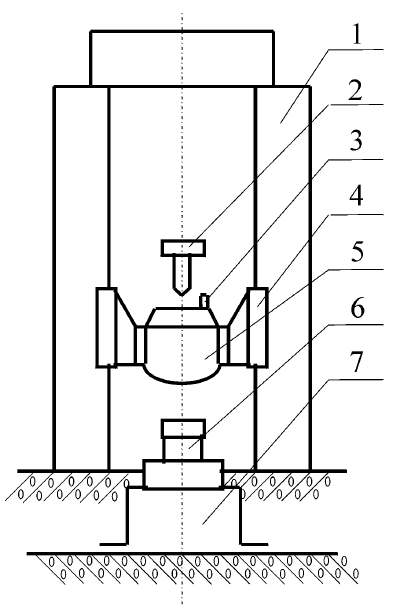
\includegraphics[width=0.3\textwidth]{example/cn_100t.png}\
  \begin{center}
    \small\kaishu 1.立柱 2.提升释放机构 3.标准冲击加速度计 \\ 4.导轨 5.重锤 6.被校力传感器 7.底座
  \end{center}
  \vspace{-1em}
  \bicaption[出现在插图索引中]
    {示例图片来源于\parencite{he1999}}
    {Stay hungry, stay foolish.}
 \label{fig:cn_100t}
\end{figure}

\subsection{绘制流程图}

图\ref{fig:flow_chart}是一张流程图示意。使用tikz环境,搭配四种预定义节点(\verb+startstop+、\verb+process+、\verb+decision+和\verb+io+),可以容易地绘制出流程图。
\begin{figure}[!htp]
    \centering
    \resizebox{6cm}{!}{\begin{tikzpicture}[node distance=2cm]
    \node (pic) [startstop] {待测图片};
    \node (bg) [io, below of=pic] {读取背景};
    \node (pair) [process, below of=bg] {匹配特征点对};
    \node (threshold) [decision, below of=pair, yshift=-0.5cm] {多于阈值};
    \node (clear) [decision, right of=threshold, xshift=3cm] {清晰?};
    \node (capture) [process, right of=pair, xshift=3cm, yshift=0.5cm] {重采};
    \node (matrix_p) [process, below of=threshold, yshift=-0.8cm] {透视变换矩阵};
    \node (matrix_a) [process, right of=matrix_p, xshift=3cm] {仿射变换矩阵};
    \node (reg) [process, below of=matrix_p] {图像修正};
    \node (return) [startstop, below of=reg] {配准结果};
     
    %连接具体形状
    \draw [arrow](pic) -- (bg);
    \draw [arrow](bg) -- (pair);
    \draw [arrow](pair) -- (threshold);

    \draw [arrow](threshold) -- node[anchor=south] {否} (clear);

    \draw [arrow](clear) -- node[anchor=west] {否} (capture);
    \draw [arrow](capture) |- (pic);
    \draw [arrow](clear) -- node[anchor=west] {是} (matrix_a);
    \draw [arrow](matrix_a) |- (reg);

    \draw [arrow](threshold) -- node[anchor=east] {是} (matrix_p);
    \draw [arrow](matrix_p) -- (reg);
    \draw [arrow](reg) -- (return);
\end{tikzpicture}
}
    \bicaption{绘制流程图效果}{Flow chart}
    \label{fig:flow_chart}
\end{figure}

\clearpage

\section{表格}
\label{sec:tab}

这一节给出的是一些表格的例子,如表\ref{tab:firstone}所示。

\begin{table}[!hpb]
  \centering
  \bicaption[指向一个表格的表目录索引]
    {一个颇为标准的三线表格\footnotemark[1]}
    {A Table}
  \label{tab:firstone}
  \begin{tabular}{@{}llr@{}} \toprule
    \multicolumn{2}{c}{Item} \\ \cmidrule(r){1-2}
    Animal & Description & Price (\$)\\ \midrule
    Gnat & per gram & 13.65 \\
    & each & 0.01 \\
    Gnu & stuffed & 92.50 \\
    Emu & stuffed & 33.33 \\
    Armadillo & frozen & 8.99 \\ \bottomrule
  \end{tabular}
\end{table}
\footnotetext[1]{这个例子来自\href{http://www.ctan.org/tex-archive/macros/latex/contrib/booktabs/booktabs.pdf}{《Publication quality tables in LATEX》}(booktabs宏包的文档)。这也是一个在表格中使用脚注的例子,请留意与threeparttable实现的效果有何不同。}

下面一个是一个更复杂的表格,用threeparttable实现带有脚注的表格,如表\ref{tab:footnote}。

\begin{table}[!htpb]
  \bicaption[出现在表目录的标题]
    {一个带有脚注的表格的例子}
    {A Table with footnotes}
  \label{tab:footnote}
  \centering
  \begin{threeparttable}[b]
     \begin{tabular}{ccd{4}cccc}
      \toprule
      \multirow{2}{6mm}{total}&\multicolumn{2}{c}{20\tnote{1}} & \multicolumn{2}{c}{40} &  \multicolumn{2}{c}{60}\\
      \cmidrule(lr){2-3}\cmidrule(lr){4-5}\cmidrule(lr){6-7}
      &www & \multicolumn{1}{c}{k} & www & k & www & k \\ % 使用说明符 d 的列会自动进入数学模式,使用 \multicolumn 对文字表头做特殊处理
      \midrule
      &$\underset{(2.12)}{4.22}$ & 120.0140\tnote{2} & 333.15 & 0.0411 & 444.99 & 0.1387 \\
      &168.6123 & 10.86 & 255.37 & 0.0353 & 376.14 & 0.1058 \\
      &6.761    & 0.007 & 235.37 & 0.0267 & 348.66 & 0.1010 \\
      \bottomrule
    \end{tabular}
    \begin{tablenotes}
    \item [1] the first note.% or \item [a]
    \item [2] the second note.% or \item [b]
    \end{tablenotes}
  \end{threeparttable}
\end{table}

\section{参考文献管理}

 \LaTeX 具有将参考文献内容和表现形式分开管理的能力,涉及三个要素:参考文献数据库、参考文献引用格式、在正文中引用参考文献。
这样的流程需要多次编译:

\begin{enumerate}[noitemsep,topsep=0pt,parsep=0pt,partopsep=0pt]
	\item 用户将论文中需要引用的参考文献条目,录入纯文本数据库文件(bib文件)。
	\item 调用xelatex对论文模板做第一次编译,扫描文中引用的参考文献,生成参考文献入口文件(aux)文件。
	\item 调用bibtex,以参考文献格式和入口文件为输入,生成格式化以后的参考文献条目文件(bib)。
	\item 再次调用xelatex编译模板,将格式化以后的参考文献条目插入正文。
\end{enumerate}

参考文献数据库(thesis.bib)的条目,可以从Google Scholar搜索引擎\footnote{\url{https://scholar.google.com}}、CiteSeerX搜索引擎\footnote{\url{http://citeseerx.ist.psu.edu}}中查找,文献管理软件Papers\footnote{\url{http://papersapp.com}}、Mendeley\footnote{\url{http://www.mendeley.com}}、JabRef\footnote{\url{http://jabref.sourceforge.net}}也能够输出条目信息。

下面是在Google Scholar上搜索到的一条文献信息,格式是纯文本:

\begin{lstlisting}[caption={从Google Scholar找到的参考文献条目}, label=googlescholar, escapeinside="", numbers=none]
    @phdthesis{"白2008信用风险传染模型和信用衍生品的定价",
      title={"信用风险传染模型和信用衍生品的定价"},
      author={"白云芬"},
      year={2008},
      school={"上海交通大学"}
    }
\end{lstlisting}

推荐修改后在bib文件中的内容为:

\begin{lstlisting}[caption={修改后的参考文献条目}, label=itemok, escapeinside="", numbers=none]
  @phdthesis{bai2008,
    title={"信用风险传染模型和信用衍生品的定价"},
    author={"白云芬"},
    date={2008},
    address={"上海"},
    school={"上海交通大学"}
  }
\end{lstlisting}

按照教务处的要求,参考文献外观应符合国标GBT7714的要求\footnote{\url{http://www.cces.net.cn/guild/sites/tmxb/Files/19798_2.pdf}}。
在模板中,表现形式的控制逻辑通过biblatex-gb7714-2015包实现\footnote{\url{https://www.ctan.org/pkg/biblatex-gb7714-2015}},基于{Bib\LaTeX}管理文献。在目前的多数TeX发行版中,可能都没有默认包含biblatex-gb7714-2015,需要手动安装。

正文中引用参考文献时,用\verb+\cite{key1,key2,key3...}+可以产生“上标引用的参考文献”,
如\cite{Meta_CN,chen2007act,DPMG}。
使用\verb+\parencite{key1,key2,key3...}+则可以产生水平引用的参考文献,例如\parencite{JohnD,zhubajie,IEEE-1363}。
请看下面的例子,将会穿插使用水平的和上标的参考文献:关于书的\parencite{Meta_CN,JohnD,IEEE-1363},关于期刊的\cite{chen2007act,chen2007ewi},
会议论文\parencite{DPMG,kocher99,cnproceed},
硕士学位论文\parencite{zhubajie,metamori2004},博士学位论文\cite{shaheshang,FistSystem01,bai2008},标准文件\parencite{IEEE-1363},技术报告\cite{NPB2},电子文献\parencite{xiaoyu2001, CHRISTINE1998},用户手册\parencite{RManual}。

总结一些注意事项:
\begin{itemize}
\item 参考文献只有在正文中被引用了,才会在最后的参考文献列表中出现;
\item 参考文献“数据库文件”bib是纯文本文件,请使用UTF-8编码,不要使用GBK编码;
\item 参考文献条目中默认通过date域输入时间。兼容使用year域时会产生编译warning,可忽略。
\end{itemize}

\section{用listings插入源代码}

原先ctexbook文档类和listings宏包配合使用时,代码在换页时会出现莫名其妙的错误,后来经高人指点,顺利解决了。
感兴趣的话,可以看看\href{http://bbs.ctex.org/viewthread.php?tid=53451}{这里}。
这里给使用listings宏包插入源代码的例子,这里是一段C代码。
另外,listings宏包真可谓博大精深,可以实现各种复杂、漂亮的效果,想要进一步学习的同学,可以参考
\href{http://mirror.ctan.org/macros/latex/contrib/listings/listings.pdf}{listings宏包手册}。

\begin{lstlisting}[language={C}, caption={一段C源代码}]
#include <stdio.h>
#include <unistd.h>
#include <sys/types.h>
#include <sys/wait.h>

int main() {
  pid_t pid;

  switch ((pid = fork())) {
  case -1:
    printf("fork failed\n");
    break;
  case 0:
    /* child calls exec */
    execl("/bin/ls", "ls", "-l", (char*)0);
    printf("execl failed\n");
    break;
  default:
    /* parent uses wait to suspend execution until child finishes */
    wait((int*)0);
    printf("is completed\n");
    break;
  }

  return 0;
}
\end{lstlisting}

\section{用algorithm和algorithmicx宏包插入算法描述}

algorithmicx 比 algorithmic 增加了一些命令。
示例如算法\ref{algo:sum_100}和算法\ref{algo:merge_sort},
后者的代码来自\href{http://hustsxh.is-programmer.com/posts/38801.html}{xhSong的博客}。
algorithmicx的详细使用方法见\href{http://mirror.hust.edu.cn/CTAN/macros/latex/contrib/algorithmicx/algorithmicx.pdf}{官方README}。
使用算法宏包时,算法出现的位置很多时候不按照tex文件里的书写顺序,
需要强制定位时可以使用\verb+\begin{algorithm}[H]+
\footnote{http://tex.stackexchange.com/questions/165021/fixing-the-location-of-the-appearance-in-algorithmicx-environment}

这是写在算法\ref{algo:sum_100}前面的一段话,在生成的文件里它会出现在算法\ref{algo:sum_100}前面。

\begin{algorithm}
% \begin{algorithm}[H] % 强制定位
\caption{求100以内的整数和}
\label{algo:sum_100}
\begin{algorithmic}[1] %每行显示行号
\Ensure 100以内的整数和 % 输出
\State $sum \gets 0$
\For{$i = 0 \to 100$}
    \State $sum \gets sum + i$
  \EndFor
\end{algorithmic}
\end{algorithm}

这是写在两个算法中间的一段话,当算法\ref{algo:sum_100}不使用\verb+\begin{algorithm}[H]+时它也会出现在算法\ref{algo:sum_100}前面。

对于很长的算法,单一的算法块\verb+\begin{algorithm}...\end{algorithm}+是不能自动跨页的
\footnote{http://tex.stackexchange.com/questions/70733/latex-algorithm-not-display-under-correct-section},
会出现的情况有:

\begin{itemize}
  \item 该页放不下当前的算法,留下大片空白,算法在下一页显示
  \item 单一页面放不下当前的算法,显示时超过页码的位置直到超出整个页面范围
\end{itemize}

解决方法有:

\begin{itemize}
  \item (推荐)使用\verb+algstore{algname}+和\verb+algrestore{algname}+来讲算法分为两个部分\footnote{http://tex.stackexchange.com/questions/29816/algorithm-over-2-pages},如算法\ref{algo:merge_sort}。
  \item 人工拆分算法为多个小的部分。
\end{itemize}

\begin{algorithm}
% \begin{algorithm}[H] % 强制定位
\caption{用归并排序求逆序数}
\label{algo:merge_sort}
\begin{algorithmic}[1] %每行显示行号
\Require $Array$数组,$n$数组大小 % 输入
\Ensure 逆序数 % 输出
\Function {MergerSort}{$Array, left, right$}
  \State $result \gets 0$
  \If {$left < right$}
    \State $middle \gets (left + right) / 2$
    \State $result \gets result +$ \Call{MergerSort}{$Array, left, middle$}
    \State $result \gets result +$ \Call{MergerSort}{$Array, middle, right$}
    \State $result \gets result +$ \Call{Merger}{$Array,left,middle,right$}
  \EndIf
  \State \Return{$result$}
\EndFunction
\State %空一行
\Function{Merger}{$Array, left, middle, right$}
  \State $i\gets left$
  \State $j\gets middle$
  \State $k\gets 0$
  \State $result \gets 0$
  \While{$i<middle$ \textbf{and} $j<right$}
    \If{$Array[i]<Array[j]$}
      \State $B[k++]\gets Array[i++]$
    \Else
      \State $B[k++] \gets Array[j++]$
      \State $result \gets result + (middle - i)$
    \EndIf
  \EndWhile
  \algstore{MergeSort}
\end{algorithmic}
\end{algorithm}

\begin{algorithm}
\begin{algorithmic}[1]
  \algrestore{MergeSort}
  \While{$i<middle$}
    \State $B[k++] \gets Array[i++]$
  \EndWhile
  \While{$j<right$}
    \State $B[k++] \gets Array[j++]$
  \EndWhile
  \For{$i = 0 \to k-1$}
    \State $Array[left + i] \gets B[i]$
  \EndFor
  \State \Return{$result$}
\EndFunction
\end{algorithmic}
\end{algorithm}

这是写在算法\ref{algo:merge_sort}后面的一段话,
但是当算法\ref{algo:merge_sort}不使用\verb+\begin{algorithm}[H]+时它会出现在算法\ref{algo:merge_sort}
甚至算法\ref{algo:sum_100}前面。

对于算法的索引要注意\verb+\caption+和\verb+\label+的位置,
必须是先\verb+\caption+再\verb+\label+\footnote{http://tex.stackexchange.com/questions/65993/algorithm-numbering},
否则会出现\verb+\ref{algo:sum_100}+生成的编号跟对应算法上显示不一致的问题。

根据Werner的回答\footnote{http://tex.stackexchange.com/questions/53357/switch-cases-in-algorithmic}
增加了\verb+Switch+和\verb+Case+的支持,见算法\ref{algo:switch_example}。

\begin{algorithm}
\caption{Switch示例}
\label{algo:switch_example}
\begin{algorithmic}[1]
  \Switch{$s$}
    \Case{$a$}
      \Assert{0}
    \EndCase
    \Case{$b$}
      \Assert{1}
    \EndCase
    \Default
      \Assert{2}
    \EndDefault
  \EndSwitch
\end{algorithmic}
\end{algorithm}

%%# -*- coding: utf-8-unix -*-
% !TEX program = xelatex
% !TEX root = ../thesis.tex
% !TEX encoding = UTF-8 Unicode
\chapter{常见问题}
\label{chap:faq}

{\bfseries{}Q:我是否能够自由使用这份模板?}

A:这份模板以Apache License 2.0开源许可证发布,请遵循许可证规范。

{\bfseries{}Q:我的论文是Word排版的,学校图书馆是不是只收 \LaTeX 排版的论文?}

A:当然不是,Word版论文肯定收。

{\bfseries{}Q:我的论文是 \LaTeX 排版的,学校图书馆是不是只收Word排版的论文?}

A:当然不是,PDF版的电子论文是可以上交的。是否要交Word版就看你导师的喜好了。

{\bfseries{}Q:为什么屏幕上显示的左右页边距不一样?}

A:模板默认是双面打印,迎面页和背面页的页边距是要交换的,多出来的那一部分是留作装订的。

{\bfseries{}Q:为什么在参考文献中会有“//”符号?}

A:那就是国标GBT7714参考文献风格规定的。但可以使用 gbpunctin=false 选项将其还原成 in:,进一步可以在导言区加入\verb+\DefineBibliographyStrings{english}{in={}}+将其去掉。

{\bfseries{}Q:为什么参考文献中会有[s.n.],[S.l], [EB/OL]等符号?}

A: 那也是国标GBT7714参考文献风格定义的。[s.n.]表示出版者不祥,[S.l]表示出版地不祥,[EB/OL]表示引用的参考文献类型为在线电子文档。但可以使用gbpub=false 选项将其缺省补充的出版项[s.n.]等去掉。也可以使用选项 gbtype=false 将参考文献类型标识去掉。

{\bfseries{}Q:如何获得帮助和反馈意见?}

A:你可以通过\href{https://github.com/sjtug/SJTUThesis/issues}{在github上开issue}
、在\href{https://bbs.sjtu.edu.cn/bbsdoc?board=TeX_LaTeX}{水源LaTeX版}发帖反映你使用过程中遇到的问题。

{\bfseries{}Q:使用文本编辑器查看tex文件时遇到乱码?}

A:请确保你的文本编辑器使用UTF-8编码打开了tex源文件。

{\bfseries{}Q:在CTeX编译模板遇到“rsfs10.tfm already exists”的错误提示?}

A:请删除\verb+X:\CTEX\UserData\fonts\tfm\public\rsfs+下的文件再重新编译。问题讨论见\href{https://bbs.sjtu.edu.cn/bbstcon,board,TeX_LaTeX,reid,1352982719.html}{水源2023号帖}。

{\bfseries{}Q:升级了TeXLive 2012,编译后的文档出现“minus”等字样?}

A:这是xltxtra和fontspec宏包导致的问题。学位论文模板从0.5起使用metatlog宏包代替xltxtra生成 \XeTeX 标志,解决了这个问题。

{\bfseries{}Q:为什么在bib中加入的参考文献,没有在参考文献列表中出现?}

A: bib中的参考文献条目,常通过\verb+\cite+或\verb+\parencite+或\verb+\supercite+或\verb+\textcite+等命令在正文中引用进而加入到参考文献列表中。当需要将参考文献条目加入到文献表中但又不引用可以使用\verb+\nocite+命令,当nocite参数为*时则引入bib中的所有文献。
%\verb+\upcite+ 是哪个宏包的?之前没有见过

{\bfseries{}Q:我可以使用Sublime Text编写学位论文吗?}

A: 可以。首先\href{https://www.sublimetext.com/}{下载}并安装Sublime Text,然后安装
\href{https://packagecontrol.io/installation}{Package Control},
之后按\verb|ctrl+shift+p|或者\verb|cmd+shift+p|调出命令窗口,
输入\verb|install|,选择\textit{Package Control: Install Package},按回车,
稍等片刻,等待索引载入后会弹出选项框,输入\verb|LaTeXTools|并回车,即可成功安装插件。
之后只需要打开\verb|.tex|文件,按\verb|ctrl+b|或者\verb|cmd+b|即可编译,
如有错误,双击错误信息可以跳转到出错的行。

{\bfseries{}Q:在macTex中,为什么pdf图片无法插入?}

A:如果报错是“pdf: image inclusion failed for "./figure/chap2/sjtulogo.pdf".”,则采取以下步骤

\begin{lstlisting}[basicstyle=\small\ttfamily, caption={编译模板}, numbers=none]
brew install xpdf
wget http://mirrors.ctan.org/support/epstopdf.zip
unzip epstopdf.zip
cp epstopdf/epstopdf.pl /usr/local/bin/
cd figure/chap2
pdftops sjtulogo.pdf
epstopdf sjtulogo.ps
pdfcrop sjtulogo.pdf
mv sjtulogo.pdf backup.pdf
mv sjtulogo-crop.pdf sjtulogo.pdf
\end{lstlisting}

{\bfseries{}Q:为什么维普等查重系统无法识别此模板生成的 pdf 内所有的中文?}

A: 中文无法识别的情况多半是由于使用了 ShareLaTeX 的原因,请尝试使用 TexStudio 等软件在本地进行编译。
如果使用 TeXstudio 请在 Preferences-Build 中将 Default Compiler 和 Default Bibliography Tool 分别改为 XeLaTeX 和 Biber。

{\bfseries{}Q:如何向你致谢?}

A: 烦请在模板的\href{https://github.com/sjtug/SJTUThesis}{github主页}点击“Star”,我想粗略统计一下使用学位论文模板的人数,谢谢大家。非常欢迎大家向项目贡献代码。

%%# -*- coding: utf-8-unix -*-
% !TEX program = xelatex
% !TEX root = ../thesis.tex
% !TEX encoding = UTF-8 Unicode
%%==================================================
%% conclusion.tex for SJTUThesis
%% Encoding: UTF-8
%%==================================================

\begin{summary}

这里是全文总结内容。

2015年2月28日,中央在北京召开全国精神文明建设工作表彰暨学雷锋志愿服务大会,公布全国文明城市(区)、文明村镇、文明单位名单。上海交通大学荣获全国文明单位称号。         

全国文明单位这一荣誉是对交大人始终高度重视文明文化工作的肯定,是对交大长期以来文明创建工作成绩的褒奖。在学校党委、文明委的领导下,交大坚持将文明创建工作纳入学校建设世界一流大学的工作中,全体师生医护员工群策群力、积极开拓,落实国家和上海市有关文明创建的各项要求,以改革创新、科学发展为主线,以质量提升为目标,聚焦文明创建工作出现的重点和难点,优化文明创建工作机制,传播学校良好形象,提升社会美誉度,显著增强学校软实力。2007至2012年间,上海交大连续三届荣获“上海市文明单位”称号,成为创建全国文明单位的新起点。         

上海交大自启动争创全国文明单位工作以来,凝魂聚气、改革创新,积极培育和践行社会主义核心价值观。坚持统筹兼顾、多措并举,将争创全国文明单位与学校各项中心工作紧密结合,着力构建学校文明创建新格局,不断提升师生医护员工文明素养,以“冲击世界一流大学汇聚强大精神动力”为指导思想,以“聚焦改革、多元推进、以评促建、丰富内涵、彰显特色”为工作原则,并由全体校领导群策领衔“党的建设深化、思想教育深入、办学成绩显著、大学文化丰富、校园环境优化、社会责任担当”六大板块共28项重点突破工作,全面展现近年来交大文明创建工作的全貌和成就。         

进入新阶段,学校将继续开拓文明创建工作新格局,不断深化工作理念和工作实践,创新工作载体、丰富活动内涵、凸显创建成效,积极服务于学校各项中心工作和改革发展的大局面,在上级党委、文明委的关心下,在学校党委的直接领导下,与时俱进、开拓创新,为深化内涵建设、加快建成世界一流大学、推动国家进步和社会发展而努力奋斗!       

上海交通大学医学院附属仁济医院也获得全国文明单位称号。      

\end{summary}


\appendix % 使用英文字母对附录编号

% 附录内容,本科学位论文可以用翻译的文献替代。
% %# -*- coding: utf-8-unix -*-
% !TEX program = xelatex
% !TEX root = ../thesis.tex
% !TEX encoding = UTF-8 Unicode
\chapter{搭建模板编译环境}

\section{安装TeX发行版}

\subsection{Mac OS X}

Mac用户可以从MacTeX主页\footnote{\url{https://tug.org/mactex/}}下载MacTeX。
也可以通过brew包管理器\footnote{\url{http://caskroom.io}}安装MacTeX。

\begin{lstlisting}[basicstyle=\small\ttfamily, numbers=none]
brew cask install mactex
\end{lstlisting}

\subsection{Linux}

建议Linux用户使用TeXLive主页\footnote{\url{https://www.tug.org/texlive/}}的脚本来安装TeXLive。
以下命令将把TeXLive发行版安装到当前用户的家目录下。
若计划安装一个供系统上所有用户使用的TeXLive,请使用root账户操作。

\begin{lstlisting}[basicstyle=\small\ttfamily, numbers=none]
wget http://mirror.ctan.org/systems/texlive/tlnet/install-tl-unx.tar.gz
tar xzvpf install-tl-unx.tar.gz
cd install-tl-20150411/
./install-tl
\end{lstlisting}

\section{安装中文字体}

\subsection{Mac OS X、Deepin}

Mac和Deepin用户双击字体文件即可安装字体。

\subsection{RedHat/CentOS用户}

RedHat/CentOS用户请先将字体文件复制到字体目录下,调用fc-cache刷新缓存后即可在TeXLive中使用新字体。

\begin{lstlisting}[basicstyle=\small\ttfamily, numbers=none]
mkdir ~/.fonts
cp *.ttf ~/.fonts				# 当前用户可用新字体
cp *.ttf /usr/share/fonts/local/	# 所有用户可以使用新字体
fc-cache -f
\end{lstlisting}


% %# -*- coding: utf-8-unix -*-
% !TEX program = xelatex
% !TEX root = ../thesis.tex
% !TEX encoding = UTF-8 Unicode
%% app2.tex for SJTU Master Thesis
%% based on CASthesis
%% modified by wei.jianwen@gmail.com
%% version: 0.3a
%% Encoding: UTF-8
%% last update: Dec 5th, 2010
%%==================================================

\chapter{Maxwell Equations}

选择二维情况,有如下的偏振矢量:
\begin{subequations}
  \begin{eqnarray}
    {\bf E}&=&E_z(r,\theta)\hat{\bf z} \\
    {\bf H}&=&H_r(r,\theta))\hat{ \bf r}+H_\theta(r,\theta)\hat{\bm
      \theta}
  \end{eqnarray}
\end{subequations}
对上式求旋度:
\begin{subequations}
  \begin{eqnarray}
    \nabla\times{\bf E}&=&\frac{1}{r}\frac{\partial E_z}{\partial\theta}{\hat{\bf r}}-\frac{\partial E_z}{\partial r}{\hat{\bm\theta}}\\
    \nabla\times{\bf H}&=&\left[\frac{1}{r}\frac{\partial}{\partial
        r}(rH_\theta)-\frac{1}{r}\frac{\partial
        H_r}{\partial\theta}\right]{\hat{\bf z}}
  \end{eqnarray}
\end{subequations}
因为在柱坐标系下,$\overline{\overline\mu}$是对角的,所以Maxwell方程组中电场$\bf E$的旋度:
\begin{subequations}
  \begin{eqnarray}
    &&\nabla\times{\bf E}=\mathbf{i}\omega{\bf B} \\
    &&\frac{1}{r}\frac{\partial E_z}{\partial\theta}{\hat{\bf
        r}}-\frac{\partial E_z}{\partial
      r}{\hat{\bm\theta}}=\mathbf{i}\omega\mu_rH_r{\hat{\bf r}}+\mathbf{i}\omega\mu_\theta
    H_\theta{\hat{\bm\theta}}
  \end{eqnarray}
\end{subequations}
所以$\bf H$的各个分量可以写为:
\begin{subequations}
  \begin{eqnarray}
    H_r=\frac{1}{\mathbf{i}\omega\mu_r}\frac{1}{r}\frac{\partial
      E_z}{\partial\theta } \\
    H_\theta=-\frac{1}{\mathbf{i}\omega\mu_\theta}\frac{\partial E_z}{\partial r}
  \end{eqnarray}
\end{subequations}
同样地,在柱坐标系下,$\overline{\overline\epsilon}$是对角的,所以Maxwell方程组中磁场$\bf H$的旋度:
\begin{subequations}
  \begin{eqnarray}
    &&\nabla\times{\bf H}=-\mathbf{i}\omega{\bf D}\\
    &&\left[\frac{1}{r}\frac{\partial}{\partial
        r}(rH_\theta)-\frac{1}{r}\frac{\partial
        H_r}{\partial\theta}\right]{\hat{\bf
        z}}=-\mathbf{i}\omega{\overline{\overline\epsilon}}{\bf
      E}=-\mathbf{i}\omega\epsilon_zE_z{\hat{\bf z}} \\
    &&\frac{1}{r}\frac{\partial}{\partial
      r}(rH_\theta)-\frac{1}{r}\frac{\partial
      H_r}{\partial\theta}=-\mathbf{i}\omega\epsilon_zE_z
  \end{eqnarray}
\end{subequations}
由此我们可以得到关于$E_z$的波函数方程:
\begin{eqnarray}
  \frac{1}{\mu_\theta\epsilon_z}\frac{1}{r}\frac{\partial}{\partial r}
  \left(r\frac{\partial E_z}{\partial r}\right)+
  \frac{1}{\mu_r\epsilon_z}\frac{1}{r^2}\frac{\partial^2E_z}{\partial\theta^2}
  +\omega^2 E_z=0
\end{eqnarray}

% %# -*- coding: utf-8-unix -*-
% !TEX program = xelatex
% !TEX root = ../thesis.tex
% !TEX encoding = UTF-8 Unicode
\chapter{从 {\CJKLaTeX} 转向 \texorpdfstring{\XeTeX}{XeTeX}}
\label{chap:whydvipdfm}

我习惯把v0.2a使用dvipdfmx编译的硕士学位论文模板称为“ \CJKLaTeX 模板”,而这个使用 \XeTeX 引擎(xelatex程序)处理的模板则被称为“{\XeTeX/\LaTeX}模板”。
从 \CJKLaTeX 模板迁移到{\XeTeX\LaTeX}模板的好处有下:
\begin{enumerate}
\item[\large\smiley] 搭建 \XeTeX 环境比搭建 \CJKLaTeX 环境更容易;
\item[\large\smiley] 更简单的字体控制;
\item[\large\smiley] 完美支持PDF/EPS/PNG/JPG图片,不需要“bound box(.bb)”文件;
\item[\large\smiley] 支持OpenType字体的复杂字型变化功能;
\end{enumerate}

当然,这也是有代价的。由于 \XeTeX 比较新,在我看来,使用 \XeTeX 模板所必须付出的代价是:

\begin{enumerate}
\item[\large\frownie] 必须把你“古老的” \TeX 系统更新为较新的版本。TeXLive 2012和CTeX 2.9.2能够编译这份模板,而更早的版本则无能为力。
\item[\large\frownie] 需要花一些时间把你在老模板上的工作迁移到新模板上。
\end{enumerate}

第一条就看你如何取舍了,新系统通常意味着更好的兼容性,值得升级。而转换模板也不是什么特别困难的事情,可以这样完成:

\begin{enumerate}
\item 备份你要转换的源文件,以防你的工作成果丢失;
\item 将你原来的tex以及bib文件另存为UTF-8编码的文件。iconv、vim、emacs、UEdit等等工具都可以完成。WinEdt对文件编码识别功能很差(到了v6.0还是如此),不推荐作为字符编码转换工具;
\item 将diss.tex导言区中的内容替换为XeTeX模板diss.tex导言区的内容;
\item 将你对原先导言区的修改,小心翼翼地合并到新的导言区中;
\item 使用XeTeX模板中的GBT7714-2005NLang.bst替换原有的bst文件,新的bst文件只是将字符编码转换为UTF-8;
\item 删除bouding box文件;
\item 使用本文\ref{sec:process}介绍的方法,重新编译文档;
\end{enumerate}


% %# -*- coding: utf-8-unix -*-
% !TEX program = xelatex
% !TEX root = ../thesis.tex
% !TEX encoding = UTF-8 Unicode
\chapter{模板更新记录}
\label{chap:updatelog}

\textbf{2018年1月} v0.10发布,项目转移至 \href{https://github.com/sjtug/SJTUThesis}{SJTUG} 名下,并增加了英文模版,修改了默认字体设置。

\textbf{2016年12月} v0.9.5发布,改用GB7714-2015参考文献风格。

\textbf{2016年11月} v0.9.4发布,增加算法和流程图。

\textbf{2015年6月19日} v0.9发布,适配ctex 2.x宏包,需要使用TeXLive 2015编译。

\textbf{2015年3月15日} v0.8发布,使用biber/biblatex组合替代 \BibTeX ,带来更强大稳定的参考文献处理能力;添加enumitem宏包增强列表环境控制能力;完善宏包文字描述。

\textbf{2015年2月15日} v0.7发布,增加盲审选项,调用外部工具插入扫描件。

\textbf{2015年2月14日} v0.6.5发布,修正一些小问题,缩减git仓库体积,仓库由sjtu-thesis-template-latex更名为SJTUThesis。

\textbf{2014年12月17日} v0.6发布,学士、硕士、博士学位论文模板合并在了一起。

\textbf{2013年5月26日} v0.5.3发布,更正subsubsection格式错误,这个错误导致如"1.1 小结"这样的标题没有被正确加粗。

\textbf{2012年12月27日} v0.5.2发布,更正拼写错误。在diss.tex加入ack.tex。

\textbf{2012年12月21日} v0.5.1发布,在 \LaTeX 命令和中文字符之间留了空格,在Makefile中增加release功能。

\textbf{2012年12月5日} v0.5发布,修改说明文件的措辞,更正Makefile文件,使用metalog宏包替换xltxtra宏包,使用mathtools宏包替换amsmath宏包,移除了所有CJKtilde(\verb+~+)符号。

\textbf{2012年5月30日} v0.4发布,包含交大学士、硕士、博士学位论文模板。模板在\href{https://github.com/sjtug/SJTUThesis}{github}上管理和更新。

\textbf{2010年12月5日} v0.3a发布,移植到 \XeTeX/\LaTeX 上。

\textbf{2009年12月25日} v0.2a发布,模板由CASthesis改名为sjtumaster。在diss.tex中可以方便地改变正文字号、切换但双面打印。增加了不编号的一章“全文总结”。
添加了可伸缩符号(等号、箭头)的例子,增加了长标题换行的例子。

\textbf{2009年11月20日} v0.1c发布,增加了Linux下使用ctex宏包的注意事项、.bib条目的规范要求,
修正了ctexbook与listings共同使用时的断页错误。

\textbf{2009年11月13日} v0.1b发布,完善了模板使用说明,增加了定理环境、并列子图、三线表格的例子。

\textbf{2009年11月12日} 上海交通大学硕士学位论文 \LaTeX 模板发布,版本0.1a。



\backmatter % 文后无编号部分 

% 参考资料
\printbibliography[heading=bibintoc]

% 致谢、发表论文、申请专利、参与项目、简历
% 用于盲审的论文需隐去致谢、发表论文、申请专利、参与的项目
\makeatletter

% "研究生学位论文送盲审印刷格式的统一要求"
% http://www.gs.sjtu.edu.cn/inform/3/2015/20151120_123928_738.htm

% 盲审删去删去致谢页
% \ifsjtu@review\relax\else
  % %# -*- coding: utf-8-unix -*-
% !TEX program = xelatex
% !TEX root = ../thesis.tex
% !TEX encoding = UTF-8 Unicode
\begin{thanks}

  感谢所有测试和使用交大学位论文 \LaTeX 模板的同学!

  感谢那位最先制作出博士学位论文 \LaTeX 模板的交大物理系同学!

  感谢William Wang同学对模板移植做出的巨大贡献!
  
  感谢 \href{https://github.com/weijianwen}{@weijianwen} 学长一直以来的开发和维护工作!
  
  感谢 \href{https://github.com/sjtug}{@sjtug} 以及 \href{https://github.com/dyweb}{@dyweb} 对 0.9.5 之后版本的开发和维护工作!
  
  感谢所有为模板贡献过代码的同学们, 以及所有测试和使用模板的各位同学!

\end{thanks}
         % 致谢
% \fi
% 盲审论文中,发表学术论文及参与科研情况等仅以第几作者注明即可,不要出现作者或他人姓名
% \ifsjtu@review\relax
    % %# -*- coding: utf-8-unix -*-
% !TEX program = xelatex
% !TEX root = ../thesis.tex
% !TEX encoding = UTF-8 Unicode

\begin{publications}{99}
    \item\textsc{第一作者}. {中文核心期刊论文}, 2007.  
    \item\textsc{第一作者}. {EI国际会议论文}, 2006.
\end{publications}

    % %# -*- coding: utf-8-unix -*-
% !TEX program = xelatex
% !TEX root = ../thesis.tex
% !TEX encoding = UTF-8 Unicode

\begin{projects}{99}
    \item 参与973项目子课题(2007年6月--2008年5月)
    \item 参与自然基金项目(2005年5月--2005年8月)
    \item 参与国防项目(2005年8月--2005年10月)
\end{projects}
  
% \else
    % %# -*- coding: utf-8-unix -*-
% !TEX program = xelatex
% !TEX root = ../thesis.tex
% !TEX encoding = UTF-8 Unicode
%%==================================================
%% pub.tex for SJTUThesis
%% Encoding: UTF-8
%%==================================================

\begin{publications}{99}
    \item\textsc{Chen H, Chan C~T}. {Acoustic cloaking in three dimensions using acoustic metamaterials}[J]. Applied Physics Letters, 2007, 91:183518.
    \item\textsc{Chen H, Wu B~I, Zhang B}, et al. {Electromagnetic Wave Interactions with a Metamaterial Cloak}[J]. Physical Review Letters, 2007, 99(6):63903.
\end{publications}
       % 发表论文
    % %# -*- coding: utf-8-unix -*-
% !TEX program = xelatex
% !TEX root = ../thesis.tex
% !TEX encoding = UTF-8 Unicode
%%==================================================
%% projects.tex for SJTUThesis
%% Encoding: UTF-8
%%==================================================

\begin{projects}{99}
    \item 973项目“XXX”
    \item 自然基金项目“XXX”
    \item 国防项目“XXX”
\end{projects}
  % 参与的项目
% \fi


% %# -*- coding: utf-8-unix -*-
% !TEX program = xelatex
% !TEX root = ../thesis.tex
% !TEX encoding = UTF-8 Unicode
\begin{patents}{99}
    \item 第一发明人,“永动机”,专利申请号202510149890.0
\end{patents}
     % 申请专利
% \include{tex/resume}      % 个人简历

\makeatother

\end{document}
